\documentclass[]{book}
\usepackage{lmodern}
\usepackage{amssymb,amsmath}
\usepackage{ifxetex,ifluatex}
\usepackage{fixltx2e} % provides \textsubscript
\ifnum 0\ifxetex 1\fi\ifluatex 1\fi=0 % if pdftex
  \usepackage[T1]{fontenc}
  \usepackage[utf8]{inputenc}
\else % if luatex or xelatex
  \ifxetex
    \usepackage{mathspec}
  \else
    \usepackage{fontspec}
  \fi
  \defaultfontfeatures{Ligatures=TeX,Scale=MatchLowercase}
\fi
% use upquote if available, for straight quotes in verbatim environments
\IfFileExists{upquote.sty}{\usepackage{upquote}}{}
% use microtype if available
\IfFileExists{microtype.sty}{%
\usepackage{microtype}
\UseMicrotypeSet[protrusion]{basicmath} % disable protrusion for tt fonts
}{}
\usepackage[margin=1in]{geometry}
\usepackage{hyperref}
\hypersetup{unicode=true,
            pdftitle={Using R for Introduction to Econometrics},
            pdfauthor={Christoph Hanck, Martin Arnold, Alexander Gerber and Martin Schmelzer},
            pdfborder={0 0 0},
            breaklinks=true}
\urlstyle{same}  % don't use monospace font for urls
\usepackage{natbib}
\bibliographystyle{apalike}
\usepackage{color}
\usepackage{fancyvrb}
\newcommand{\VerbBar}{|}
\newcommand{\VERB}{\Verb[commandchars=\\\{\}]}
\DefineVerbatimEnvironment{Highlighting}{Verbatim}{commandchars=\\\{\}}
% Add ',fontsize=\small' for more characters per line
\usepackage{framed}
\definecolor{shadecolor}{RGB}{248,248,248}
\newenvironment{Shaded}{\begin{snugshade}}{\end{snugshade}}
\newcommand{\KeywordTok}[1]{\textcolor[rgb]{0.13,0.29,0.53}{\textbf{#1}}}
\newcommand{\DataTypeTok}[1]{\textcolor[rgb]{0.13,0.29,0.53}{#1}}
\newcommand{\DecValTok}[1]{\textcolor[rgb]{0.00,0.00,0.81}{#1}}
\newcommand{\BaseNTok}[1]{\textcolor[rgb]{0.00,0.00,0.81}{#1}}
\newcommand{\FloatTok}[1]{\textcolor[rgb]{0.00,0.00,0.81}{#1}}
\newcommand{\ConstantTok}[1]{\textcolor[rgb]{0.00,0.00,0.00}{#1}}
\newcommand{\CharTok}[1]{\textcolor[rgb]{0.31,0.60,0.02}{#1}}
\newcommand{\SpecialCharTok}[1]{\textcolor[rgb]{0.00,0.00,0.00}{#1}}
\newcommand{\StringTok}[1]{\textcolor[rgb]{0.31,0.60,0.02}{#1}}
\newcommand{\VerbatimStringTok}[1]{\textcolor[rgb]{0.31,0.60,0.02}{#1}}
\newcommand{\SpecialStringTok}[1]{\textcolor[rgb]{0.31,0.60,0.02}{#1}}
\newcommand{\ImportTok}[1]{#1}
\newcommand{\CommentTok}[1]{\textcolor[rgb]{0.56,0.35,0.01}{\textit{#1}}}
\newcommand{\DocumentationTok}[1]{\textcolor[rgb]{0.56,0.35,0.01}{\textbf{\textit{#1}}}}
\newcommand{\AnnotationTok}[1]{\textcolor[rgb]{0.56,0.35,0.01}{\textbf{\textit{#1}}}}
\newcommand{\CommentVarTok}[1]{\textcolor[rgb]{0.56,0.35,0.01}{\textbf{\textit{#1}}}}
\newcommand{\OtherTok}[1]{\textcolor[rgb]{0.56,0.35,0.01}{#1}}
\newcommand{\FunctionTok}[1]{\textcolor[rgb]{0.00,0.00,0.00}{#1}}
\newcommand{\VariableTok}[1]{\textcolor[rgb]{0.00,0.00,0.00}{#1}}
\newcommand{\ControlFlowTok}[1]{\textcolor[rgb]{0.13,0.29,0.53}{\textbf{#1}}}
\newcommand{\OperatorTok}[1]{\textcolor[rgb]{0.81,0.36,0.00}{\textbf{#1}}}
\newcommand{\BuiltInTok}[1]{#1}
\newcommand{\ExtensionTok}[1]{#1}
\newcommand{\PreprocessorTok}[1]{\textcolor[rgb]{0.56,0.35,0.01}{\textit{#1}}}
\newcommand{\AttributeTok}[1]{\textcolor[rgb]{0.77,0.63,0.00}{#1}}
\newcommand{\RegionMarkerTok}[1]{#1}
\newcommand{\InformationTok}[1]{\textcolor[rgb]{0.56,0.35,0.01}{\textbf{\textit{#1}}}}
\newcommand{\WarningTok}[1]{\textcolor[rgb]{0.56,0.35,0.01}{\textbf{\textit{#1}}}}
\newcommand{\AlertTok}[1]{\textcolor[rgb]{0.94,0.16,0.16}{#1}}
\newcommand{\ErrorTok}[1]{\textcolor[rgb]{0.64,0.00,0.00}{\textbf{#1}}}
\newcommand{\NormalTok}[1]{#1}
\usepackage{longtable,booktabs}
\usepackage{graphicx,grffile}
\makeatletter
\def\maxwidth{\ifdim\Gin@nat@width>\linewidth\linewidth\else\Gin@nat@width\fi}
\def\maxheight{\ifdim\Gin@nat@height>\textheight\textheight\else\Gin@nat@height\fi}
\makeatother
% Scale images if necessary, so that they will not overflow the page
% margins by default, and it is still possible to overwrite the defaults
% using explicit options in \includegraphics[width, height, ...]{}
\setkeys{Gin}{width=\maxwidth,height=\maxheight,keepaspectratio}
\IfFileExists{parskip.sty}{%
\usepackage{parskip}
}{% else
\setlength{\parindent}{0pt}
\setlength{\parskip}{6pt plus 2pt minus 1pt}
}
\setlength{\emergencystretch}{3em}  % prevent overfull lines
\providecommand{\tightlist}{%
  \setlength{\itemsep}{0pt}\setlength{\parskip}{0pt}}
\setcounter{secnumdepth}{5}
% Redefines (sub)paragraphs to behave more like sections
\ifx\paragraph\undefined\else
\let\oldparagraph\paragraph
\renewcommand{\paragraph}[1]{\oldparagraph{#1}\mbox{}}
\fi
\ifx\subparagraph\undefined\else
\let\oldsubparagraph\subparagraph
\renewcommand{\subparagraph}[1]{\oldsubparagraph{#1}\mbox{}}
\fi

%%% Use protect on footnotes to avoid problems with footnotes in titles
\let\rmarkdownfootnote\footnote%
\def\footnote{\protect\rmarkdownfootnote}

%%% Change title format to be more compact
\usepackage{titling}

% Create subtitle command for use in maketitle
\newcommand{\subtitle}[1]{
  \posttitle{
    \begin{center}\large#1\end{center}
    }
}

\setlength{\droptitle}{-2em}
  \title{Using R for Introduction to Econometrics}
  \pretitle{\vspace{\droptitle}\centering\huge}
  \posttitle{\par}
  \author{Christoph Hanck, Martin Arnold, Alexander Gerber and Martin Schmelzer}
  \preauthor{\centering\large\emph}
  \postauthor{\par}
  \predate{\centering\large\emph}
  \postdate{\par}
  \date{2018-06-14}

\usepackage{booktabs}
%\usepackage{amsmath}
\usepackage{amsthm}
\usepackage{rotating, graphicx}
\usepackage{multirow}

\makeatletter
\def\thm@space@setup{%
  \thm@preskip=8pt plus 2pt minus 4pt
  \thm@postskip=\thm@preskip
}
\makeatother

\makeatletter % undo the wrong changes made by mathspec
\let\RequirePackage\original@RequirePackage
\let\usepackage\RequirePackage
\makeatother

\newenvironment{rmdknit}
    {\begin{center}
    \begin{tabular}{|p{0.9\textwidth}|}
    \hline\\
    }
    {
    \\\\\hline
    \end{tabular}
    \end{center}
    }

\newenvironment{rmdnote}
    {\begin{center}
    \begin{tabular}{|p{0.9\textwidth}|}
    \hline\\
    }
    {
    \\\\\hline
    \end{tabular}
    \end{center}
    }

\usepackage{amsthm}
\newtheorem{theorem}{Theorem}[chapter]
\newtheorem{lemma}{Lemma}[chapter]
\theoremstyle{definition}
\newtheorem{definition}{Definition}[chapter]
\newtheorem{corollary}{Corollary}[chapter]
\newtheorem{proposition}{Proposition}[chapter]
\theoremstyle{definition}
\newtheorem{example}{Example}[chapter]
\theoremstyle{definition}
\newtheorem{exercise}{Exercise}[chapter]
\theoremstyle{remark}
\newtheorem*{remark}{Remark}
\newtheorem*{solution}{Solution}
\begin{document}
\maketitle

{
\setcounter{tocdepth}{1}
\tableofcontents
}
\chapter{Introduction}\label{introduction}

\begin{center}
\includegraphics[width=0.45\linewidth]{images/URFITE_logo} \end{center}

\noindent\rule{\textwidth}{1pt}

The interest in the freely available statistical programming language
and software environment \texttt{R} is soaring. By the time we wrote
first drafts for this project, more than 11000 addons (many of them
providing cutting-edge methods) were made available on the Comprehensive
\texttt{R} Archive Network (\href{https://cran.r-project.org/}{CRAN}),
an extensive network of FTP servers around the world that store
identical and up-to-date versions of \texttt{R} code and its
documentation. \texttt{R} dominates other (commercial) software for
statistical computing in most fields of research in applied statistics
but the benefits of it being freely available, open source and having a
large and constantly growing community of users that contribute to CRAN
render \texttt{R} more and more appealing for empirical economists and
econometricians.

A striking advantage of using \texttt{R} in econometrics courses is that
it enables students to explicitly document their analysis step-by-step
such that it is easy to update and to expand. This allows to re-use code
for similar applications with different data. Furthermore, \texttt{R}
programs are fully reproducible which makes it straightforward for
others to comprehend and validate the results.

Over the recent years, \texttt{R} has thus become an integral part of
the curricula of econometrics classes we teach at University of
Duisburg-Essen. In some sense, learning to code is comparable to
learning a foreign language and continuous practice is essential for the
learning success. Of course, presenting bare \texttt{R} code chunks on
slides has mostly a deterring effect for the students to engage with
programming on their own. This is why we offer tutorials where both
econometric theory and its applications using \texttt{R} are introduced,
for some time now. As for accompanying literature, there are some
excellent books that deal with \texttt{R} and its applications to
econometrics like Kleiber \& Zeilis (2008) and Hetekar (2010). However,
we have found that these works are somewhat difficult to access,
especially for undergraduate students in economics having little
understanding of econometric methods and predominantly no experience in
programming at all. Consequently, we have started to compile a
collection of reproducible reports for use in class. These reports
provide guidance on how to implement selected applications from the
textbook \emph{Introduction to Econometrics} by Stock \& Watson (2014)
which serves as a basis for the lecture and the accompanying tutorials.
The process has been facilitated considerably with the release of
\texttt{knitr} (2018) in 2012. \texttt{knitr} is an \texttt{R} package
for dynamic report generation which allows to seamlessly combine pure
text, LaTeX, \texttt{R} code and its output in a variety of formats,
including PDF and HTML. Being inspired by \emph{Using R for Introductory
Econometrics} (Heiss, 2016)\footnote{Heiss (2016) builds on the popular
  \emph{Introductory Econometrics} by Wooldridge (2015) and demonstrates
  how to replicate the applications discussed therein using \texttt{R}.}
and with this powerful toolkit at hand we decided to write up our own
empirical companion to Stock \& Watson (2014) which resulted in
\textbf{U}sing \textbf{R} \textbf{f}or \textbf{I}ntroduction \textbf{t}o
\textbf{E}conometrics (\emph{URFITE}).

Similarly to the book by Heiss (2016) this project is neither a
comprehensive econometrics textbook nor is it intended to be a general
introduction \texttt{R}. \emph{URFITE} is best described as an
interactive script in the style of a reproducible research report which
aims to provide students of economic sciences with a
platform-independent e-learning arrangement by seamlessly intertwining
theoretical core knowledge and empirical skills in undergraduate
econometrics. Of course the focus is set on empirical applications with
\texttt{R}; we leave out tedious derivations and formal proofs wherever
we can. \emph{URFITE} is closely aligned on Stock \& Watson (2014) which
does very well in motivating theory by real-world applications. However,
we take it a step further and enable students not only to learn how
results of case studies can be replicated with \texttt{R} but we also
intend to strengthen their ability in using the newly acquired skills in
other empirical applications. To support this, each chapter contains
interactive \texttt{R} programming exercises. These exercises are used
as supplements to code chunks that display how previously discussed
techniques can be implemented within \texttt{R}. They are generated
using the \href{https://github.com/datacamp/datacamp-light}{DataCamp
light widget} and are backed by an \texttt{R}-session which is
maintained on \href{https://www.datacamp.com/home}{DataCamp}'s servers.
You may play around with the example exercise presented below.

\begin{center}\textit{This interactive application is only available in the HTML version.}\end{center}

As you can see above, the widget consists of two tabs. \texttt{script.R}
mimics an \texttt{.R}-file, a file format that is commonly used for
storing \texttt{R} code. Lines starting with a \# are commented out,
that is they are not recognized as code. Furthermore, \texttt{script.R}
works like an exercise sheet where you may write down the solution you
come up with. If you hit the button \emph{Run}, the code will be
executed, submission correctness tests are run and you will be notified
whether your approach is correct. If it is not correct, you will receive
feedback suggesting improvements or hints. The other tab,
\texttt{R Console}, is a fully functional \texttt{R} console that can be
used for trying out solutions to exercises before submitting them. Of
course you may submit (almost any) arbitrary \texttt{R} code and use the
console to play around and explore. Simply type a command and hit the
enter key on your keyboard.

As an example, consider the following line of code presented in chunk
below. It tells \texttt{R} to compute the number of packages available
on \texttt{CRAN}. The code chunk is followed by the output produced.

\begin{Shaded}
\begin{Highlighting}[]
\CommentTok{# compute the number of packages available on CRAN}
\KeywordTok{nrow}\NormalTok{(}\KeywordTok{available.packages}\NormalTok{(}\DataTypeTok{repos =} \StringTok{"http://cran.us.r-project.org"}\NormalTok{))}
\end{Highlighting}
\end{Shaded}

\begin{verbatim}
## [1] 12598
\end{verbatim}

Each code chunk is equipped with a button on the outer right hand side
which copies the code to your clipboard. This makes it convenient to
work with larger code segments. In the widget above, you may click on
\texttt{R Console} and type \texttt{nrow(available.packages())} (the
command from the code chunk above) and execute it by hitting
\emph{Enter} on your keyboard\footnote{The \texttt{R} session is
  initialized by clicking anywhere into the widget. This might take a
  few seconds. Just wait for the indicator next to the button \emph{Run}
  to turn green}.

As you might have noticed, there are some out-commented lines in the
widget that ask you to assign a numeric value to a variable and then to
print the variable's content to the console. You may enter your solution
approach to \texttt{script.R} and hit the button \emph{Run} in order to
get the feedback described further above. In case you do not know how to
solve this sample exercise (don't panic, that is probably why you are
reading this), a click on \emph{Hint} will prompt you with some advice.
If you still can't find a solution, a click on \emph{solution} will
provide you with another tab, \texttt{Solution.R} which contains sample
solution code. It will often be the case that exercises can be solved in
many different ways and \texttt{Solution.R} presents what we consider as
comprehensible and idiomatic.

\subsubsection*{Conventions Used in this
Book}\label{conventions-used-in-this-book}
\addcontentsline{toc}{subsubsection}{Conventions Used in this Book}

\begin{itemize}
\item
  \emph{Italic} text indicates new terms, names, buttons and alike.
\item
  \texttt{Constant width text}, is generally used in paragraphs to refer
  to \texttt{R} code. This includes commands, variables, functions, data
  types, databases and file names.
\item
  Constant width text on gray background is used to indicate \texttt{R}
  code that can be typed literally by you. It may appear in paragraphs
  for better distinguishability among executable and non-executable code
  statements but it will mostly be encountered in shape of large blocks
  of \texttt{R} code. These blocks are referred to as code chunks (see
  above).
\end{itemize}

\subsubsection*{Acknowledgements}\label{acknowledgements}
\addcontentsline{toc}{subsubsection}{Acknowledgements}

We thank Alexander Blasberg and Kim Hermann for proofreading and their
constructive criticism.

\section{\texorpdfstring{A Very Short Introduction to \texttt{R} and
\emph{RStudio}}{A Very Short Introduction to  and RStudio}}\label{a-very-short-introduction-to-and-rstudio}

\begin{figure}

{\centering 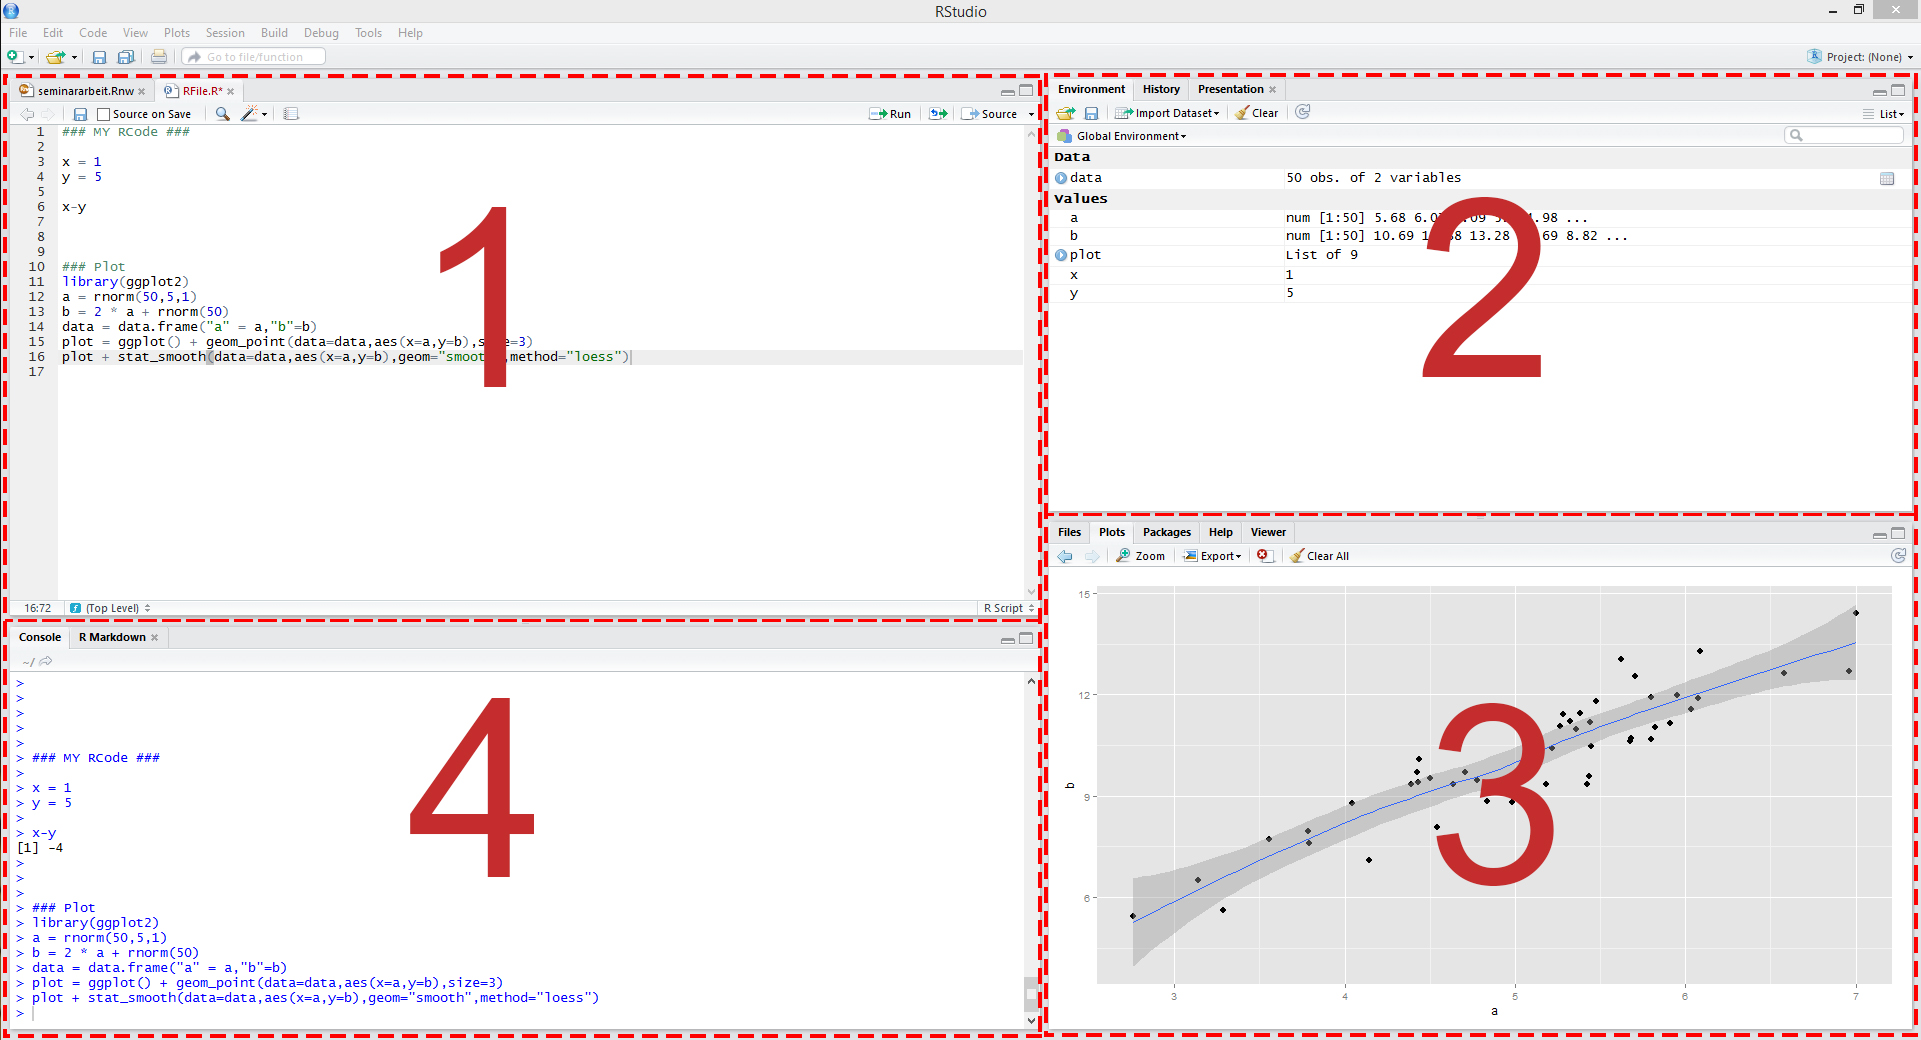
\includegraphics[width=1\linewidth]{images/rstudio} 

}

\caption{*RStudio*: the four panes}\label{fig:unnamed-chunk-7}
\end{figure}

\subsubsection*{\texorpdfstring{\texttt{R}
Basics}{ Basics}}\label{basics}
\addcontentsline{toc}{subsubsection}{\texttt{R} Basics}

This section is meant for those who have never worked with \texttt{R} or
\emph{RStudio}. If you at least know how to create objects and call
functions, you can skip it. If you would like to refresh your memories
or get a feeling for how to work with \emph{RStudio}, keep reading.

First of all start \emph{RStudio} and create a new R Script by selecting
\emph{File}, \emph{New File}, \emph{R Script}. In the editor pane type

\begin{Shaded}
\begin{Highlighting}[]
\DecValTok{1} \OperatorTok{+}\StringTok{ }\DecValTok{1}
\end{Highlighting}
\end{Shaded}

and click on the button labeled \emph{Run} in the top right corner of
the editor. By doing so, your line of code is send to the console and
the result of this operation should be displayed right underneath it. As
you can see, \texttt{R} works just like a calculator. You can do all the
arithmetic calculations by using the corresponding operator (+, - , *, /
or \^{}). If you are not sure what the last operator does, try it out
and check the results.

\subsubsection*{Vectors}\label{vectors}
\addcontentsline{toc}{subsubsection}{Vectors}

\texttt{R} is of course more sophisticated than that. We can work with
variables or more generally objects. Objects are defined by using the
assignment operator \texttt{<-}. To create a variable named \texttt{x}
which contains the value \texttt{10} type \texttt{x\ \textless{}-\ 10}
and click the button \emph{Run} yet again. The new variable should have
appeared in the environment pane on the top right. The console however
did not show any results, because our line of code did not contain any
call that creates output. When you now type \texttt{x} in the console
and hit return, you ask \texttt{R} to show you the value of \texttt{x}
and the corresponding value should be printed in the console.

\texttt{x} is a scalar, a vector of length \(1\). You can easily create
longer vectors by using the function \texttt{c()} (\emph{c} for
``concatenate'' or ``combine''). To create a vector \texttt{y}
containing the numbers \(1\) to \(5\) and print it, do the following.

\begin{Shaded}
\begin{Highlighting}[]
\NormalTok{y <-}\StringTok{ }\KeywordTok{c}\NormalTok{(}\DecValTok{1}\NormalTok{, }\DecValTok{2}\NormalTok{, }\DecValTok{3}\NormalTok{, }\DecValTok{4}\NormalTok{, }\DecValTok{5}\NormalTok{)}
\NormalTok{y}
\end{Highlighting}
\end{Shaded}

\begin{verbatim}
## [1] 1 2 3 4 5
\end{verbatim}

You can also create a vector of letters or words. For now just remember
that characters have to be surrounded by quotes, else wise they will be
parsed as object names.

\begin{Shaded}
\begin{Highlighting}[]
\NormalTok{hello <-}\StringTok{ }\KeywordTok{c}\NormalTok{(}\StringTok{"Hello"}\NormalTok{, }\StringTok{"World"}\NormalTok{)}
\end{Highlighting}
\end{Shaded}

Here we have created a vector of length 2 containing the words
\texttt{Hello} and \texttt{World}.

Do not forget to save your script! To do so, select \emph{File},
\emph{Save}.

\subsubsection*{Functions}\label{functions}
\addcontentsline{toc}{subsubsection}{Functions}

You have seen the function \texttt{c()} that can be used to combine
objects. In general, function calls look all the same, a function name
is always followed by round parentheses. Sometimes, the parentheses
include arguments

Here are two simple examples.

\begin{Shaded}
\begin{Highlighting}[]
\NormalTok{z <-}\StringTok{ }\KeywordTok{seq}\NormalTok{(}\DataTypeTok{from =} \DecValTok{1}\NormalTok{, }\DataTypeTok{to =} \DecValTok{5}\NormalTok{, }\DataTypeTok{by =} \DecValTok{1}\NormalTok{)}

\KeywordTok{mean}\NormalTok{(}\DataTypeTok{x =}\NormalTok{ z)}
\end{Highlighting}
\end{Shaded}

\begin{verbatim}
## [1] 3
\end{verbatim}

In the first line we use a function called \texttt{seq} to create the
exact same vector as we did in the previous section but naming it
\texttt{z}. The function takes on the arguments \texttt{from},
\texttt{to} and \texttt{by} which should be self-explaining. The
function \texttt{mean()} computes the arithmetic mean of its argument
\texttt{x}. Since we pass the vector \texttt{z} as the argument
\texttt{x} to \texttt{mean()}, the result is \texttt{3}!

If you are not sure what argument a function expects you may consult the
function's documentation. Let's say we are not sure how the arguments
required for \texttt{seq()} work. Then we can type \texttt{?seq} in the
console and by hitting return the documentation page for that function
pops up in the lower right pane of \emph{RStudio}. In there, the section
\emph{Arguments} holds the information we seek.

On the bottom of almost every help page you find examples on how to use
the corresponding functions. This is very helpful for beginners and we
recommend to look out for those.

\chapter{Introduction to Time Series Regression and
Forecasting}\label{introduction-to-time-series-regression-and-forecasting}

Time series data is data that is collected for a single entitity over
time. This is fundamentally different from cross-section data which is
data on multiple entities at the same point in time. Time series data
allows estimation of the effect on \(Y\) of a change in \(X\) \emph{over
time}. This is what econometricians call a \emph{dynamic causal effect}.
Let us go back to the application to cigarette consumption of Chapter 12
where we were interested in estimating the effect on cigarette demand of
a price increase caused by a raise of the general sales tax. One might
use time series data to assess the causal effect of a tax increase on
smoking both initially and in subsequent periods.

Another application of time series data is forecasting. For example,
weather services use time series models to predict tomorrow's average
temperatur using todays average termperature and average termperatures
of the past. To motivate an economic example, central banks are
interested in forecasting next month's unemployment rates.

The remainder of the book deals with the econometric techniques for the
analysis of time series data and application of the latter to problems
of forecasting and estimation of dynamic causal effects. This section
covers the basic concepts presented in Chapter 14 of the book, explains
how to visualize time series data and demonstrates how to estimate
simple autoregressive models, where the regressors are past values of
the dependent variable or other variables. In this context we will also
discuss the concept of stationarity, an important property which has
far-reaching consequences since it determines whether the past of a
series has any power in explaining the series' future.

Most empirical applications in this chapter are concerned with
forecasting and use data on U.S. macroeconomic indicators or financial
time series like Gross Domestic Product (GDP), the unemployment rate or
excess stock returns.

The following packages and their dependencies are needed for
reproduction of the code chunks presented throughout this chapter:

\begin{itemize}
\tightlist
\item
  \texttt{AER}
\item
  \texttt{dynlm}
\item
  \texttt{forecast}
\item
  \texttt{readxl}
\item
  \texttt{stargazer}
\item
  \texttt{scales}
\item
  \texttt{quantmod}
\end{itemize}

\section{Using Regression Models for
Forecasting}\label{using-regression-models-for-forecasting}

What is the difference between estimating models for assessment of
causal effects and forecasting? Consider again the simple example of
estimating the casual effect of the student-teacher ratio on test scores
introduced in Chapter 4.

\begin{Shaded}
\begin{Highlighting}[]
\KeywordTok{library}\NormalTok{(AER)}
\KeywordTok{data}\NormalTok{(CASchools)   }
\NormalTok{CASchools}\OperatorTok{$}\NormalTok{STR <-}\StringTok{ }\NormalTok{CASchools}\OperatorTok{$}\NormalTok{students}\OperatorTok{/}\NormalTok{CASchools}\OperatorTok{$}\NormalTok{teachers       }
\NormalTok{CASchools}\OperatorTok{$}\NormalTok{score <-}\StringTok{ }\NormalTok{(CASchools}\OperatorTok{$}\NormalTok{read }\OperatorTok{+}\StringTok{ }\NormalTok{CASchools}\OperatorTok{$}\NormalTok{math)}\OperatorTok{/}\DecValTok{2}

\NormalTok{mod <-}\StringTok{ }\KeywordTok{lm}\NormalTok{(score }\OperatorTok{~}\StringTok{ }\NormalTok{STR, }\DataTypeTok{data =}\NormalTok{ CASchools)}
\NormalTok{mod}
\end{Highlighting}
\end{Shaded}

\begin{verbatim}
## 
## Call:
## lm(formula = score ~ STR, data = CASchools)
## 
## Coefficients:
## (Intercept)          STR  
##      698.93        -2.28
\end{verbatim}

As has been stressed in Chapter 6, the estimate of the coefficient on
the student-teacher ratio does not have causal interpretation due to
omitted variable bias. However, in terms deciding which school to send
her child to, it might nevertheless be appealig for a parent to use
\texttt{mod} for forecasting test scores in schooling districts where no
public data about on scores are available.

As an example, assume that the average class in a district has \(25\)
students. There is no such thing as a perfect forecast but the following
one-liner might be helpful for the parent to decide.

\begin{Shaded}
\begin{Highlighting}[]
\KeywordTok{predict}\NormalTok{(mod, }\DataTypeTok{newdata =} \KeywordTok{data.frame}\NormalTok{(}\StringTok{"STR"}\NormalTok{ =}\StringTok{ }\DecValTok{25}\NormalTok{))}
\end{Highlighting}
\end{Shaded}

\begin{verbatim}
##        1 
## 641.9377
\end{verbatim}

In a time series context, the parent could use data on present and past
years test scores to forecast next years test scores --- a typical
application for an autoregressive model.

\section{Time Series Data and Serial
Correlation}\label{time-series-data-and-serial-correlation}

GDP measures the productivity of an economy. It is commonly defined as
the value of goods and services produced over a given time period. The
data set us\_macro\_quarterly.xlsx is provided by the authors and can be
downloaded
\href{http://wps.aw.com/aw_stock_ie_3/178/45691/11696965.cw/index.html}{here}.
It provides quarterly data on U.S. real (i.e.~inflation adjusted) GDP
from years 1947 to 2004.

As before, a good point to start with in pre-estimation is plotting the
data. The package \texttt{quantmod} provides some very convenient
functions for plotting and computing with time series data. We also load
the package \texttt{readxl} to read the data into R.

\begin{Shaded}
\begin{Highlighting}[]
\CommentTok{# attach the package `quantmod`}
\KeywordTok{library}\NormalTok{(quantmod)}
\end{Highlighting}
\end{Shaded}

We begin by importing the data set.

\begin{Shaded}
\begin{Highlighting}[]
\CommentTok{# load US macroeconomic data}
\NormalTok{USMacroSWQ <-}\StringTok{ }\KeywordTok{read_xlsx}\NormalTok{(}\StringTok{"Data/us_macro_quarterly.xlsx"}\NormalTok{,}
                         \DataTypeTok{sheet =} \DecValTok{1}\NormalTok{,}
                         \DataTypeTok{col_types =} \KeywordTok{c}\NormalTok{(}\StringTok{"text"}\NormalTok{, }\KeywordTok{rep}\NormalTok{(}\StringTok{"numeric"}\NormalTok{, }\DecValTok{9}\NormalTok{))}
\NormalTok{                        )}

\CommentTok{# format date column}
\NormalTok{USMacroSWQ}\OperatorTok{$}\NormalTok{X__}\DecValTok{1}\NormalTok{ <-}\StringTok{ }\KeywordTok{as.yearqtr}\NormalTok{(USMacroSWQ}\OperatorTok{$}\NormalTok{X__}\DecValTok{1}\NormalTok{, }\DataTypeTok{format =} \StringTok{"%Y:0%q"}\NormalTok{)}

\CommentTok{# adjust column names}
\KeywordTok{colnames}\NormalTok{(USMacroSWQ) <-}\StringTok{ }\KeywordTok{c}\NormalTok{(}\StringTok{"Date"}\NormalTok{, }\StringTok{"GDPC96"}\NormalTok{, }\StringTok{"JAPAN_IP"}\NormalTok{, }\StringTok{"PCECTPI"}\NormalTok{, }
                          \StringTok{"GS10"}\NormalTok{, }\StringTok{"GS1"}\NormalTok{, }\StringTok{"TB3MS"}\NormalTok{, }\StringTok{"UNRATE"}\NormalTok{, }\StringTok{"EXUSUK"}\NormalTok{, }\StringTok{"CPIAUCSL"}\NormalTok{)}
\end{Highlighting}
\end{Shaded}

When dealing with time series data in R it is preferable to work with
time-series objects that keep track of the frequency of the data and are
extensible. In what follows we will use objects of the class xts, see
\texttt{?xts}. Since the data in \texttt{USMacroSWQ} are in quarterly
frequence we convert the first column to \texttt{yearqtr} format before
generating the xts object \texttt{GDP}.

The function \texttt{Delt()} from the package \texttt{quantmod} computes
growth rates. We anualize the quarterly changes to obtain anual growth
rates as \[Rate_{annual} = (1+Rate_{quarterly})^4-1.\]

\begin{Shaded}
\begin{Highlighting}[]
\CommentTok{# GDP series as xts object}
\NormalTok{GDP <-}\StringTok{ }\KeywordTok{xts}\NormalTok{(USMacroSWQ}\OperatorTok{$}\NormalTok{GDPC96, USMacroSWQ}\OperatorTok{$}\NormalTok{Date)[}\StringTok{"1960::2013"}\NormalTok{]}

\CommentTok{# GDP growth series as xts object}
\NormalTok{GDPGrowth <-}\StringTok{ }\KeywordTok{xts}\NormalTok{(}\DecValTok{400} \OperatorTok{*}\StringTok{ }\KeywordTok{log}\NormalTok{(GDP}\OperatorTok{/}\KeywordTok{lag}\NormalTok{(GDP)))}
\end{Highlighting}
\end{Shaded}

The following code chunks reproduce Figure 14.1 of the book.

\begin{Shaded}
\begin{Highlighting}[]
\CommentTok{# reproduce figure 14.1 (a) of the book}
\KeywordTok{plot}\NormalTok{(}\KeywordTok{log}\NormalTok{(}\KeywordTok{as.zoo}\NormalTok{(GDP)),}
     \DataTypeTok{col =} \StringTok{"steelblue"}\NormalTok{,}
     \DataTypeTok{lwd =} \DecValTok{2}\NormalTok{,}
     \DataTypeTok{ylab =} \StringTok{"Logarithm"}\NormalTok{,}
     \DataTypeTok{xlab =} \StringTok{"Date"}\NormalTok{,}
     \DataTypeTok{main =} \StringTok{"U.S. Quarterly Real GDP"}
\NormalTok{     )}
\end{Highlighting}
\end{Shaded}

\begin{center}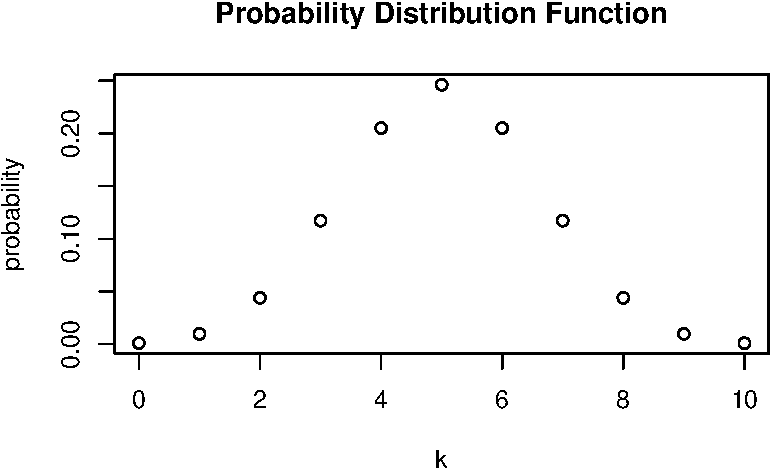
\includegraphics{URFITE_files/figure-latex/unnamed-chunk-19-1} \end{center}

\begin{Shaded}
\begin{Highlighting}[]
\CommentTok{# reproduce figure 14.1 (b) of the book}
\KeywordTok{plot}\NormalTok{(}\KeywordTok{as.zoo}\NormalTok{(GDPGrowth),}
     \DataTypeTok{col =} \StringTok{"steelblue"}\NormalTok{,}
     \DataTypeTok{lwd =} \DecValTok{2}\NormalTok{,}
     \DataTypeTok{ylab =} \StringTok{"Logarithm"}\NormalTok{,}
     \DataTypeTok{xlab =} \StringTok{"Date"}\NormalTok{,}
     \DataTypeTok{main =} \StringTok{"Growth Rates in U.S. Real GDP"}
\NormalTok{     )}
\end{Highlighting}
\end{Shaded}

\begin{center}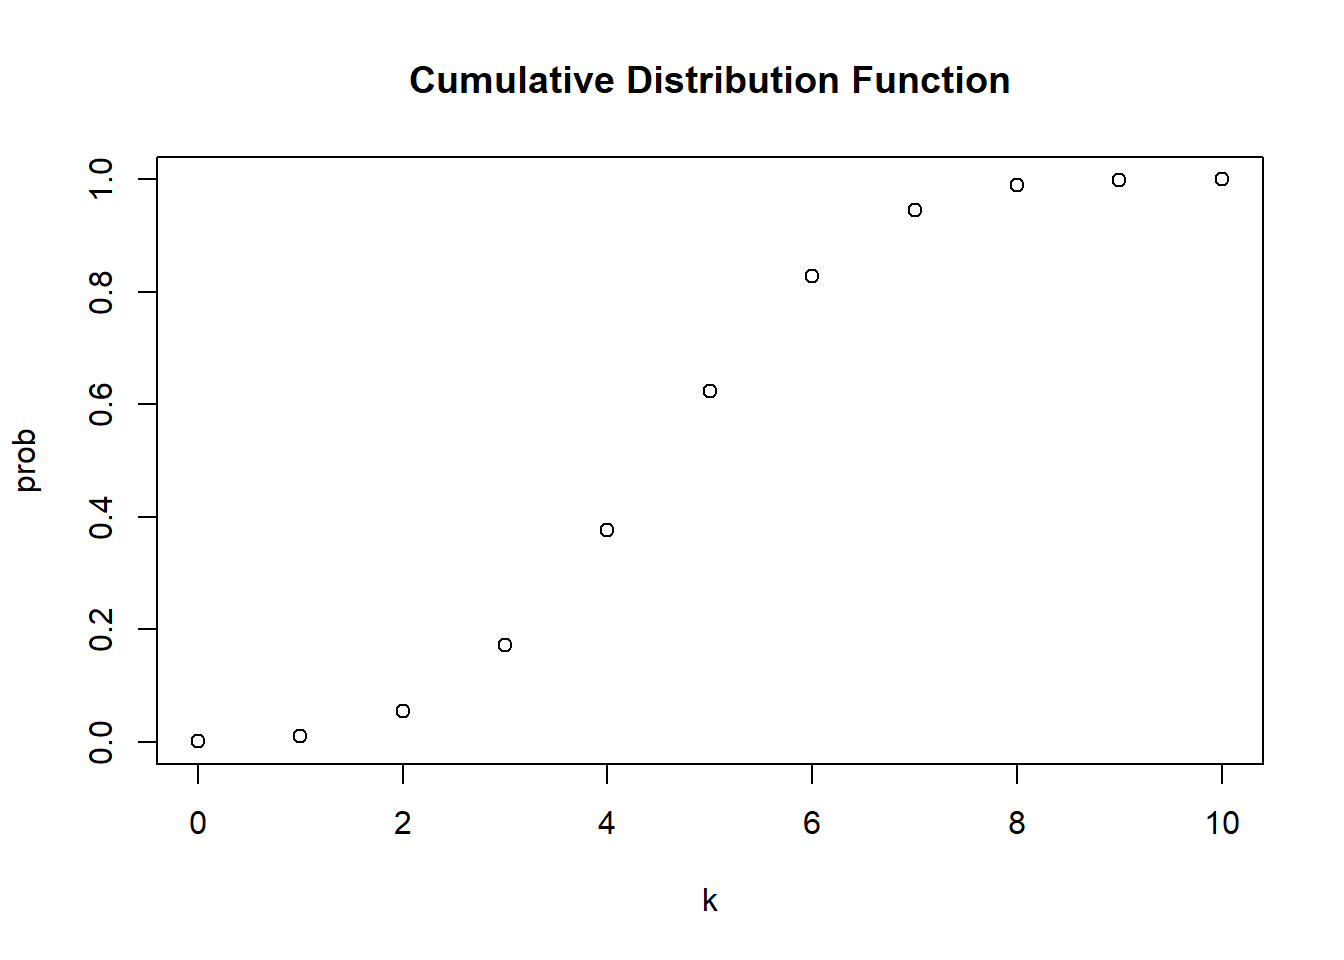
\includegraphics{URFITE_files/figure-latex/unnamed-chunk-20-1} \end{center}

\subsection*{Notation, Lags, Differences, Logarithms and Growth
Rates}\label{notation-lags-differences-logarithms-and-growth-rates}
\addcontentsline{toc}{subsection}{Notation, Lags, Differences,
Logarithms and Growth Rates}

If observations of a variable \(Y\) are recorded over time, we denote
\(Y_t\) the value observed at time \(t\). The period between two
sequential observations \(Y_t\) and \(Y_{t-1}\) is a unit of time:
hours, days, weeks, months, quarters, years and so on. Key Concept 14.1
introduces the essential terminology and notation for time series data
we will use in the subsequent sections.

Key Concept 14.1

Lags, First Differences, Logarithms and Growth Rates

\begin{itemize}
\item
  Previous values of a time series are called \emph{lags}. The first lag
  of \(Y_t\) is \(Y_{t-1}\). The \(j^{th}\) lag of \(Y_t\) is
  \(Y_{t-j}\). In R, lags of univariate or multivariate time series are
  conveniently computed by \texttt{lag()}, see \texttt{?lag}
\item
  Sometimes we need to work with a differenced series. The first
  difference of a series is \(\Delta Y_{t} = Y_t - Y_{t-1}\), the
  difference between periods \(t\) and \(t-1\). If \texttt{Y} is a time
  series, the series of first differences is computed as
  \texttt{Y-lag(Y)}.
\item
  It may be convenient to work with the first difference in logarithms
  of a series. We denote this by
  \(\Delta \log(Y_t) = \log(Y_t) - \log(Y_{t-1})\). For a time series
  \texttt{Y}, this is obtained using \texttt{log(Y/lag(Y))}.
\item
  \(100 \Delta \log (Y_t)\) is an approximation for the percentage
  change between \(Y_t\) and \(Y_{t-1}\).
\end{itemize}

The definitions made in Key Concept 14.1 are useful because of two
properties that are common to many economic time series:

\begin{itemize}
\item
  Exponential growth: some economic series grow approximately
  exponentially such that taking the logarithm of these series makes
  them approximately linear.
\item
  The standard deviation of many economic time series is approximately
  proportional to their level. Therefore, the standard deviation of the
  logarithm of such a series is approximately constant.
\end{itemize}

Furthermore, it is common to report rates of growth in macroeconomic
series which is why \(\log\)-differences are often used.

Table 14.1 of the book presents the quaterly U.S. GDP time series, its
logarithm, the anualized growth rate and the first lag of the anualized
growth rate series for the period 2012:Q1 - 2013:Q1. The following
simple function can be used to compute these quantities for a quaterly
time series \texttt{series}.

\begin{Shaded}
\begin{Highlighting}[]
\CommentTok{# compute logarithms, annual growth rates and 1st lag of growth rates}
\NormalTok{quants <-}\StringTok{ }\ControlFlowTok{function}\NormalTok{(series) \{}
\NormalTok{  s <-}\StringTok{ }\NormalTok{series}
  \KeywordTok{return}\NormalTok{(}
    \KeywordTok{data.frame}\NormalTok{(}\StringTok{"Lead"}\NormalTok{ =}\StringTok{ }\NormalTok{s,}
               \StringTok{"Logarithm"}\NormalTok{ =}\StringTok{ }\KeywordTok{log}\NormalTok{(s),}
               \StringTok{"AnnualGrowthRate"}\NormalTok{ =}\StringTok{ }\DecValTok{400} \OperatorTok{*}\StringTok{ }\KeywordTok{log}\NormalTok{(s}\OperatorTok{/}\KeywordTok{lag}\NormalTok{(s)),}
               \StringTok{"1stLagAnnualGrowthRate"}\NormalTok{ =}\StringTok{ }\KeywordTok{lag}\NormalTok{(}\DecValTok{400} \OperatorTok{*}\StringTok{ }\KeywordTok{log}\NormalTok{(s}\OperatorTok{/}\KeywordTok{lag}\NormalTok{(s)))}
\NormalTok{      )}
\NormalTok{  )}
\NormalTok{\}}
\end{Highlighting}
\end{Shaded}

Notice that the annual growth rate is computed using the approximation
\[ Annual Growth Y_t = 400 \cdot \left[\log(Y_t) - \log(Y_{t-1})\right] \]
discussed in Key Concept 14.1.

We call \texttt{quants()} on observations for the period 2011 Q3 - 2013
Q1.

\begin{Shaded}
\begin{Highlighting}[]
\KeywordTok{quants}\NormalTok{(GDP[}\StringTok{"2011-07::2013-01"}\NormalTok{])}
\end{Highlighting}
\end{Shaded}

\begin{verbatim}
##             Lead Logarithm AnnualGrowthRate X1stLagAnnualGrowthRate
## 2011 Q3 15062.14  9.619940               NA                      NA
## 2011 Q4 15242.14  9.631819        4.7518062                      NA
## 2012 Q1 15381.56  9.640925        3.6422231               4.7518062
## 2012 Q2 15427.67  9.643918        1.1972004               3.6422231
## 2012 Q3 15533.99  9.650785        2.7470216               1.1972004
## 2012 Q4 15539.63  9.651149        0.1452808               2.7470216
## 2013 Q1 15583.95  9.653997        1.1392015               0.1452808
\end{verbatim}

\subsubsection*{Autocorrelation}\label{autocorrelation}
\addcontentsline{toc}{subsubsection}{Autocorrelation}

Observations of a time series are typically correlated. This type of
correlation is called \emph{autocorrelation} or \emph{serial
correlation}. Key Concept 14.2 summarizes the concepts of population
autocovariance and population autocorrelation and shows how to compute
their sample equivalents.

Key Concept 14.2

Autocorrelation and Autocovariance

The covariance between \(Y_t\) and its \(j^{th}\) lag, \(Y_{t-j}\), is
called the \(j^{th}\) \emph{autocovariance} of the series \(Y_t\). The
\(j^{th}\) \emph{autocorrelation coefficient}, also called the
\emph{serial correlation coefficient}, measures the correlation between
\(Y_t\) and \(Y_{t-j}\).

We thus have

\begin{align*}
  j^{th} \text{autocovariance} =& \, Cov(Y_t,Y_{t-j}), \\
  j^{th} \text{autocorrelation} = \rho_j =& \, \rho_{Y_t,Y_{t-j}} = \frac{Cov(Y_t,Y_{t-j)}}{\sqrt{Var(Y_t)Var{Y_{t-j}}}}.
\end{align*}

Population Autocovariance and population autocorrelation can be
estimated by \(\widehat{Cov(Y_t,Y_{t-j})}\), the sample autocovariance,
and \(\widehat{\rho}_j\), the sample autocorrelation.

\begin{align*}
  \widehat{Cov(Y_t,Y_{t-j})} =& \, \frac{1}{T} \sum_{t=j+1}^T (Y_t - \overline{Y}_{j+1:T})(Y_{t-j} - \overline{Y}_{1:T-j}) \\
  \widehat{\rho}_j =& \, \frac{\widehat{Cov(Y_t,Y_{t-j})}}{\widehat{Var(Y_t)}}.
\end{align*}

In R the function \texttt{acf()} from the package stats computes the
sample autocovariance or the sample autocorrelation function.

Using \texttt{acf()} it is straightforward to compute the first four
sample autocorrelations of the series \texttt{GDPGrowth}.

\begin{Shaded}
\begin{Highlighting}[]
\KeywordTok{acf}\NormalTok{(}\KeywordTok{na.omit}\NormalTok{(GDPGrowth), }\DataTypeTok{lag.max =} \DecValTok{4}\NormalTok{, }\DataTypeTok{plot =}\NormalTok{ F)}
\end{Highlighting}
\end{Shaded}

\begin{verbatim}
## 
## Autocorrelations of series 'na.omit(GDPGrowth)', by lag
## 
##  0.00  0.25  0.50  0.75  1.00 
## 1.000 0.352 0.273 0.114 0.106
\end{verbatim}

This is evidence that there is mild positive autocorrelation in the
growth of GDP: if GDP grows faster than average in one period, there is
a tendency that it grows faster than average in the following periods.

\subsubsection*{Other Examples of Economic Time
Series}\label{other-examples-of-economic-time-series}
\addcontentsline{toc}{subsubsection}{Other Examples of Economic Time
Series}

Figure 14.2 of the book presents four plots. The U.S. unemployment rate,
the U.S. Dollar / British Pound exchange rate, The logarithm of the
Janapese industrial production index as well as daily changes in the
Whilshire 5000 stock price index, a financial time series. The next code
chunk reproduces the plots of the three macroenomic series and adds
percentage changes in the daily values of the New York Stock Exchange
Composite index as a fourth one (the data set \texttt{NYSESW} comes with
the \texttt{AER} package).

\begin{Shaded}
\begin{Highlighting}[]
\CommentTok{# define series as xts objects}
\NormalTok{USUnemp <-}\StringTok{ }\KeywordTok{xts}\NormalTok{(USMacroSWQ}\OperatorTok{$}\NormalTok{UNRATE, USMacroSWQ}\OperatorTok{$}\NormalTok{Date)[}\StringTok{"1960::2013"}\NormalTok{]}

\NormalTok{DollarPoundFX <-}\StringTok{ }\KeywordTok{xts}\NormalTok{(USMacroSWQ}\OperatorTok{$}\NormalTok{EXUSUK, USMacroSWQ}\OperatorTok{$}\NormalTok{Date)[}\StringTok{"1960::2013"}\NormalTok{]}
  
\NormalTok{JPIndProd <-}\StringTok{ }\KeywordTok{xts}\NormalTok{(}\KeywordTok{log}\NormalTok{(USMacroSWQ}\OperatorTok{$}\NormalTok{JAPAN_IP), USMacroSWQ}\OperatorTok{$}\NormalTok{Date)[}\StringTok{"1960::2013"}\NormalTok{]}

\KeywordTok{data}\NormalTok{(}\StringTok{"NYSESW"}\NormalTok{)  }
\NormalTok{NYSESW <-}\StringTok{ }\KeywordTok{xts}\NormalTok{(}\KeywordTok{Delt}\NormalTok{(NYSESW))}
\end{Highlighting}
\end{Shaded}

\begin{Shaded}
\begin{Highlighting}[]
\KeywordTok{par}\NormalTok{(}\DataTypeTok{mfrow =} \KeywordTok{c}\NormalTok{(}\DecValTok{2}\NormalTok{, }\DecValTok{2}\NormalTok{))}

\KeywordTok{plot}\NormalTok{(}\KeywordTok{as.zoo}\NormalTok{(USUnemp),}
     \DataTypeTok{col =} \StringTok{"steelblue"}\NormalTok{,}
     \DataTypeTok{lwd =} \DecValTok{2}\NormalTok{,}
     \DataTypeTok{ylab =} \StringTok{"Percent"}\NormalTok{,}
     \DataTypeTok{xlab =} \StringTok{"Date"}\NormalTok{,}
     \DataTypeTok{main =} \StringTok{"US Unemployment Rate"}\NormalTok{,}
     \DataTypeTok{cex.main =} \DecValTok{1}
\NormalTok{)}

\KeywordTok{plot}\NormalTok{(}\KeywordTok{as.zoo}\NormalTok{(DollarPoundFX),}
     \DataTypeTok{col =} \StringTok{"steelblue"}\NormalTok{,}
     \DataTypeTok{lwd =} \DecValTok{2}\NormalTok{,}
     \DataTypeTok{ylab =} \StringTok{"Dollar per pound"}\NormalTok{,}
     \DataTypeTok{xlab =} \StringTok{"Date"}\NormalTok{,}
     \DataTypeTok{main =} \StringTok{"U.S. Dollar / B. Pound Exchange Rate"}\NormalTok{,}
     \DataTypeTok{cex.main =} \DecValTok{1}
\NormalTok{)}

\KeywordTok{plot}\NormalTok{(}\KeywordTok{as.zoo}\NormalTok{(JPIndProd),}
     \DataTypeTok{col =} \StringTok{"steelblue"}\NormalTok{,}
     \DataTypeTok{lwd =} \DecValTok{2}\NormalTok{,}
     \DataTypeTok{ylab =} \StringTok{"Logarithm"}\NormalTok{,}
     \DataTypeTok{xlab =} \StringTok{"Date"}\NormalTok{,}
     \DataTypeTok{main =} \StringTok{"Japanese Industrial Production"}\NormalTok{,}
     \DataTypeTok{cex.main =} \DecValTok{1}
\NormalTok{)}

\KeywordTok{plot}\NormalTok{(}\KeywordTok{as.zoo}\NormalTok{(NYSESW),}
     \DataTypeTok{col =} \StringTok{"steelblue"}\NormalTok{,}
     \DataTypeTok{lwd =} \DecValTok{2}\NormalTok{,}
     \DataTypeTok{ylab =} \StringTok{"Percent per Day"}\NormalTok{,}
     \DataTypeTok{xlab =} \StringTok{"Date"}\NormalTok{,}
     \DataTypeTok{main =} \StringTok{"New York Stock Exchange Composite Index"}\NormalTok{,}
     \DataTypeTok{cex.main =} \DecValTok{1}
\NormalTok{)}
\end{Highlighting}
\end{Shaded}

\begin{center}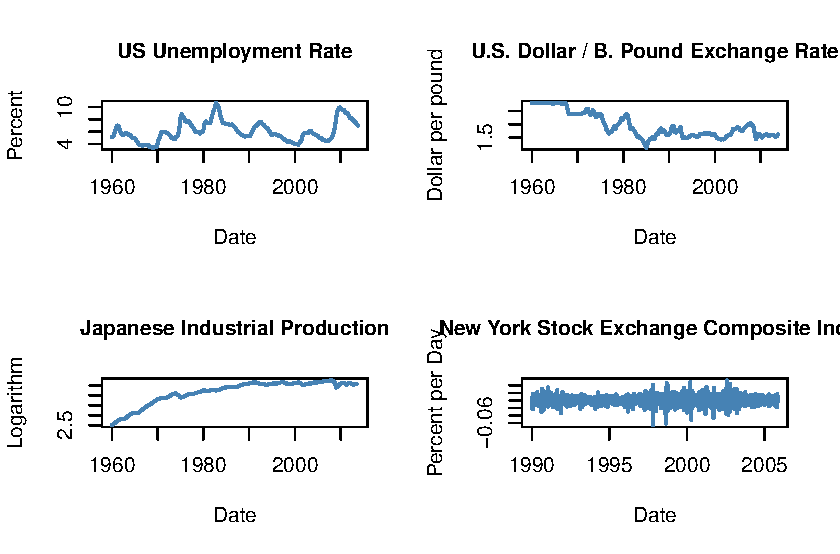
\includegraphics{URFITE_files/figure-latex/unnamed-chunk-25-1} \end{center}

Note that the series show quite different characteristics. The
unemployment rate increases during recessions and declines in times of
economic recoveries and growth. The Dollar/Pund exchange rates shows a
deterministic patern until the end of the Bretton Woods system. Japans
industrial production exhibits an upward trend and decreasing growth.
Daily changes in the New York Stock Exchange composite index seem to be
random around the zero line. The sample autocorrelations confirm this
conjecture.

\begin{Shaded}
\begin{Highlighting}[]
\CommentTok{# compute sample autocorrelation for the NYSESW series}
\KeywordTok{acf}\NormalTok{(}\KeywordTok{na.omit}\NormalTok{(NYSESW), }\DataTypeTok{plot =}\NormalTok{ F, }\DataTypeTok{lag.max =} \DecValTok{10}\NormalTok{)}
\end{Highlighting}
\end{Shaded}

\begin{verbatim}
## 
## Autocorrelations of series 'na.omit(NYSESW)', by lag
## 
##      0      1      2      3      4      5      6      7      8      9 
##  1.000  0.040 -0.016 -0.023  0.000 -0.036 -0.027 -0.059  0.013  0.017 
##     10 
##  0.004
\end{verbatim}

The first 10 sample autocorrelation coefficients are very close to zero.
Further evidence can be found by looking at the plot generated by
\texttt{acf()} by default.

\begin{Shaded}
\begin{Highlighting}[]
\KeywordTok{acf}\NormalTok{(}\KeywordTok{na.omit}\NormalTok{(NYSESW), }\DataTypeTok{main =} \StringTok{"Sample Autocorrelation for NYSESW Data"}\NormalTok{)}
\end{Highlighting}
\end{Shaded}

\begin{center}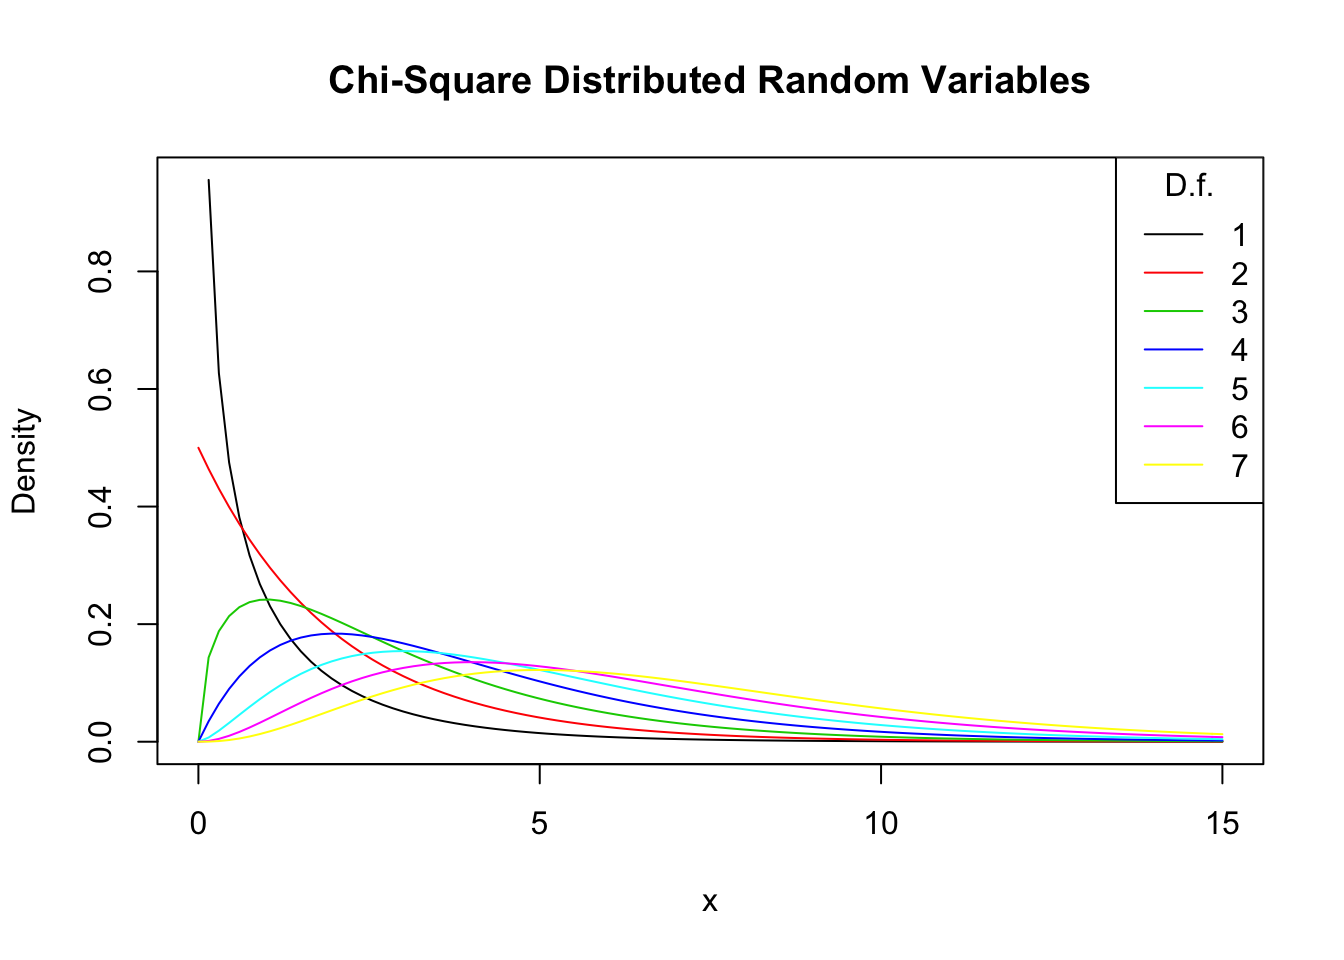
\includegraphics{URFITE_files/figure-latex/unnamed-chunk-27-1} \end{center}

The blue dashed lines represent an approximate \(95\%\) confidence
interval if there was no serial correlation. If a sample autocorrelation
lies beyond these bands, it is statistically different from zero. For
most lags we see that the sample autocorrelation does not exceed the
confidence bands and there are only a few cases that lie marginally
beyond the limits.

Furthermore, note that NYSWSW series shows a pattern which
econometricians call \emph{volatility clustering}: there are periods of
high and periods of low variance. This is common for many financial time
series.

\section{Autoregressions}\label{autoregressions}

Growth forecasts are important for many economic entitites. For example,
the production setor relies on forecasts of GDP growth published by the
central bank when deciding on future budgets and production plans.
Autoregressive models are heavily used in economic forecasting. An
autoregressive model relates a time series variable to its past values.
This chapter discusses the basic ideas of autoregressions models, shows
how they are estimated and discusses an application to forecasting of
GDP growth using R.

\subsubsection*{The First-Order Autoregressive
Model}\label{the-first-order-autoregressive-model}
\addcontentsline{toc}{subsubsection}{The First-Order Autoregressive
Model}

It is intuitive that the immediate past of a time series should have
power to predict its near future. The simplest autoregressive model uses
only the most recent outcome of the time series observed to predict
future values. Such a model is called a first-order autoregressive model
which is often abbriviated AR(1), where the 1 indicates that the order
of autoregression is one.

\begin{align*}
  Y_t = \beta_0 + \beta_1 Y_{t-1} + u_t
\end{align*}

is the AR(1) population model of a time series \(Y_t\).

For the GDP growth series, an autoregressive model of order one uses
only the information on GDP growth observed in the last quarter to
predict a future growth rate. The first-order autoregression model of
the GDP growth rate can be estimated by computing OLS estimates in the
regression of \(GDPGR_t\) on \(GDPGR_{t-1}\),

\begin{align}
  \widehat{GDPGR}_t = \beta_0 + \beta_1 GDPGR_{t-1} + u_t. \label{eq:GDPGRAR1}
\end{align}

Following the book we use data from 1962 to 2012 to estimate
\eqref{eq:GDPGRAR1}. This is easily done with the function
\texttt{ar.ols()} from package stats.

\begin{Shaded}
\begin{Highlighting}[]
\CommentTok{# subset data}
\NormalTok{GDPGRSub <-}\StringTok{ }\NormalTok{GDPGrowth[}\StringTok{"1962::2012"}\NormalTok{]}

\CommentTok{# estimate the model}
\KeywordTok{ar.ols}\NormalTok{(GDPGRSub, }
       \DataTypeTok{order.max =} \DecValTok{1}\NormalTok{, }
       \DataTypeTok{demean =}\NormalTok{ F, }
       \DataTypeTok{intercept =}\NormalTok{ T)}
\end{Highlighting}
\end{Shaded}

\begin{verbatim}
## 
## Call:
## ar.ols(x = GDPGRSub, order.max = 1, demean = F, intercept = T)
## 
## Coefficients:
##      1  
## 0.3384  
## 
## Intercept: 1.995 (0.2993) 
## 
## Order selected 1  sigma^2 estimated as  9.886
\end{verbatim}

We can check that the computations done by \texttt{ar.ols()} are the
same as done by \texttt{lm()}.

\begin{Shaded}
\begin{Highlighting}[]
\CommentTok{# length of data set}
\NormalTok{N <-}\KeywordTok{length}\NormalTok{(GDPGRSub)}

\NormalTok{GDPGR_leads <-}\StringTok{ }\KeywordTok{as.numeric}\NormalTok{(GDPGRSub[}\OperatorTok{-}\DecValTok{1}\NormalTok{])}
\NormalTok{GDPGR_lags <-}\StringTok{ }\KeywordTok{as.numeric}\NormalTok{(GDPGRSub[}\OperatorTok{-}\NormalTok{N])}

\CommentTok{# estimate the model}
\NormalTok{armod <-}\StringTok{ }\KeywordTok{lm}\NormalTok{(GDPGR_leads }\OperatorTok{~}\StringTok{ }\NormalTok{GDPGR_lags)}
\NormalTok{armod}
\end{Highlighting}
\end{Shaded}

\begin{verbatim}
## 
## Call:
## lm(formula = GDPGR_leads ~ GDPGR_lags)
## 
## Coefficients:
## (Intercept)   GDPGR_lags  
##      1.9950       0.3384
\end{verbatim}

As usual, we may use \texttt{coeftest()} to obtain a robust summary on
the estimated regression coefficients.

\begin{Shaded}
\begin{Highlighting}[]
\CommentTok{# robust summary}
\KeywordTok{coeftest}\NormalTok{(armod, }\DataTypeTok{vcov. =} \KeywordTok{vcovHC}\NormalTok{(armod, }\DataTypeTok{type =} \StringTok{"HC1"}\NormalTok{))}
\end{Highlighting}
\end{Shaded}

\begin{verbatim}
## 
## t test of coefficients:
## 
##             Estimate Std. Error t value  Pr(>|t|)    
## (Intercept) 1.994986   0.351274  5.6793 4.691e-08 ***
## GDPGR_lags  0.338436   0.076188  4.4421 1.470e-05 ***
## ---
## Signif. codes:  0 '***' 0.001 '**' 0.01 '*' 0.05 '.' 0.1 ' ' 1
\end{verbatim}

Thus the estimated model is

\begin{align}
  \widehat{GDPGR}_t = \underset{(0.351)}{1.995} + \underset{(0.076)}{0.338} GDPGR_{t-1} \label{eq:gdpgrar1}.
\end{align}

Notice that we omit the first observation for \(GDPGR_{1962 \ Q1}\) from
the vector of the dependent variable since
\(GDPGR_{1962 \ Q1 - 1} = GDPGR_{1961 \ Q4}\), is not included in the
sample. Similarly, the last observation, \(GDPGR_{2012 \ Q4}\), is
excluded from the predictor vector since the data set does not include
\(GDPGR_{2012 \ Q4 + 1} = GDPGR_{2013 \ Q1}\). Put differently, when
estimating the model, one observation is lost because of the time series
structure of the data.

\subsubsection*{Forecasts and Forecast
Errors}\label{forecasts-and-forecast-errors}
\addcontentsline{toc}{subsubsection}{Forecasts and Forecast Errors}

Suppose a random variable \(Y_t\) follows an AR(1) model with an
intercept and that you have an OLS estimate of the model on the basis of
observations for \(T\) periods. Then you may use the AR(1) model to
obtain \(Y_{T+1\vert T}\), a forecast for \(Y_{T+1}\) using data up to
perdiod \(T\) where

\begin{align*}
  \widehat{Y}_{T+1\vert T} = \widehat{\beta}_0 + \widehat{\beta}_1 Y_T.
\end{align*}

The forecast error is

\begin{align*}
  \text{Forecast error} = Y_{T+1} - \widehat{Y}_{T+1\vert T}.
\end{align*}

\subsubsection*{Forecasts and Predicted
Values}\label{forecasts-and-predicted-values}
\addcontentsline{toc}{subsubsection}{Forecasts and Predicted Values}

Note that \emph{forecasted values} of \(Y_t\) are \emph{not} what we
refer to as \emph{OLS predicted values} of \(Y_t\). Also, the forecast
error is \emph{not} an OLS residual. Forecasts and forecast errors are
obtained using \emph{out-of-sample} values while predicted values and
residuals are computed for \emph{in-sample} values that were actually
observed and used in estimation of the model.

The root mean squared forecast error (RMSFE) measures the typical size
of the forecast error and is defined as

\begin{align*}
  RMSFE = \sqrt{E\left[\left(Y_{T+1} - \widehat{Y}_{T+1\vert T}\right)^2\right]}.
\end{align*}

\subsubsection*{Application to GDP
Growth}\label{application-to-gdp-growth}
\addcontentsline{toc}{subsubsection}{Application to GDP Growth}

Using \eqref{eq:gdpgrar1}, the estimated AR(1) model of GDP growth, we may
perform the forecast for GDP growth in 2013:Q1 (remember that the model
was estimated using data for periods 1962:Q1 - 2012:Q4 so 2013:Q1 is an
out of sample period). This is done by plugging
\(GDPGR_{2012:Q4} \approx 0.15\) in \eqref{eq:gdpgrar1},

\begin{align*}
  \widehat{GDPGR}_{2013:Q1} = 1.995 + 0.348 \cdot 0.15 = 2.047.
\end{align*}

The function \texttt{forecast()} from the forecast package has some
useful features for forecasting of time series data.

\begin{Shaded}
\begin{Highlighting}[]
\KeywordTok{library}\NormalTok{(forecast)}

\CommentTok{# assign GDP growth rate in 2012:Q4}
\NormalTok{new <-}\StringTok{ }\KeywordTok{data.frame}\NormalTok{(}\StringTok{"GDPGR_lags"}\NormalTok{ =}\StringTok{ }\NormalTok{GDPGR_leads[N}\OperatorTok{-}\DecValTok{1}\NormalTok{])}

\CommentTok{# forecast GDP growth rate in 2013:Q1}
\KeywordTok{forecast}\NormalTok{(armod, }\DataTypeTok{newdata =}\NormalTok{ new)}
\end{Highlighting}
\end{Shaded}

\begin{verbatim}
##   Point Forecast     Lo 80    Hi 80     Lo 95    Hi 95
## 1       2.044155 -2.036225 6.124534 -4.213414 8.301723
\end{verbatim}

Using \texttt{forecast()} we obtain the same point forecast of about
2.0, along with \(80\%\) and \(95\%\) forecast intervals. We conclude
that our AR(1) model forecasts GDP growth to be \(2\%\) in 2013:Q1.

How accurate is this forecast? First, notice that the forecast error is
pretty big: \(GDPGR_{2013:Q1} \approx 1.1\%\) while our forecast is
\(2\%\). Second, by calling \texttt{summary()} on \texttt{armod} we find
that the model explains only little of the variation in the growth rate
of GDP and the \(SER\) is about \(3.16\). Leaving aside forecast
uncertainty due to estimation of the model coefficients \(\beta_0\) and
\(\beta_1\), the \(RMSFE\) must be at least \(3.16\%\) which is pretty
inaccurate.

\begin{Shaded}
\begin{Highlighting}[]
\CommentTok{# compute the forecast error}
\KeywordTok{forecast}\NormalTok{(armod, }\DataTypeTok{newdata =}\NormalTok{ new)}\OperatorTok{$}\NormalTok{mean }\OperatorTok{-}\StringTok{ }\NormalTok{GDPGrowth[}\StringTok{"2013"}\NormalTok{][}\DecValTok{1}\NormalTok{]}
\end{Highlighting}
\end{Shaded}

\begin{verbatim}
##                 x
## 2013 Q1 0.9049532
\end{verbatim}

\begin{Shaded}
\begin{Highlighting}[]
\CommentTok{# R^2}
\KeywordTok{summary}\NormalTok{(armod)}\OperatorTok{$}\NormalTok{r.squared}
\end{Highlighting}
\end{Shaded}

\begin{verbatim}
## [1] 0.1149576
\end{verbatim}

\begin{Shaded}
\begin{Highlighting}[]
\CommentTok{# SER}
\KeywordTok{summary}\NormalTok{(armod)}\OperatorTok{$}\NormalTok{sigma}
\end{Highlighting}
\end{Shaded}

\begin{verbatim}
## [1] 3.15979
\end{verbatim}

\subsection*{\texorpdfstring{The \(p^{th}\)-Order Autoregressive
Model}{The p\^{}\{th\}-Order Autoregressive Model}}\label{the-pth-order-autoregressive-model}
\addcontentsline{toc}{subsection}{The \(p^{th}\)-Order Autoregressive
Model}

For forecasting GPD growth in period \(t\), the AR(\(1\)) model
\eqref{eq:gdpgrar1} disregards any information in the past of the series
that is more distant than one period. An AR(\(p\)) model incorporates
the information of \(p\) lags of the series. The idea is explained in
Key Concept 14.3.

Key Concept 14.3

Autoregressions

An AR(\(p\)) model assumes that a time series \(Y_t\) can be represented
by a linear function of the first \(p\) of its lagged values. We say
that

\begin{align*}
  Y_t = \beta_0 + \beta_1 Y_{t-1} + \beta_2 Y_{t-2} + \dots + \beta_p Y_{t-p} + u_t
\end{align*}

is an autoregressive model of order \(p\) where
\(E(u_t\vert Y_{t-1}, Y_{t-2}, \dots,Y_{t-p})=0\).

Following the book, we estimate an AR(\(2\)) model of the GDP growth
series from 1962:Q1 to 2012:Q4.

\begin{Shaded}
\begin{Highlighting}[]
\CommentTok{# estimate the AR(2) model}
\NormalTok{GDPGR_AR2 <-}\StringTok{ }\KeywordTok{dynlm}\NormalTok{(}\KeywordTok{ts}\NormalTok{(GDPGR_leads) }\OperatorTok{~}\StringTok{ }\KeywordTok{L}\NormalTok{(}\KeywordTok{ts}\NormalTok{(GDPGR_leads)) }\OperatorTok{+}\StringTok{ }\KeywordTok{L}\NormalTok{(}\KeywordTok{ts}\NormalTok{(GDPGR_leads), }\DecValTok{2}\NormalTok{))}

\KeywordTok{coeftest}\NormalTok{(GDPGR_AR2, }\DataTypeTok{vcov. =}\NormalTok{ sandwich)}
\end{Highlighting}
\end{Shaded}

\begin{verbatim}
## 
## t test of coefficients:
## 
##                       Estimate Std. Error t value  Pr(>|t|)    
## (Intercept)           1.631747   0.402023  4.0588 7.096e-05 ***
## L(ts(GDPGR_leads))    0.277787   0.079250  3.5052 0.0005643 ***
## L(ts(GDPGR_leads), 2) 0.179269   0.079951  2.2422 0.0260560 *  
## ---
## Signif. codes:  0 '***' 0.001 '**' 0.01 '*' 0.05 '.' 0.1 ' ' 1
\end{verbatim}

The estimation yields

\begin{align}
  \widehat{GDPGR}_t = \underset{(0.40)}{1.63} + \underset{(0.08)}{0.28} GDPGR_{t-1} + \underset{(0.08)}{0.18} GDPGR_{t-1}. \label{eq:GDPGRAR2}
\end{align}

We see that the coefficient on the second lag is significantly different
from zero. Note that the fit improves slightly: \(\overline{R^2}\) grows
from \(0.11\) for the AR(\(1\)) model to about \(0.14\) and the \(SER\)
reduces to \(3.13\).

\begin{Shaded}
\begin{Highlighting}[]
\CommentTok{# R^2}
\KeywordTok{summary}\NormalTok{(GDPGR_AR2)}\OperatorTok{$}\NormalTok{r.squared}
\end{Highlighting}
\end{Shaded}

\begin{verbatim}
## [1] 0.1425484
\end{verbatim}

\begin{Shaded}
\begin{Highlighting}[]
\CommentTok{# SER}
\KeywordTok{summary}\NormalTok{(GDPGR_AR2)}\OperatorTok{$}\NormalTok{sigma}
\end{Highlighting}
\end{Shaded}

\begin{verbatim}
## [1] 3.132122
\end{verbatim}

We may use the AR(\(2\)) model to obtain a forecast for GDP growth in
2013:Q1 in the same manner as for the AR(1) model.

\begin{Shaded}
\begin{Highlighting}[]
\CommentTok{# AR(2) forecast of GDP growth in 2013:Q1 }
\StringTok{"Forecast"}\NormalTok{ <-}\StringTok{ }\KeywordTok{c}\NormalTok{(}\StringTok{"2013:Q1"}\NormalTok{ =}\StringTok{ }\KeywordTok{coef}\NormalTok{(GDPGR_AR2) }\OperatorTok\StringTok{ }\KeywordTok{c}\NormalTok{(}\DecValTok{1}\NormalTok{, GDPGR_leads[N}\OperatorTok{-}\DecValTok{1}\NormalTok{], GDPGR_leads[N}\OperatorTok{-}\DecValTok{2}\NormalTok{]))}
\end{Highlighting}
\end{Shaded}

This leads to a forecast error of roughly \(-1\%\).

\begin{Shaded}
\begin{Highlighting}[]
\CommentTok{# compute AR(2) forecast error }
\NormalTok{GDPGrowth[}\StringTok{"2013"}\NormalTok{][}\DecValTok{1}\NormalTok{] }\OperatorTok{-}\StringTok{ }\NormalTok{Forecast}
\end{Highlighting}
\end{Shaded}

\begin{verbatim}
##                 x
## 2013 Q1 -1.025358
\end{verbatim}

\section{Can You Beat the Market? (Part
I)}\label{can-you-beat-the-market-part-i}

The thoery of efficient capital markets states that stock prices embody
all currently available information. If this hypothesis holds, it should
not be possible to estimate a useful model for forecasting future stock
returns using publicly available information on past returns (this is
also referred to as the weak-form efficiency hypothesis): if it was
possible to forecast the market, traders would be able to make
arbitrage, e.g.~by relying on an AR(\(2\)) model, they would use
information that is not already priced-in which would be not consistent
with the theory.

This idea is presented in the Box \emph{Can You Beat the Market? (Part
I)} on p.~582 of the book. This section reproduces the estimation
results.

We start by importing monthly data from 1931:1 to 2002:12 on excess
returns of a broad-based index of stock prices, the CRSP value-weighted
index. The data are provided by the authors of the book as an excel
sheet which can be downloaded
\href{http://wps.aw.com/wps/media/objects/11422/11696965/data3eu/Stock_Returns_1931_2002.xlsx}{here}.

\begin{Shaded}
\begin{Highlighting}[]
\CommentTok{# read in data on stock returns}
\NormalTok{SReturns <-}\StringTok{ }\KeywordTok{read_xlsx}\NormalTok{(}\StringTok{"Data/Stock_Returns_1931_2002.xlsx"}\NormalTok{,}
                      \DataTypeTok{sheet =} \DecValTok{1}\NormalTok{,}
                      \DataTypeTok{col_types =} \StringTok{"numeric"}
\NormalTok{                      )}
\end{Highlighting}
\end{Shaded}

We continue by converting the data to an object of class ts.

\begin{Shaded}
\begin{Highlighting}[]
\CommentTok{# convert to ts object}
\NormalTok{StockReturns <-}\StringTok{ }\KeywordTok{ts}\NormalTok{(SReturns[, }\DecValTok{3}\OperatorTok{:}\DecValTok{4}\NormalTok{], }
        \DataTypeTok{start =} \KeywordTok{c}\NormalTok{(}\DecValTok{1931}\NormalTok{, }\DecValTok{1}\NormalTok{), }
        \DataTypeTok{end =} \KeywordTok{c}\NormalTok{(}\DecValTok{2002}\NormalTok{, }\DecValTok{12}\NormalTok{), }
        \DataTypeTok{frequency =} \DecValTok{12}\NormalTok{)}
\end{Highlighting}
\end{Shaded}

Next, we estimate AR(\(1\)), AR(\(2\)) and AR(\(4\)) models of excess
returns for the time period 1960:1 to 2002:12.

\begin{Shaded}
\begin{Highlighting}[]
\CommentTok{# AR(1)}
\NormalTok{SR_AR1 <-}\StringTok{ }\KeywordTok{dynlm}\NormalTok{(ExReturn }\OperatorTok{~}\StringTok{ }\KeywordTok{L}\NormalTok{(ExReturn), }
      \DataTypeTok{data =}\NormalTok{ StockReturns, }\DataTypeTok{start =} \KeywordTok{c}\NormalTok{(}\DecValTok{1960}\NormalTok{, }\DecValTok{1}\NormalTok{), }\DataTypeTok{end =} \KeywordTok{c}\NormalTok{(}\DecValTok{2002}\NormalTok{, }\DecValTok{12}\NormalTok{))}

\CommentTok{# AR(2)}
\NormalTok{SR_AR2 <-}\StringTok{ }\KeywordTok{dynlm}\NormalTok{(ExReturn }\OperatorTok{~}\StringTok{ }\KeywordTok{L}\NormalTok{(ExReturn) }\OperatorTok{+}\StringTok{ }\KeywordTok{L}\NormalTok{(ExReturn, }\DecValTok{2}\NormalTok{), }
      \DataTypeTok{data =}\NormalTok{ StockReturns, }\DataTypeTok{start =} \KeywordTok{c}\NormalTok{(}\DecValTok{1960}\NormalTok{, }\DecValTok{1}\NormalTok{), }\DataTypeTok{end =} \KeywordTok{c}\NormalTok{(}\DecValTok{2002}\NormalTok{, }\DecValTok{12}\NormalTok{))}

\CommentTok{# AR(4)}
\NormalTok{SR_AR4 <-}\StringTok{ }\KeywordTok{dynlm}\NormalTok{(ExReturn }\OperatorTok{~}\StringTok{ }\KeywordTok{L}\NormalTok{(ExReturn) }\OperatorTok{+}\StringTok{ }\KeywordTok{L}\NormalTok{(ExReturn, }\DecValTok{2}\NormalTok{) }\OperatorTok{+}\StringTok{ }\KeywordTok{L}\NormalTok{(ExReturn, }\DecValTok{3}\NormalTok{) }\OperatorTok{+}\StringTok{ }\KeywordTok{L}\NormalTok{(ExReturn, }\DecValTok{4}\NormalTok{), }
      \DataTypeTok{data =}\NormalTok{ StockReturns, }\DataTypeTok{start =} \KeywordTok{c}\NormalTok{(}\DecValTok{1960}\NormalTok{, }\DecValTok{1}\NormalTok{), }\DataTypeTok{end =} \KeywordTok{c}\NormalTok{(}\DecValTok{2002}\NormalTok{, }\DecValTok{12}\NormalTok{))}
\end{Highlighting}
\end{Shaded}

After computing robust standard errors, we gather the results in a table
generated by stargazer().

\begin{Shaded}
\begin{Highlighting}[]
\NormalTok{rob_se <-}\StringTok{ }\KeywordTok{list}\NormalTok{(}
  \KeywordTok{sqrt}\NormalTok{(}\KeywordTok{diag}\NormalTok{(}\KeywordTok{sandwich}\NormalTok{(SR_AR1))),}
  \KeywordTok{sqrt}\NormalTok{(}\KeywordTok{diag}\NormalTok{(}\KeywordTok{sandwich}\NormalTok{(SR_AR2))),}
  \KeywordTok{sqrt}\NormalTok{(}\KeywordTok{diag}\NormalTok{(}\KeywordTok{sandwich}\NormalTok{(SR_AR4)))}
\NormalTok{  )}
\end{Highlighting}
\end{Shaded}

\begin{Shaded}
\begin{Highlighting}[]
\KeywordTok{library}\NormalTok{(stargazer)}

\KeywordTok{stargazer}\NormalTok{(SR_AR1, SR_AR2, SR_AR4,}
  \DataTypeTok{title =} \StringTok{"Autoregressive Models of Monthly Excess Stock Returns"}\NormalTok{,}
  \DataTypeTok{header =} \OtherTok{FALSE}\NormalTok{, }
  \DataTypeTok{model.numbers =}\NormalTok{ F,}
  \DataTypeTok{omit.table.layout =} \StringTok{"n"}\NormalTok{,}
  \DataTypeTok{digits =} \DecValTok{2}\NormalTok{, }
  \DataTypeTok{column.labels =} \KeywordTok{c}\NormalTok{(}\StringTok{"AR(1)"}\NormalTok{, }\StringTok{"AR(2)"}\NormalTok{, }\StringTok{"AR(4)"}\NormalTok{),}
  \DataTypeTok{dep.var.caption  =} \StringTok{"Excess returns on the CSRP value-weighted index"}\NormalTok{,}
  \DataTypeTok{dep.var.labels.include =} \OtherTok{FALSE}\NormalTok{,}
  \DataTypeTok{covariate.labels =} \KeywordTok{c}\NormalTok{(}\StringTok{"$excess return_\{t-1\}$"}\NormalTok{, }\StringTok{"$excess return_\{t-2\}$"}\NormalTok{, }
                       \StringTok{"$excess return_\{t-3\}$"}\NormalTok{, }\StringTok{"$excess return_\{t-4\}$"}\NormalTok{, }
                       \StringTok{"Intercept"}\NormalTok{),}
  \DataTypeTok{se =}\NormalTok{ rob_se,}
  \DataTypeTok{omit.stat =} \KeywordTok{c}\NormalTok{(}\StringTok{"rsq"}\NormalTok{)}
\NormalTok{  ) }
\end{Highlighting}
\end{Shaded}

\begin{table}[!htbp] \centering 
  \caption{Autoregressive Models of Monthly Excess Stock Returns} 
  \label{} 
\begin{tabular}{@{\extracolsep{5pt}}lccc} 
\\[-1.8ex]\hline 
\hline \\[-1.8ex] 
 & \multicolumn{3}{c}{Excess returns on the CSRP value-weighted index} \\ 
\cline{2-4} 
 & AR(1) & AR(2) & AR(4) \\ 
\hline \\[-1.8ex] 
 $excess return_{t-1}$ & 0.05 & 0.05 & 0.05 \\ 
  & (0.05) & (0.05) & (0.05) \\ 
  & & & \\ 
 $excess return_{t-2}$ &  & $-$0.05 & $-$0.05 \\ 
  &  & (0.05) & (0.05) \\ 
  & & & \\ 
 $excess return_{t-3}$ &  &  & 0.01 \\ 
  &  &  & (0.05) \\ 
  & & & \\ 
 $excess return_{t-4}$ &  &  & $-$0.02 \\ 
  &  &  & (0.05) \\ 
  & & & \\ 
 Intercept & 0.31 & 0.33$^{*}$ & 0.33 \\ 
  & (0.20) & (0.20) & (0.20) \\ 
  & & & \\ 
\hline \\[-1.8ex] 
Observations & 516 & 516 & 516 \\ 
Adjusted R$^{2}$ & 0.001 & 0.001 & $-$0.002 \\ 
Residual Std. Error & 4.33 (df = 514) & 4.33 (df = 513) & 4.34 (df = 511) \\ 
F Statistic & 1.31 (df = 1; 514) & 1.37 (df = 2; 513) & 0.72 (df = 4; 511) \\ 
\hline 
\hline \\[-1.8ex] 
\end{tabular} 
\end{table}

The results presented above are consistent with the hypothesis of
efficient financial markets: there are no statistically significant
coefficients in any of estimated models and the the hypotheses that the
respective set of lags has no power in explaining today's returns cannot
be rejected. Notice also that \(\overline{R^2}\) is almost zero in all
models and even negative for the AR(\(4\)) model. This suggests that
none of the models are useful for forecasting stock returns.

\section{Additional Predictors and The ADL
Model}\label{additional-predictors-and-the-adl-model}

Instead of only using the dependent variable's lags as predictors, an
autoregressive distributed lag (ADL) model also uses lags of other
variables for forecasting. The general ADL model is summarized in Key
Concept 14.4

Key Concept 14.4

The Autoregressive Distributed Lag Model

An ADL(\(p\),\(q\)) model assumes that a time series \(Y_t\) can be
represented by a linear function of \(p\) of its lagged values and \(q\)
lags of \(X_t\), another time series. We say that

\begin{align*}
  Y_t =& \, \beta_0 + \beta_1 Y_{t-1} + \beta_2 Y_{t-2} + \dots + \beta_p Y_{t-p} \\ 
      +& \, \delta_1 X_{t-1} + \delta_2 X_{t-2} + \dots + \delta_q X_{t-q} X_{t-q} + u_t.
\end{align*}

is an \emph{autoregressive distributed lag model} with \(p\) lags of
\(Y_t\) and \(q\) lags of \(X_t\) where
\[E(u_t\vert Y_{t-1}, Y_{t-2}, \dots, X_{t-1}, X_{t-2}, \dots)=0\].

\subsubsection*{Forecasting GDP Growth Using the Term
Spread}\label{forecasting-gdp-growth-using-the-term-spread}
\addcontentsline{toc}{subsubsection}{Forecasting GDP Growth Using the
Term Spread}

Interests on long-term and short term treasury bonds are closly linked
to the macroeconomic development. While interest rates on both types of
bonds have the same long-run tendencies, they behave quite differently
in the short run. The difference in interest rates of two bonds with
distinct matuarity is called the \emph{term spread}.

The following code chunks reproduce Figure 14.3 of the book which
displays interest rates of 10-year U.S. Treasury bonds and 3-months U.S.
Treasury bills from 1960 to 2012.

\begin{Shaded}
\begin{Highlighting}[]
\CommentTok{# 3 months Treasury bills interest rate}
\NormalTok{TB3MS <-}\StringTok{ }\KeywordTok{xts}\NormalTok{(USMacroSWQ}\OperatorTok{$}\NormalTok{TB3MS, USMacroSWQ}\OperatorTok{$}\NormalTok{Date)[}\StringTok{"1960::2012"}\NormalTok{]}

\CommentTok{# 10 years Treasury bonds interest rate}
\NormalTok{TB10YS <-}\StringTok{ }\KeywordTok{xts}\NormalTok{(USMacroSWQ}\OperatorTok{$}\NormalTok{GS10, USMacroSWQ}\OperatorTok{$}\NormalTok{Date)[}\StringTok{"1960::2012"}\NormalTok{]}

\CommentTok{# term spread}
\NormalTok{TSpread <-}\StringTok{ }\NormalTok{TB10YS }\OperatorTok{-}\StringTok{ }\NormalTok{TB3MS}
\end{Highlighting}
\end{Shaded}

\begin{Shaded}
\begin{Highlighting}[]
\CommentTok{# reproduce Figure 14.2 (a) of the book}
\KeywordTok{plot}\NormalTok{(}\KeywordTok{merge}\NormalTok{(}\KeywordTok{as.zoo}\NormalTok{(TB3MS),}\KeywordTok{as.zoo}\NormalTok{(TB10YS)), }
     \DataTypeTok{plot.type =} \StringTok{"single"}\NormalTok{, }
     \DataTypeTok{col =} \KeywordTok{c}\NormalTok{(}\StringTok{"darkred"}\NormalTok{, }\StringTok{"steelblue"}\NormalTok{),}
     \DataTypeTok{lwd =} \DecValTok{2}\NormalTok{,}
     \DataTypeTok{xlab =} \StringTok{"Date"}\NormalTok{,}
     \DataTypeTok{ylab =} \StringTok{"Percent per annum"}\NormalTok{,}
     \DataTypeTok{main =} \StringTok{"Interest Rates"}
\NormalTok{)}

\KeywordTok{legend}\NormalTok{(}\StringTok{"topright"}\NormalTok{, }
       \DataTypeTok{legend =} \KeywordTok{c}\NormalTok{(}\StringTok{"TB3MS"}\NormalTok{,}\StringTok{"TB10YS"}\NormalTok{),}
       \DataTypeTok{col =} \KeywordTok{c}\NormalTok{(}\StringTok{"darkred"}\NormalTok{, }\StringTok{"steelblue"}\NormalTok{),}
       \DataTypeTok{lwd =} \KeywordTok{c}\NormalTok{(}\DecValTok{2}\NormalTok{,}\DecValTok{2}\NormalTok{)}
\NormalTok{       )}
\end{Highlighting}
\end{Shaded}

\begin{center}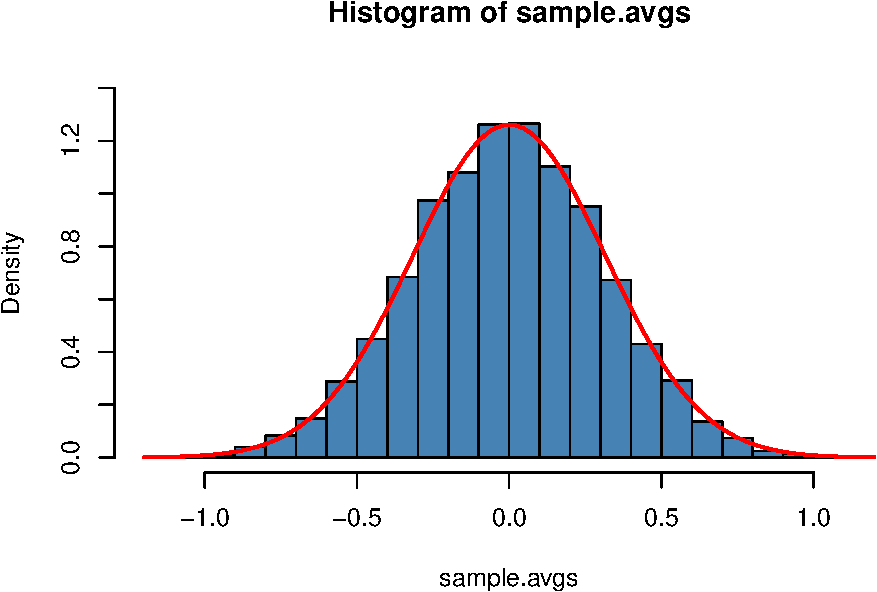
\includegraphics{URFITE_files/figure-latex/unnamed-chunk-45-1} \end{center}

\begin{Shaded}
\begin{Highlighting}[]
\CommentTok{# reproduce Figure 14.2 (b) of the book}
\KeywordTok{plot}\NormalTok{(}\KeywordTok{as.zoo}\NormalTok{(TSpread), }
     \DataTypeTok{col =} \StringTok{"steelblue"}\NormalTok{,}
     \DataTypeTok{lwd =} \DecValTok{2}\NormalTok{,}
     \DataTypeTok{xlab =} \StringTok{"Date"}\NormalTok{,}
     \DataTypeTok{ylab =} \StringTok{"Percent per annum"}\NormalTok{,}
     \DataTypeTok{main =} \StringTok{"Term Spread"}
\NormalTok{)}
\end{Highlighting}
\end{Shaded}

\begin{center}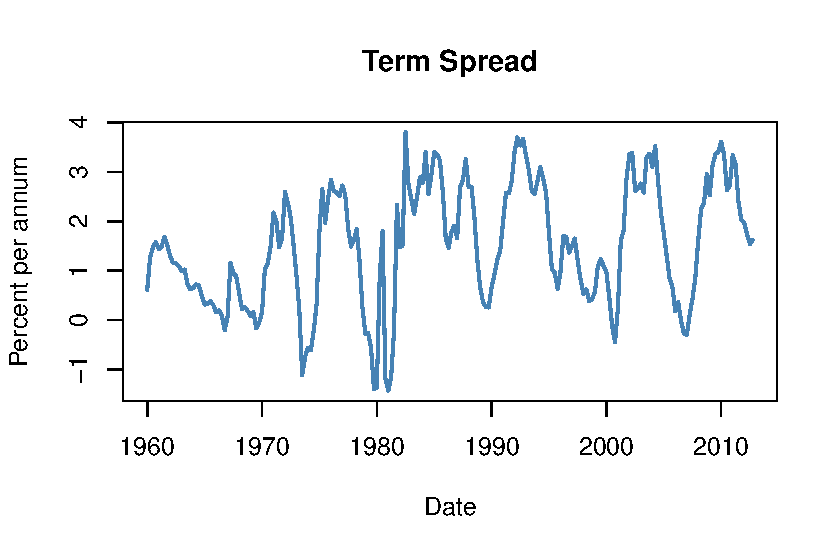
\includegraphics{URFITE_files/figure-latex/unnamed-chunk-45-2} \end{center}

Notice that before recessions, the gap between interests on long-term
bonds and short term bills narrows and consequently the term spread
declines drastically towards zero or even falls below zero in times of
economic stress. This information might be used to improve forecasts of
future GDP growth.

We check this by estimating an ADL(\(2\),\(1\)) model and an
ADL(\(2\),\(2\)) model of the GDP growth rate using lags of GDP growth
and lags of the term spread as regressors and use both models for
forecasting the GDP growth in 2013:Q1.

\begin{Shaded}
\begin{Highlighting}[]
\CommentTok{# convert growth and spread series to ts objects}
\NormalTok{GDPGrowth_ts <-}\StringTok{ }\KeywordTok{ts}\NormalTok{(GDPGrowth, }
                  \DataTypeTok{start =} \KeywordTok{c}\NormalTok{(}\DecValTok{1960}\NormalTok{, }\DecValTok{1}\NormalTok{), }
                  \DataTypeTok{end =} \KeywordTok{c}\NormalTok{(}\DecValTok{2013}\NormalTok{, }\DecValTok{4}\NormalTok{), }
                  \DataTypeTok{frequency =} \DecValTok{4}\NormalTok{)}

\NormalTok{TSpread_ts <-}\StringTok{ }\KeywordTok{ts}\NormalTok{(TSpread, }
                \DataTypeTok{start =} \KeywordTok{c}\NormalTok{(}\DecValTok{1960}\NormalTok{, }\DecValTok{1}\NormalTok{), }
                \DataTypeTok{end =} \KeywordTok{c}\NormalTok{(}\DecValTok{2012}\NormalTok{, }\DecValTok{4}\NormalTok{), }
                \DataTypeTok{frequency =} \DecValTok{4}\NormalTok{)}

\CommentTok{# join both ts objects}
\NormalTok{ADLdata <-}\StringTok{ }\KeywordTok{ts.union}\NormalTok{(GDPGrowth_ts, TSpread_ts)}
\end{Highlighting}
\end{Shaded}

\begin{Shaded}
\begin{Highlighting}[]
\CommentTok{# estimate the ADL(2,1) model of GDP growth}
\NormalTok{GDPGR_ADL21 <-}\StringTok{ }\KeywordTok{dynlm}\NormalTok{(GDPGrowth_ts }\OperatorTok{~}\StringTok{ }\KeywordTok{L}\NormalTok{(GDPGrowth_ts) }\OperatorTok{+}\StringTok{ }\KeywordTok{L}\NormalTok{(GDPGrowth_ts, }\DecValTok{2}\NormalTok{) }\OperatorTok{+}\StringTok{ }\KeywordTok{L}\NormalTok{(TSpread_ts), }
      \DataTypeTok{start =} \KeywordTok{c}\NormalTok{(}\DecValTok{1962}\NormalTok{, }\DecValTok{1}\NormalTok{), }\DataTypeTok{end =} \KeywordTok{c}\NormalTok{(}\DecValTok{2012}\NormalTok{, }\DecValTok{4}\NormalTok{))}

\KeywordTok{coeftest}\NormalTok{(GDPGR_ADL21, }\DataTypeTok{vcov. =}\NormalTok{ sandwich)}
\end{Highlighting}
\end{Shaded}

\begin{verbatim}
## 
## t test of coefficients:
## 
##                    Estimate Std. Error t value Pr(>|t|)   
## (Intercept)        0.954990   0.486976  1.9611 0.051260 . 
## L(GDPGrowth_ts)    0.267729   0.082562  3.2428 0.001387 **
## L(GDPGrowth_ts, 2) 0.192370   0.077683  2.4763 0.014104 * 
## L(TSpread_ts)      0.444047   0.182637  2.4313 0.015925 * 
## ---
## Signif. codes:  0 '***' 0.001 '**' 0.01 '*' 0.05 '.' 0.1 ' ' 1
\end{verbatim}

The estimated equation of the ADL(\(2\), \(1\)) model is

\begin{align}
  \widehat{GDPGR}_t = \underset{(0.49)}{0.96} + \underset{(0.08)}{0.26} GDPGR_{t-1} + \underset{(0.08)}{0.19} GDPGR_{t-2} + \underset{(0.18)}{0.44} TSpread_{t-1} \label{eq:gdpgradl21}
\end{align}

Notice that all coefficients are significant at the level of \(5\%\).

\begin{Shaded}
\begin{Highlighting}[]
\CommentTok{# 2012:Q3 / 2012:Q4 data on GDP growth and term spread}
\NormalTok{t <-}\StringTok{ }\KeywordTok{window}\NormalTok{(ADLdata, }\KeywordTok{c}\NormalTok{(}\DecValTok{2012}\NormalTok{, }\DecValTok{3}\NormalTok{), }\KeywordTok{c}\NormalTok{(}\DecValTok{2012}\NormalTok{, }\DecValTok{4}\NormalTok{))}

\CommentTok{# ADL(2,1) GDP growth forecast for 2013:Q1}
\NormalTok{ADL21_forecast <-}\StringTok{ }\KeywordTok{coef}\NormalTok{(GDPGR_ADL21) }\OperatorTok\StringTok{ }\KeywordTok{c}\NormalTok{(}\DecValTok{1}\NormalTok{, t[}\DecValTok{2}\NormalTok{, }\DecValTok{1}\NormalTok{], t[}\DecValTok{1}\NormalTok{, }\DecValTok{1}\NormalTok{], t[}\DecValTok{2}\NormalTok{, }\DecValTok{2}\NormalTok{])}
\NormalTok{ADL21_forecast}
\end{Highlighting}
\end{Shaded}

\begin{verbatim}
##          [,1]
## [1,] 2.241689
\end{verbatim}

\begin{Shaded}
\begin{Highlighting}[]
\CommentTok{# compute the forecast error}
\KeywordTok{window}\NormalTok{(GDPGrowth_ts, }\KeywordTok{c}\NormalTok{(}\DecValTok{2013}\NormalTok{, }\DecValTok{1}\NormalTok{), }\KeywordTok{c}\NormalTok{(}\DecValTok{2013}\NormalTok{, }\DecValTok{1}\NormalTok{)) }\OperatorTok{-}\StringTok{ }\NormalTok{ADL21_forecast}
\end{Highlighting}
\end{Shaded}

\begin{verbatim}
##           Qtr1
## 2013 -1.102487
\end{verbatim}

Model \eqref{eq:gdpgradl21} predicts the GDP growth in 2013:Q1 to be
\(2.24\%\) which leads to a forecast error of \(-1.10\%\).

We estimate the ADL(\(2\),\(2\)) specification to see whether adding
additional information on past term spread improves the forecast.

\begin{Shaded}
\begin{Highlighting}[]
\CommentTok{# estimate the ADL(2,2) model of GDP growth}
\NormalTok{GDPGR_ADL22 <-}\StringTok{ }\KeywordTok{dynlm}\NormalTok{(GDPGrowth_ts }\OperatorTok{~}\StringTok{ }\KeywordTok{L}\NormalTok{(GDPGrowth_ts) }\OperatorTok{+}\StringTok{ }\KeywordTok{L}\NormalTok{(GDPGrowth_ts, }\DecValTok{2}\NormalTok{) }
                     \OperatorTok{+}\StringTok{ }\KeywordTok{L}\NormalTok{(TSpread_ts) }\OperatorTok{+}\StringTok{ }\KeywordTok{L}\NormalTok{(TSpread_ts, }\DecValTok{2}\NormalTok{), }
                     \DataTypeTok{start =} \KeywordTok{c}\NormalTok{(}\DecValTok{1962}\NormalTok{, }\DecValTok{1}\NormalTok{), }\DataTypeTok{end =} \KeywordTok{c}\NormalTok{(}\DecValTok{2012}\NormalTok{, }\DecValTok{4}\NormalTok{))}

\KeywordTok{coeftest}\NormalTok{(GDPGR_ADL22, }\DataTypeTok{vcov. =}\NormalTok{ sandwich)}
\end{Highlighting}
\end{Shaded}

\begin{verbatim}
## 
## t test of coefficients:
## 
##                     Estimate Std. Error t value Pr(>|t|)   
## (Intercept)         0.967967   0.472470  2.0487 0.041800 * 
## L(GDPGrowth_ts)     0.243175   0.077836  3.1242 0.002049 **
## L(GDPGrowth_ts, 2)  0.177070   0.077027  2.2988 0.022555 * 
## L(TSpread_ts)      -0.139554   0.422162 -0.3306 0.741317   
## L(TSpread_ts, 2)    0.656347   0.429802  1.5271 0.128326   
## ---
## Signif. codes:  0 '***' 0.001 '**' 0.01 '*' 0.05 '.' 0.1 ' ' 1
\end{verbatim}

For the ADL(\(2\),\(2\)) model we obtain

\begin{align}
  \widehat{GDPGR}_t =& \, \underset{(0.47)}{0.98} + \underset{(0.08)}{0.24} GDPGR_{t-1} \\
                        +& \, \underset{(0.08)}{0.18} GDPGR_{t-2} + -\underset{(0.42)}{0.14} TSpread_{t-1} + \underset{(0.43)}{0.66} TSpread_{t-2}. \label{eq:gdpgradl22}
\end{align}

The coefficients on both lags of the term spread are not significant at
the \(10\%\) level.

\begin{Shaded}
\begin{Highlighting}[]
\CommentTok{# ADL(2,2) GDP growth forecast for 2013:Q1}
\NormalTok{ADL22_forecast <-}\StringTok{ }\KeywordTok{coef}\NormalTok{(GDPGR_ADL22) }\OperatorTok\StringTok{ }\KeywordTok{c}\NormalTok{(}\DecValTok{1}\NormalTok{, t[}\DecValTok{2}\NormalTok{, }\DecValTok{1}\NormalTok{], t[}\DecValTok{1}\NormalTok{, }\DecValTok{1}\NormalTok{], t[}\DecValTok{2}\NormalTok{, }\DecValTok{2}\NormalTok{], t[}\DecValTok{1}\NormalTok{, }\DecValTok{2}\NormalTok{])}
\NormalTok{ADL22_forecast}
\end{Highlighting}
\end{Shaded}

\begin{verbatim}
##          [,1]
## [1,] 2.274407
\end{verbatim}

\begin{Shaded}
\begin{Highlighting}[]
\CommentTok{# compute the forecast error}
\KeywordTok{window}\NormalTok{(GDPGrowth_ts, }\KeywordTok{c}\NormalTok{(}\DecValTok{2013}\NormalTok{, }\DecValTok{1}\NormalTok{), }\KeywordTok{c}\NormalTok{(}\DecValTok{2013}\NormalTok{, }\DecValTok{1}\NormalTok{)) }\OperatorTok{-}\StringTok{ }\NormalTok{ADL22_forecast}
\end{Highlighting}
\end{Shaded}

\begin{verbatim}
##           Qtr1
## 2013 -1.135206
\end{verbatim}

The ADL(\(2\),\(2\)) forecast of GDP growth in 2013:Q1 is \(2.27\%\)
which imples a forecast error of \(1.14\%\).

Do the ADL models \eqref{eq:gdpgradl21} and \eqref{eq:gdpgradl22} improve
upon the simple AR(\(2\)) model \eqref{eq:GDPGRAR2} in terms of
forecasting GPD growth in 2013:Q1? The answer is yes: while \(SER\) and
\(\overline{R}^2\) improve only slightly, an \(F\)-test on the term
spread coefficients in \eqref{eq:gdpgradl22} provides evidence that the
model does better in explaining GPD growth than the AR(\(2\)) model as
the hypothesis that both coefficients are zero cannot be rejected at the
level of \(5\%\).

\begin{Shaded}
\begin{Highlighting}[]
\CommentTok{# compare adj. R2}
\KeywordTok{c}\NormalTok{(}
  \StringTok{"Adj.R2 AR(2)"}\NormalTok{ =}\StringTok{ }\KeywordTok{summary}\NormalTok{(GDPGR_AR2)}\OperatorTok{$}\NormalTok{r.squared,}
  \StringTok{"Adj.R2 ADL(2,1)"}\NormalTok{ =}\StringTok{ }\KeywordTok{summary}\NormalTok{(GDPGR_ADL21)}\OperatorTok{$}\NormalTok{r.squared,}
  \StringTok{"Adj.R2 ADL(2,2)"}\NormalTok{ =}\StringTok{ }\KeywordTok{summary}\NormalTok{(GDPGR_ADL22)}\OperatorTok{$}\NormalTok{r.squared}
\NormalTok{)}
\end{Highlighting}
\end{Shaded}

\begin{verbatim}
##    Adj.R2 AR(2) Adj.R2 ADL(2,1) Adj.R2 ADL(2,2) 
##       0.1425484       0.1743996       0.1855245
\end{verbatim}

\begin{Shaded}
\begin{Highlighting}[]
\CommentTok{# compare SER}
\KeywordTok{c}\NormalTok{(}
  \StringTok{"SER AR(2)"}\NormalTok{ =}\StringTok{ }\KeywordTok{summary}\NormalTok{(GDPGR_AR2)}\OperatorTok{$}\NormalTok{sigma,}
  \StringTok{"SER ADL(2,1)"}\NormalTok{ =}\StringTok{ }\KeywordTok{summary}\NormalTok{(GDPGR_ADL21)}\OperatorTok{$}\NormalTok{sigma,}
  \StringTok{"SER ADL(2,2)"}\NormalTok{ =}\StringTok{ }\KeywordTok{summary}\NormalTok{(GDPGR_ADL22)}\OperatorTok{$}\NormalTok{sigma}
\NormalTok{)}
\end{Highlighting}
\end{Shaded}

\begin{verbatim}
##    SER AR(2) SER ADL(2,1) SER ADL(2,2) 
##     3.132122     3.070760     3.057655
\end{verbatim}

\begin{Shaded}
\begin{Highlighting}[]
\CommentTok{# F-test on coefficients of term spread}
\KeywordTok{linearHypothesis}\NormalTok{(GDPGR_ADL22, }
                 \KeywordTok{c}\NormalTok{(}\StringTok{"L(TSpread_ts)=0"}\NormalTok{, }\StringTok{"L(TSpread_ts, 2)=0"}\NormalTok{),}
                 \DataTypeTok{vcov. =}\NormalTok{ sandwich}
\NormalTok{                 )}
\end{Highlighting}
\end{Shaded}

\begin{verbatim}
## Linear hypothesis test
## 
## Hypothesis:
## L(TSpread_ts) = 0
## L(TSpread_ts, 2) = 0
## 
## Model 1: restricted model
## Model 2: GDPGrowth_ts ~ L(GDPGrowth_ts) + L(GDPGrowth_ts, 2) + L(TSpread_ts) + 
##     L(TSpread_ts, 2)
## 
## Note: Coefficient covariance matrix supplied.
## 
##   Res.Df Df      F  Pr(>F)  
## 1    201                    
## 2    199  2 4.4344 0.01306 *
## ---
## Signif. codes:  0 '***' 0.001 '**' 0.01 '*' 0.05 '.' 0.1 ' ' 1
\end{verbatim}

\subsubsection*{Stationarity}\label{stationarity}
\addcontentsline{toc}{subsubsection}{Stationarity}

In general, forecasts an be improved by using mutliple predictors ---
just as in cross-sectional regression. For time series regressions to
yield reliable models, the assumption of \emph{stationarity} must be
fulfilled. Key Concept 14.5 explains what stationarity is.

Key Concept 14.5

Stationarity

We say that a time series \(Y_t\) is stationary if its probability
distribution is time independent, that is the joint distribution of
\(Y_{s+1}, Y_{s+2},\dots,Y_{s+T}\) does not change as \(s\) is varied,
regardless of \(T\).

Similarly, we say that two time series \(X_t\) and \(Y_t\) are
\emph{jointly stationary} if the joint distribution of
\((X_{s+1},Y_{s+1}, X_{s+2},Y_{s+2} \dots, X_{s+T}Y_{s+T})\) does not
depend on \(s\), regardless of \(T\).

In a probabilistic sense, stationarity means that information about how
a time series evolves in the future is inherent to its past. If this is
not the case, we cannot use the past of a series as a reliable guideline
for its future.

\subsubsection*{Time Series Regression with Multiple
Predictors}\label{time-series-regression-with-multiple-predictors}
\addcontentsline{toc}{subsubsection}{Time Series Regression with
Multiple Predictors}

The concept of stationarity is a key assumption in the general time
series regression model with multiple predictors. Key Concept 14.6
elaborates this model and its assumptions.

Key Concept 14.6

Time Series Regression with Multiple Predictors

The general time series regression model extends the ADL such that
multiple regressors and their lags are included. It uses \(p\) lags of
the dependent variable and \(q_l\) lags of \(l\) additional predictors
where \(l=1,\dots,k\):

\begin{equation}
  \begin{aligned}
  Y_t =& \, \beta_0 + \beta_1 Y_{t-1} + \beta_2 Y_{t-2} + \dots + \beta_{p} Y_{t-p} \\
      +& \, \delta_{11} X_{1,t-1} + \delta_{12} X_{1,t-2} + \dots + \delta_{1q} X_{1,t-q} \\
      +& \, \dots \\
      +& \, \delta_{k1} X_{k,t-1} + \delta_{k2} X_{k,t-2} + \dots + \delta_{kq} X_{k,t-q} \\
      +& \, u_t 
\end{aligned}
\end{equation}

For estimation we make the following assumptions:

\begin{enumerate}
\def\labelenumi{\arabic{enumi}.}
\item
  The error term \(u_t\) has conditional mean zero given all regressors
  and their lags:
  \[E(u_t\vert Y_{t-1}, Y_{t-2}, \dots, X_{1,t-1}, X_{1,t-2} \dots, X_{k,t-1}, X_{k,t-2}, \dots)\]
  This assumption is an extension of the conditional mean zero
  assumption used for AR and ADL models and guarantees that the general
  time series regression model stated above gives the best forecast of
  \(Y_t\) given its lags, the additional regressors
  \(X_{1,t},\dots,X_{k,t}\) and their lags.
\item
  The \(i.i.d\) assumption for cross-sectional data is not (entirely)
  meaningful for time series data. We replace it by the following
  assumption witch consists of two parts:

  \begin{enumerate}
  \def\labelenumii{(\alph{enumii})}
  \item
    The \((Y_{t}, X_{1,t}, \dots, X_{k,t})\) have a stationary
    distribution (the ``identically distributed'' part of the i.i.d.
    assumption for cross-setional data). If this does not hold,
    forecasts may be biased and inference can be strongly misleading.
  \item
    \((Y_{t}, X_{1,t}, \dots, X_{k,t})\) and
    \((Y_{t-j}, X_{1,t-j}, \dots, X_{k,t-j})\) become independent as
    \(j\) gets large (the ``idependly'' distributed part of the i.i.d.
    assumption for cross-sectional data). This assumption is also called
    \emph{weak dependence}. It ensures that the WLLN and the CLT hold in
    large samples.
  \end{enumerate}
\item
  Large outliers are unlikely:
  \(E(X_{1,t}^4), E(X_{2,t}^4), \dots, E(X_{k,t}^4)\) and \(E(Y_t^4)\)
  have nonzero, finite fourth moments.
\item
  No perfect multicollinearity.
\end{enumerate}

Since many economic time series appear to be nonstationary, assumption
two of Key Concept 14.6 is a crucial one in applied macroeconomics and
finance which is why statistical test for stationarity / nonstationarity
have been developed. Chapters 14.6 and 14.7 are devoted to this topic.

\subsubsection*{Statistical inference and the Granger causality
test}\label{statistical-inference-and-the-granger-causality-test}
\addcontentsline{toc}{subsubsection}{Statistical inference and the
Granger causality test}

If a \(X\) is a useful predictor for \(Y\), in a regression of \(Y_t\)
on lags of its own and lags of \(X_t\), not all of the coefficients on
the lags on \(X_t\) are zero. This concept is called ``Granger
causality'' and is an interesting hypothesis to test. Key Concept 14.7
summarizes the idea.

Key Concept 14.7

Granger Causality Tests

The Granger causality test (Granger, 1969) is an \(F\)-test of the null
hypothesis that \emph{all} lags of a variable \(X\) included in a time
series regression model do not have predictive power for \(Y_t\). The
Granger causality test does not test whether \(X\) actually
\emph{causes} \(Y\) but whether the included lags are informative in
terms of predicting \(Y\).

Notice that we have already performed a Granger causality test on the
coefficients of term spread in \eqref{eq:gdpgradl22}, the ADL(\(2\),\(2\))
model of GDP growth and concluded that at least one of the first two
lags of term spread has predictive power for GDP growth.

\subsection*{Forecast Uncertainty and Forecast
Intervals}\label{forecast-uncertainty-and-forecast-intervals}
\addcontentsline{toc}{subsection}{Forecast Uncertainty and Forecast
Intervals}

In general, it is a good practice to report a measure of the uncertainty
inherent to the estimation. Uncertainty is particulary of interest when
forecasting a time series. For example, consider a simple ADL\((1,1)\)
model

\begin{align*}
  Y_t = \beta_0 + \beta_1 Y_{t-1} + \delta_1 X_{t-1} + u_t
\end{align*}

where \(u_t\) is a homoskedastic error term. The forecast error is

\begin{align*}
  Y_{T+1} - \widehat{Y}_{T+1\vert T} = u_{T+1} - \left[(\widehat{\beta}_0 - \beta_0) + (\widehat{\beta}_1 - \beta_1) Y_T + (\widehat{\delta_1} - \delta_1) X_t \right].
\end{align*}

The mean squared forecast error (MSFE) and the RMFSE are

\begin{align*}
  MFSE =& \, E\left[(Y_{T+1} - \widehat{Y}_{T+1\vert T})^2 \right] \\
       =& \, \sigma_u^2 + Var\left[ (\widehat{\beta}_0 - \beta_0) + (\widehat{\beta}_1 - \beta_1) Y_T + (\widehat{\delta_1} - \delta_1) X_t \right], \\
  RMFSE =& \, \sqrt{\sigma_u^2 + Var\left[ (\widehat{\beta}_0 - \beta_0) + (\widehat{\beta}_1 - \beta_1) Y_T + (\widehat{\delta_1} - \delta_1) X_t \right]}.
\end{align*}

A \(95\%\) forecast interval is an interval that covers the true value
of \(Y_{T+1}\) in \(95\%\) of repeated applications. Note that there is
a major difference in computing a confidence interval and a forecast
interval: when computing a confidence interval of a point estimate we
use large sample approximations that are justified by the CLT and thus
are valid for a large range of error term distributions. For computation
of a forecast interval of \(Y_{T+1}\), however, we must make an
additional assumption about the distribution of \(u_{T+1}\), the error
term in period \(T+1\). Assuming that \(u_{T+1}\) is normally
distributed one can construct a \(95\%\) \emph{forecast interval} for
\(Y_{T+1}\) using \(SE(Y_{T+1} - \widehat{Y}_{T+1\vert T})\), an
estimate of the RMSFE:

\begin{align*}
  \widehat{Y}_{T+1\vert T} \pm 1.96 \cdot SE(Y_{T+1} - \widehat{Y}_{T+1\vert T})
\end{align*}

Of course the computation gets more complicated when the error term is
heteroskedastic or if we are interested in computing a forecast interval
for \(T+s, s>1\).

In some applications it is useful to report multiple forecast intervals
for each step in range of subsequents periods, see the Box \emph{The
River of Blood} on p.~592 of the book. Such forecast ranges can be
visualized in a so-called fan chart. We will not replicate the fan chart
presented in Figure 14.2 of book because the underlying model is by far
more complex than the simple AR and ADL models treated here. Instead, in
the example below we use simulated time series data and estimate an
ADL(\(1\),\(1\)) model which is then used for forecasting the subsequent
25 future outcomes of the series. We choose
\texttt{level\ =\ seq(5,99,10)} in the call of \texttt{forecast()} such
that forecast intervals with levels \(5\%, 15\%, \dots, 95\%\) are
computed for each point forecast of the series.

\begin{Shaded}
\begin{Highlighting}[]
\CommentTok{# simulate the time series}
\KeywordTok{set.seed}\NormalTok{(}\DecValTok{1234}\NormalTok{)}

\NormalTok{Z <-}\StringTok{ }\KeywordTok{arima.sim}\NormalTok{(}\KeywordTok{list}\NormalTok{(}\DataTypeTok{order =} \KeywordTok{c}\NormalTok{(}\DecValTok{1}\NormalTok{, }\DecValTok{0}\NormalTok{, }\DecValTok{0}\NormalTok{), }\DataTypeTok{ar =} \FloatTok{0.5}\NormalTok{),  }\DataTypeTok{n =} \DecValTok{200}\NormalTok{)}
\NormalTok{X <-}\StringTok{ }\KeywordTok{arima.sim}\NormalTok{(}\KeywordTok{list}\NormalTok{(}\DataTypeTok{order =} \KeywordTok{c}\NormalTok{(}\DecValTok{1}\NormalTok{, }\DecValTok{0}\NormalTok{, }\DecValTok{0}\NormalTok{), }\DataTypeTok{ar =} \FloatTok{0.2}\NormalTok{),  }\DataTypeTok{n =} \DecValTok{200}\NormalTok{)}

\NormalTok{Y <-}\StringTok{ }\FloatTok{0.7} \OperatorTok{*}\StringTok{ }\NormalTok{Z }\OperatorTok{+}\StringTok{ }\FloatTok{0.7} \OperatorTok{*}\StringTok{ }\NormalTok{X }\OperatorTok{+}\StringTok{ }\KeywordTok{rnorm}\NormalTok{(}\DecValTok{100}\NormalTok{)}

\CommentTok{# estimate an ADL(1,1) model using arima, see ?arima}
\NormalTok{model <-}\StringTok{ }\KeywordTok{arima}\NormalTok{(Y, }\DataTypeTok{order =} \KeywordTok{c}\NormalTok{(}\DecValTok{2}\NormalTok{, }\DecValTok{0}\NormalTok{, }\DecValTok{0}\NormalTok{))}

\CommentTok{# compute points forecasts and prediction intervals for the next 25 periods}
\NormalTok{fc <-}\StringTok{ }\KeywordTok{forecast}\NormalTok{(model, }\DataTypeTok{h =} \DecValTok{25}\NormalTok{, }\DataTypeTok{level =} \KeywordTok{seq}\NormalTok{(}\DecValTok{5}\NormalTok{, }\DecValTok{99}\NormalTok{, }\DecValTok{10}\NormalTok{))}

\CommentTok{# plot a fan chart}
\KeywordTok{plot}\NormalTok{(fc, }
     \DataTypeTok{main =} \StringTok{"Forecast Fan Chart for ADL(2,2) Model of Simulated Data"}\NormalTok{, }
     \DataTypeTok{showgap =}\NormalTok{ F, }
     \DataTypeTok{fcol =} \StringTok{"red"}\NormalTok{,}
     \DataTypeTok{flty =} \DecValTok{2}\NormalTok{)}
\end{Highlighting}
\end{Shaded}

\begin{center}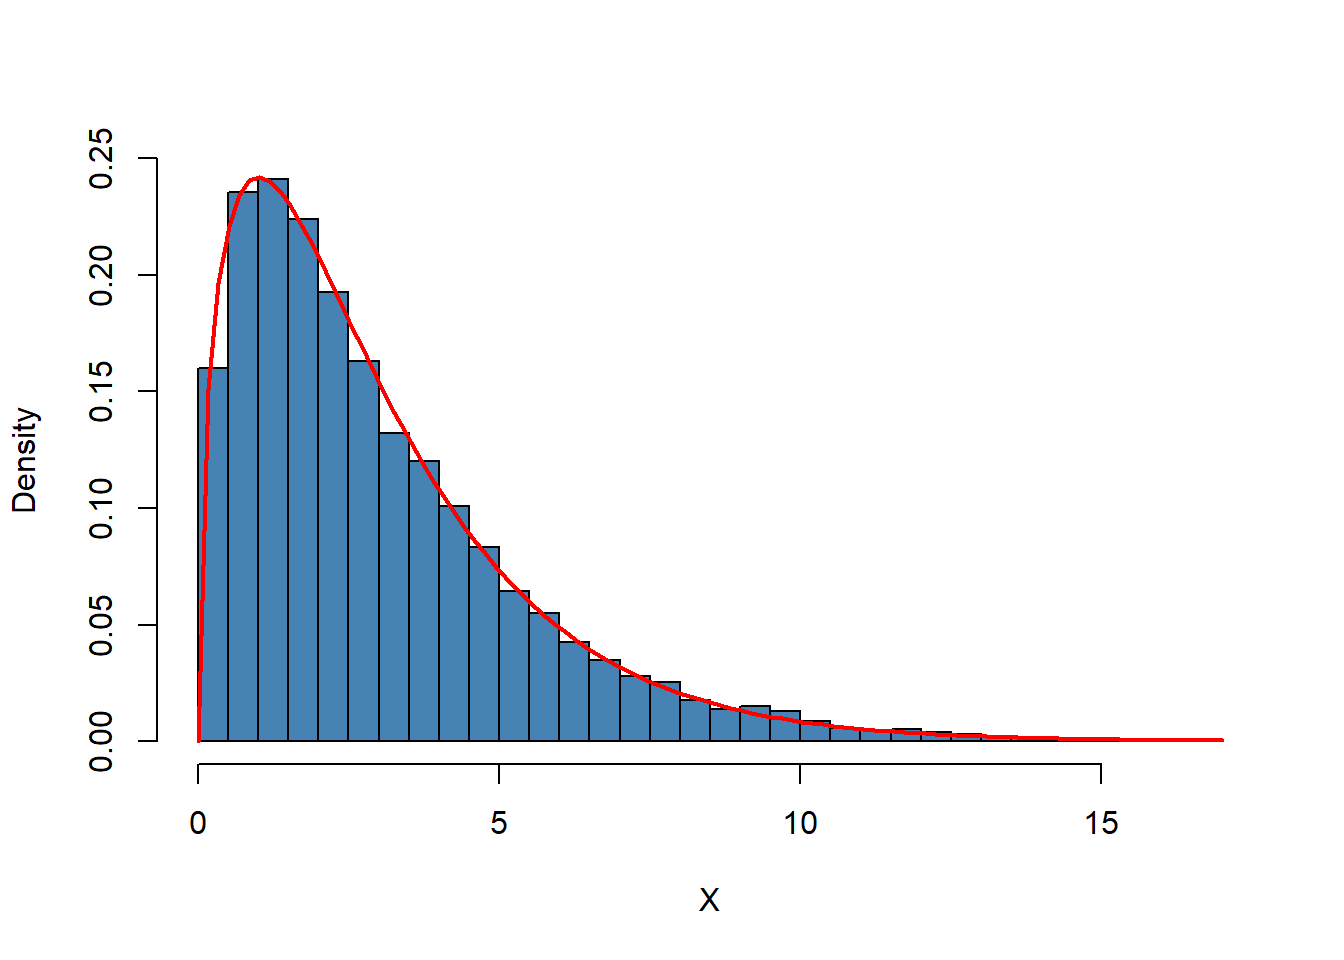
\includegraphics{URFITE_files/figure-latex/unnamed-chunk-52-1} \end{center}

The dashed red line shows point forecasts of the series for the next 25
periods based on an \(ADL(1,1)\) model and the shaded areas represent
the prediction intervals. The degree of shading indicates the level of
the prediction interval. The darkest of the blue bands displays the
\(5\%\) forecast intervals and the color fades towards grey as the level
of the intervals increases.

\section{Lag Length Selection Using Information
Criteria}\label{lag-length-selection-using-information-criteria}

The selection of lag lengths in AR and ADL models can be partially
governed by economic theory. However, there are statistical methods that
are helpful to determine how many lags should be included as regressors.
In general, to many lags inflate the standard errors of coefficient
estimates and thus imply an increase in the forecast error while
omitting lags that should be included in the model may result in an
estimation bias.

The order of an AR model can be determined using two approaches

\begin{enumerate}
\def\labelenumi{\arabic{enumi}.}
\item
  ** The \(F\)-test approach**:

  Estimate an AR(\(p\)) model and test the significance of the largest
  lag(s). If the test rejects, drop the respective lag(s) from the
  model. This approach has the tendency to produce models where the
  order is too large: in a significance test we always face the risk of
  rejecting a true null hypothesis!
\item
  \textbf{Relying on an information criterion}:

  To circumvent the issue of producing too large models, one may choose
  the lag order that minimizes one of the following two information
  criteria:

  \begin{itemize}
  \item
    The \emph{Bayes information criterion} (BIC):

    \[BIC(p) = \log\left(\frac{SSR(p)}{T}\right) + (p + 1) \frac{\log(T)}{T}\]
  \item
    The \emph{Akaike information criterion} (AIC):

    \[AIC(p) = \log\left(\frac{SSR(p)}{T}\right) + (p + 1) \frac{2}{T}\]
  \end{itemize}

  Both criteria are estimators of the optimal lag length \(p\). The lag
  order \(\widehat{p}\) that minimizes the respective criterion is
  called the \emph{BIC estimate} or the \emph{AIC estimate} of the
  optimal model order. The basic idea of both criteria is that the
  \(SSR\) decreases as additional lags are added to the model such that
  the first addend decreases wheras the second addend increases as the
  lag order grows. One can show that the the \(BIC\) is a consistent
  estimator of the true lag order while the AIC is not which is due to
  the differing factors in the second addend. Nevertheless, both
  estimators are used in practice where the \(AIC\) is sometimes used as
  an alternative when the \(BIC\) yields a model with too few lags.
\end{enumerate}

The function\texttt{dynlm()} does not compute informatoin criteria by
default. We will therefore write a short function that reports the
\(BIC\) (along with the chosen lag order \(p\) and \(R^2\)) for objects
of class \texttt{dynlm}.

\begin{Shaded}
\begin{Highlighting}[]
\CommentTok{# compute BIC for AR model objects of class `dynlm` }
\NormalTok{BIC <-}\StringTok{ }\ControlFlowTok{function}\NormalTok{(model) \{}
  
\NormalTok{  ssr <-}\StringTok{ }\KeywordTok{sum}\NormalTok{(model}\OperatorTok{$}\NormalTok{residuals}\OperatorTok{^}\DecValTok{2}\NormalTok{)}
\NormalTok{  t <-}\StringTok{ }\KeywordTok{length}\NormalTok{(model}\OperatorTok{$}\NormalTok{residuals)}
\NormalTok{  npar <-}\StringTok{ }\KeywordTok{length}\NormalTok{(model}\OperatorTok{$}\NormalTok{coef)}
  
  \KeywordTok{return}\NormalTok{(}
    \KeywordTok{round}\NormalTok{(}
      \KeywordTok{c}\NormalTok{(}
      \StringTok{"p"}\NormalTok{ =}\StringTok{ }\NormalTok{npar }\OperatorTok{-}\StringTok{ }\DecValTok{1}\NormalTok{,}
      \StringTok{"BIC"}\NormalTok{ =}\StringTok{ }\KeywordTok{log}\NormalTok{(ssr}\OperatorTok{/}\NormalTok{t) }\OperatorTok{+}\StringTok{ }\NormalTok{npar }\OperatorTok{*}\StringTok{ }\KeywordTok{log}\NormalTok{(t)}\OperatorTok{/}\NormalTok{t,}
      \StringTok{"R2"}\NormalTok{ =}\StringTok{ }\KeywordTok{summary}\NormalTok{(model)}\OperatorTok{$}\NormalTok{r.squared}
\NormalTok{      ), }\DecValTok{4}
\NormalTok{    )}
\NormalTok{  )}
  
\NormalTok{\}}
\end{Highlighting}
\end{Shaded}

Table 14.3 of the book presents a breakdown of how the \(BIC\) is
computed for AR(\(p\)) models of GDP growth with order \(p=1,\dots,6\).
The final result can easily be reproduced using \texttt{sapply()} and
the function \texttt{BIC()} defined above.

\begin{Shaded}
\begin{Highlighting}[]
\CommentTok{# apply the BIC() to an intercept only model of GDP growth}
\KeywordTok{BIC}\NormalTok{(}
  \KeywordTok{dynlm}\NormalTok{(}\KeywordTok{ts}\NormalTok{(GDPGR_leads) }\OperatorTok{~}\StringTok{ }\DecValTok{1}\NormalTok{)}
\NormalTok{)}
\end{Highlighting}
\end{Shaded}

\begin{verbatim}
##      p    BIC     R2 
## 0.0000 2.4394 0.0000
\end{verbatim}

\begin{Shaded}
\begin{Highlighting}[]
\CommentTok{# loop BIC over models of different orders}
\NormalTok{order <-}\StringTok{ }\DecValTok{1}\OperatorTok{:}\DecValTok{6}

\NormalTok{BICs <-}\StringTok{ }\KeywordTok{sapply}\NormalTok{(order, }
       \ControlFlowTok{function}\NormalTok{(x) }
        \StringTok{"AR"}\NormalTok{ =}\StringTok{ }\KeywordTok{BIC}\NormalTok{(}
          \KeywordTok{dynlm}\NormalTok{(}\KeywordTok{ts}\NormalTok{(GDPGR_leads) }\OperatorTok{~}\StringTok{ }\KeywordTok{L}\NormalTok{(}\KeywordTok{ts}\NormalTok{(GDPGR_leads), }\DecValTok{1}\OperatorTok{:}\NormalTok{x))}
\NormalTok{          )}
\NormalTok{       )}

\NormalTok{BICs}
\end{Highlighting}
\end{Shaded}

\begin{verbatim}
##       [,1]   [,2]   [,3]   [,4]   [,5]   [,6]
## p   1.0000 2.0000 3.0000 4.0000 5.0000 6.0000
## BIC 2.3486 2.3475 2.3774 2.4034 2.4188 2.4429
## R2  0.1143 0.1425 0.1434 0.1478 0.1604 0.1591
\end{verbatim}

Note that increasing the lag order increases \(R^2\) because the \(SSR\)
decreases as additional lags are added to the model but according to the
\(BIC\), we should decide for the AR(\(2\)) model instead of the
AR(\(6\)) model. It helps to decide whether the decrease in \(SSR\) is
enough to justify adding an additional regressor.

If we would have to compare a bigger set of models, a convenient way to
select the model with the lowest \(BIC\) is using the function
\texttt{which.min()}

\begin{Shaded}
\begin{Highlighting}[]
\CommentTok{# select the AR model with the smallest BIC}
\NormalTok{BICs[, }\KeywordTok{which.min}\NormalTok{(BICs[}\DecValTok{2}\NormalTok{, ])]}
\end{Highlighting}
\end{Shaded}

\begin{verbatim}
##      p    BIC     R2 
## 2.0000 2.3475 0.1425
\end{verbatim}

The \(BIC\) may also be used to select lag lengths in time series
regression models with multiple predictors. In a model with \(K\)
coefficients, including the intercept, we have

\begin{align*}
    BIC(K) = \log\left(\frac{SSR(K)}{T}\right) + K \frac{\log(T)}{T}.
\end{align*}

Notice that choosing the optimal model according to the \(BIC\) can be
computationally demaning because there may be many different
combinations of lag lengths when there are multiple predictors.

To motivate an example, we estimate ADL(\(p\),\(q\)) models of GDP
growth where, as above, the additional variable is the term spread
between short-term and long-term bonds. We impose the restriction that
\(p=q_1=\dots=q_k\) so that only \(p_{max}\) models
(\(p=1,\dots,p_{max}\)) need to be estimated. In the example below we
choose \(p_{max} = 12\).

\begin{Shaded}
\begin{Highlighting}[]
\CommentTok{# loop BIC over ADL models }
\NormalTok{order <-}\StringTok{ }\DecValTok{1}\OperatorTok{:}\DecValTok{12}

\NormalTok{BICs <-}\StringTok{ }\KeywordTok{sapply}\NormalTok{(order, }
       \ControlFlowTok{function}\NormalTok{(x) }
         \KeywordTok{BIC}\NormalTok{(}
          \KeywordTok{dynlm}\NormalTok{(GDPGrowth_ts }\OperatorTok{~}\StringTok{ }\KeywordTok{L}\NormalTok{(GDPGrowth_ts, }\DecValTok{1}\OperatorTok{:}\NormalTok{x) }\OperatorTok{+}\StringTok{ }\KeywordTok{L}\NormalTok{(TSpread_ts, }\DecValTok{1}\OperatorTok{:}\NormalTok{x), }
          \DataTypeTok{start =} \KeywordTok{c}\NormalTok{(}\DecValTok{1962}\NormalTok{, }\DecValTok{1}\NormalTok{), }\DataTypeTok{end =} \KeywordTok{c}\NormalTok{(}\DecValTok{2012}\NormalTok{, }\DecValTok{4}\NormalTok{))}
\NormalTok{          )}
\NormalTok{       )}

\NormalTok{BICs}
\end{Highlighting}
\end{Shaded}

\begin{verbatim}
##       [,1]   [,2]   [,3]   [,4]    [,5]    [,6]    [,7]    [,8]    [,9]
## p   2.0000 4.0000 6.0000 8.0000 10.0000 12.0000 14.0000 16.0000 18.0000
## BIC 2.3411 2.3408 2.3813 2.4181  2.4568  2.5048  2.5539  2.6029  2.6182
## R2  0.1417 0.1855 0.1950 0.2072  0.2178  0.2211  0.2234  0.2253  0.2581
##       [,10]   [,11]   [,12]
## p   20.0000 22.0000 24.0000
## BIC  2.6646  2.7205  2.7664
## R2   0.2678  0.2702  0.2803
\end{verbatim}

Notice that from the definition of \texttt{BIC()}, for ADL models with
\(p=q\) it follows that p reports the number of estimated coefficients
\emph{excluding} the intercept. Thus the lag order is obtained by
deviding p by 2.

\begin{Shaded}
\begin{Highlighting}[]
\CommentTok{# select the ADL model with the smallest BIC}
\NormalTok{BICs[, }\KeywordTok{which.min}\NormalTok{(BICs[}\DecValTok{2}\NormalTok{, ])]}
\end{Highlighting}
\end{Shaded}

\begin{verbatim}
##      p    BIC     R2 
## 4.0000 2.3408 0.1855
\end{verbatim}

The \(BIC\) is in favour of the ADL(\(2\),\(2\)) model
\eqref{eq:gdpgradl22} we have estimated before.

\section{Nonstationarity I: Trends}\label{nonstationarity-i-trends}

If a series is nonstationary, conventional hypothesis tests, confidence
intervals and forecasts can be strongly misleading. The assumption of
stationarity is violated if a series exhibits trends or breaks and the
resulting complications in an econometric analysis depend on the
specific type of the nonstationarity. This section focuses on time
series that exhibit trends.

A series is said to exhibit a trend if it fluctuates around a persistent
long-term movement. One distinguishes between \emph{deterministic} and
\emph{stochastic} trends.

\begin{itemize}
\item
  We say that a trend is \emph{deterministic} if it is a nonrandom
  function of time.
\item
  A trend is said to be \emph{stochastic} if it is a random function of
  time.
\end{itemize}

A careful look at the figures we have produced in Chapter 14.2 reveals
that many economic time series show a trending behaviour that is
probably best modeled by stochastic trends. This is why the book focuses
on the treatment of stochastic trends.

\subsubsection*{The Random Walk Model of a
Trend}\label{the-random-walk-model-of-a-trend}
\addcontentsline{toc}{subsubsection}{The Random Walk Model of a Trend}

The simplest way to model a time series \(Y_t\) that has stochastic
trend is the \emph{random walk}

\begin{align}
  Y_t = Y_{t-1} + u_t, \label{eq:randomwalk}
\end{align}

where the \(u_t\) are i.i.d. errors with
\(E(u_t\vert Y_{t-1}, Y_{t-2}, \dots) = 0\). Note that

\begin{align*}
  E(Y_t\vert Y_{t-1}, Y_{t-2}\dots) =& \, E(Y_{t-1}\vert Y_{t-1}, Y_{t-2}\dots) + E(u_t\vert Y_{t-1}, Y_{t-2}\dots) \\
  =& \, Y_{t-1}
\end{align*}

so the best forecast for \(Y_t\), todays value of \(Y\), is \(Y_{t-1}\),
the observation made yesterday so the difference between \(Y_t\) and
\(Y_{t-1}\) is unpredictable. One can shows that the path followed by
\(Y_t\) consists of random steps \(u_t\), hence it is called a random
walk.

Assume that \(Y_0\), the starting value of the random walk is \(0\).
Another way to write out \eqref{eq:randomwalk} is

\begin{align*}
  Y_0 =& \, 0 \\
  Y_1 =& \, 0 + u_1 \\
  Y_2 =& \, 0 + u_1 + u_2 \\
  \vdots & \, \\
  Y_t =& \, \sum_{i=1}^t u_i.
\end{align*}

Therefore we have

\begin{align*}
  var(Y_t) =& \, Var(u_1 + u_2 + \dots + u_t) \\
           =& \, t \sigma_u^2.
\end{align*}

Thus the variance of a random walk depends on \(t\) which violates the
assumption presented in Key Concept 14.5: a random walk is
nonstationary.

Obviously, \eqref{eq:randomwalk} is a special case of an AR(\(1\)) model
where \(\beta_1 = 1\). One can show that a time series that follows an
AR(\(1\)) model is stationary if \(\lvert\beta_1\rvert < 1\). In a
general AR(\(p\)) model, stationarity is linked to the roots of the
polynomial
\[1-\beta_1 z - \beta_2 z^2 - \beta_3 z^3 - \dots - \beta_p z^p.\] If
all roots are greater than \(1\) in absolute value, the AR(\(p\)) series
is stationary. If at least one root equals \(1\), the AR(\(p\)) is said
to have a \emph{unit root} and thus has a stochastic trend.

It is straightforward to simulate random walks in R using
\texttt{arima.sim()}. The function \texttt{matplot()} is covenient for
simple plots of the columns of a matrix.

\begin{Shaded}
\begin{Highlighting}[]
\CommentTok{# simulate and plot random walks starting at 0}
\KeywordTok{set.seed}\NormalTok{(}\DecValTok{1}\NormalTok{)}

\NormalTok{RWs <-}\StringTok{ }\KeywordTok{ts}\NormalTok{(}
  \KeywordTok{replicate}\NormalTok{(}\DataTypeTok{n =} \DecValTok{4}\NormalTok{, }
            \KeywordTok{arima.sim}\NormalTok{(}\DataTypeTok{model =} \KeywordTok{list}\NormalTok{(}\DataTypeTok{order =} \KeywordTok{c}\NormalTok{(}\DecValTok{0}\NormalTok{, }\DecValTok{1}\NormalTok{ ,}\DecValTok{0}\NormalTok{)), }\DataTypeTok{n =} \DecValTok{100}\NormalTok{)}
\NormalTok{            )}
\NormalTok{  )}

\KeywordTok{matplot}\NormalTok{(RWs, }
        \DataTypeTok{type =}\StringTok{"l"}\NormalTok{, }
        \DataTypeTok{col =} \KeywordTok{c}\NormalTok{(}\StringTok{"steelblue"}\NormalTok{, }\StringTok{"darkgreen"}\NormalTok{, }\StringTok{"darkred"}\NormalTok{, }\StringTok{"orange"}\NormalTok{), }
        \DataTypeTok{lty =} \DecValTok{1}\NormalTok{, }
        \DataTypeTok{lwd =} \DecValTok{2}\NormalTok{,}
        \DataTypeTok{main =} \StringTok{"Four Random Walks"}\NormalTok{,}
        \DataTypeTok{xlab =} \StringTok{"Time"}\NormalTok{,}
        \DataTypeTok{ylab =} \StringTok{"Value"}
\NormalTok{        )}
\end{Highlighting}
\end{Shaded}

\begin{center}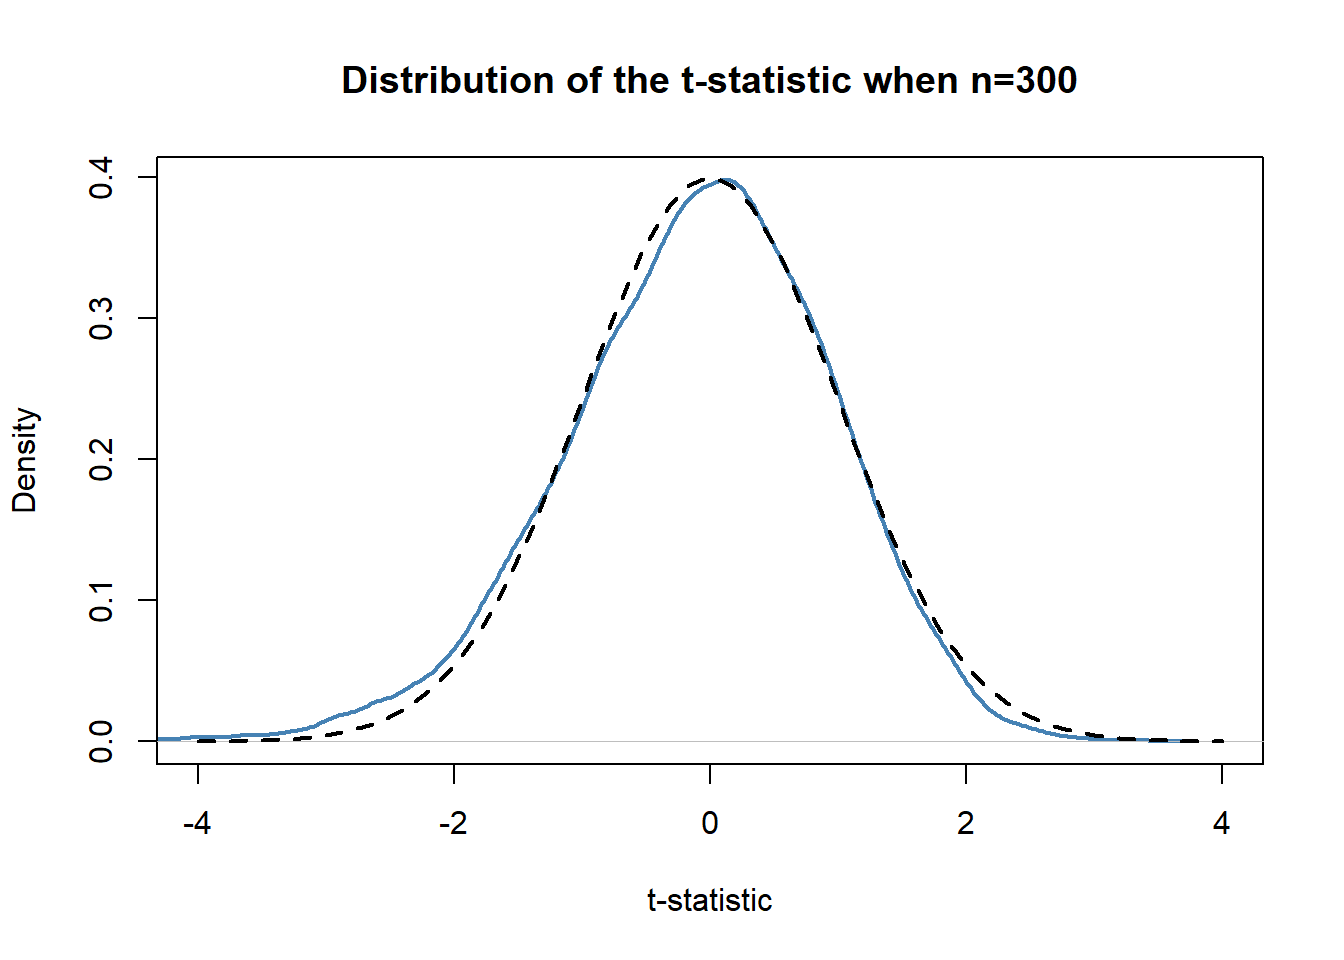
\includegraphics{URFITE_files/figure-latex/unnamed-chunk-58-1} \end{center}

Adding a constant to \eqref{eq:randomwalk} yields

\begin{align}
  Y_t = \beta_0 + Y_{t-1} + u_t \label{eq:randomwalkdrift},
\end{align}

a \emph{random walk model with a drift} which allows to model the
tendency of a series to move in one direction or the other. If
\(\beta_0\) is positive, the series drifts upwards and it follows a
downward trend if \(\beta_0\) is negative.

\begin{Shaded}
\begin{Highlighting}[]
\CommentTok{# simulate and plot random walks with drift starting at 0 }
\KeywordTok{set.seed}\NormalTok{(}\DecValTok{1}\NormalTok{)}

\NormalTok{RWsd <-}\StringTok{ }\KeywordTok{ts}\NormalTok{(}
  \KeywordTok{replicate}\NormalTok{(}\DataTypeTok{n =} \DecValTok{4}\NormalTok{, }
            \KeywordTok{arima.sim}\NormalTok{(}\DataTypeTok{model =} \KeywordTok{list}\NormalTok{(}\DataTypeTok{order =} \KeywordTok{c}\NormalTok{(}\DecValTok{0}\NormalTok{, }\DecValTok{1}\NormalTok{, }\DecValTok{0}\NormalTok{)), }\DataTypeTok{n =} \DecValTok{100}\NormalTok{)}
\NormalTok{            )}
\NormalTok{  )}

\KeywordTok{matplot}\NormalTok{(RWsd, }
        \DataTypeTok{type=}\StringTok{"l"}\NormalTok{, }
        \DataTypeTok{col =} \KeywordTok{c}\NormalTok{(}\StringTok{"steelblue"}\NormalTok{, }\StringTok{"darkgreen"}\NormalTok{, }\StringTok{"darkred"}\NormalTok{, }\StringTok{"orange"}\NormalTok{), }
        \DataTypeTok{lty =} \DecValTok{1}\NormalTok{, }
        \DataTypeTok{lwd =} \DecValTok{2}\NormalTok{,}
        \DataTypeTok{main =} \StringTok{"Four Random Walks with Drift"}\NormalTok{,}
        \DataTypeTok{xlab =} \StringTok{"Time"}\NormalTok{,}
        \DataTypeTok{ylab =} \StringTok{"Value"}
\NormalTok{        )}
\end{Highlighting}
\end{Shaded}

\begin{center}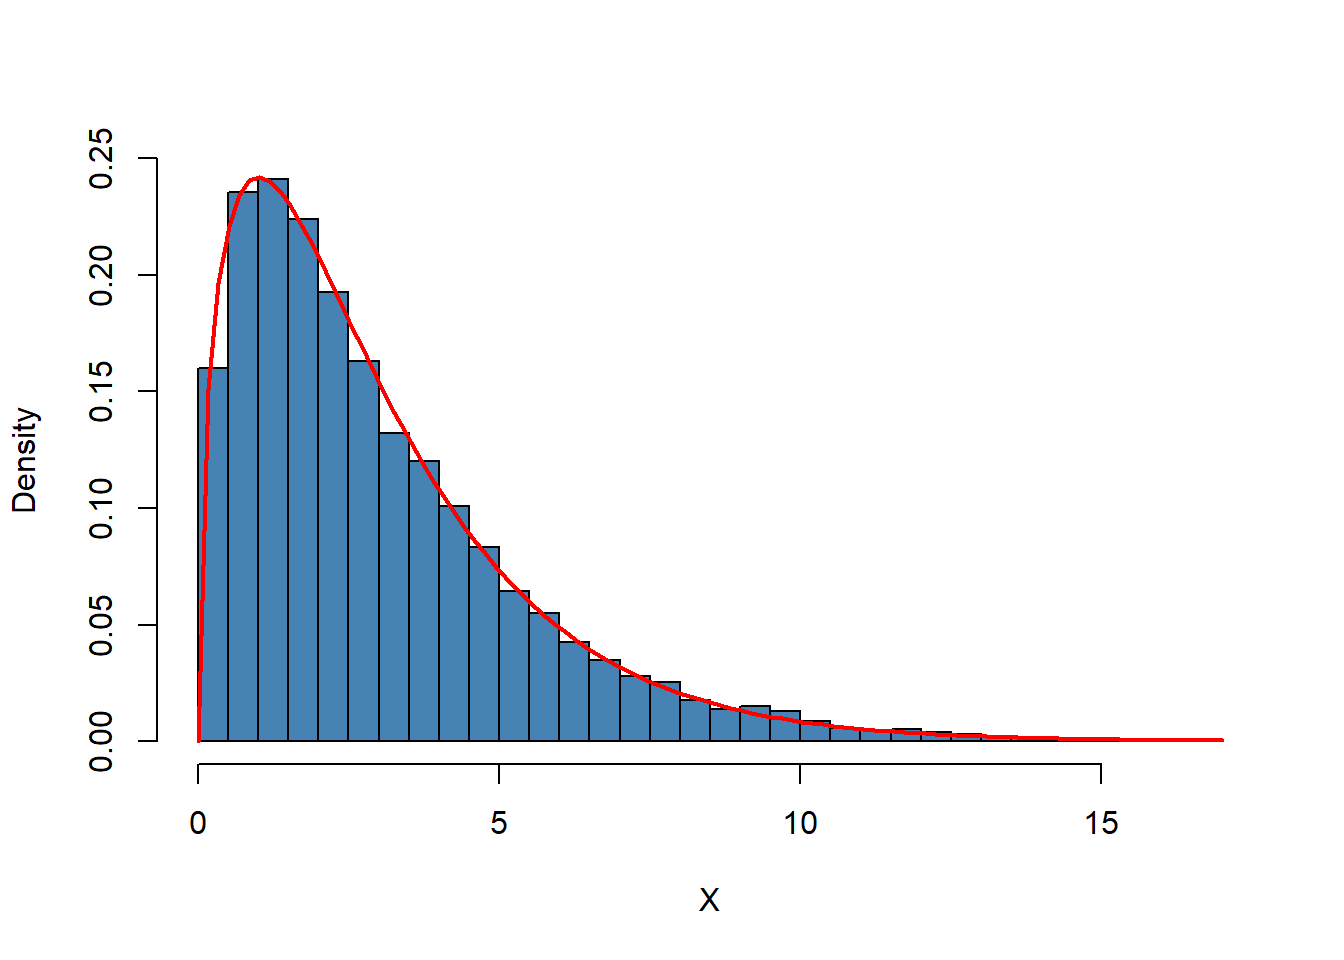
\includegraphics{URFITE_files/figure-latex/unnamed-chunk-59-1} \end{center}

\textless{}7div\textgreater{}

\subsubsection*{Problems Caused by Stochastic
Trends}\label{problems-caused-by-stochastic-trends}
\addcontentsline{toc}{subsubsection}{Problems Caused by Stochastic
Trends}

OLS estimation of the coefficients on regressors that have a stochastic
trend is problematic because the distribution of the estimator and its
\(t\)-statistic is nonnormal, even asymptotically. This has various
consequences:

\begin{itemize}
\item
  Downward bias of autoregressive coefficients:

  If \(Y_t\) is a random walk, the coefficient \(\beta_1\) can be
  consistently estimated by OLS but the estimator is biased toward zero.
  This bias is roughly \(E(\widehat{\beta}_1) = 1 - 5.3/T\) which is
  substantial for sample sizes typically encountered in macroeconomics.
  This estimation bias causes forecasts of \(Y_t\) to perform worse than
  a pure random walk model.
\item
  Nonnormally distributed \(t\)-statistics:

  The nonnormal distribution of the estimated coefficient of a
  stochastic regressor translates to a nonnormal distribution of its
  \(t\)-statistic so that normal critical values are invalid and
  therefore usual confidence intervals and hypothesis tests are invalid,
  too, and the true distribution of the \(t\)-statistic cannot be
  readily determined.
\item
  Spurious Regression:

  When a time series that exhibits a stochastic trend is regressed on
  another time series that does have a stochastic trend too, the
  estimated relationship may appear highly significant although the
  series are unrelated. This is what econometricians call a
  \emph{spurious} relationship.
\end{itemize}

As an example for spurious regression, consider again the green and the
red random walks that we have simulated above. We know that there is no
relationship between both series: they are purely random and independent
of each other.

\begin{Shaded}
\begin{Highlighting}[]
\CommentTok{# plot spurious relationship}
\KeywordTok{matplot}\NormalTok{(RWs[, }\KeywordTok{c}\NormalTok{(}\DecValTok{2}\NormalTok{, }\DecValTok{3}\NormalTok{)], }
        \DataTypeTok{lty =} \DecValTok{1}\NormalTok{,}
        \DataTypeTok{lwd =} \DecValTok{2}\NormalTok{,}
        \DataTypeTok{type =} \StringTok{"l"}\NormalTok{,}
        \DataTypeTok{col =} \KeywordTok{c}\NormalTok{(}\StringTok{"darkgreen"}\NormalTok{, }\StringTok{"darkred"}\NormalTok{),}
        \DataTypeTok{xlab =} \StringTok{"Time"}\NormalTok{,}
        \DataTypeTok{ylab =} \StringTok{""}\NormalTok{,}
        \DataTypeTok{main =} \StringTok{"A Spurious Relationship"}
\NormalTok{        )    }
\end{Highlighting}
\end{Shaded}

\begin{center}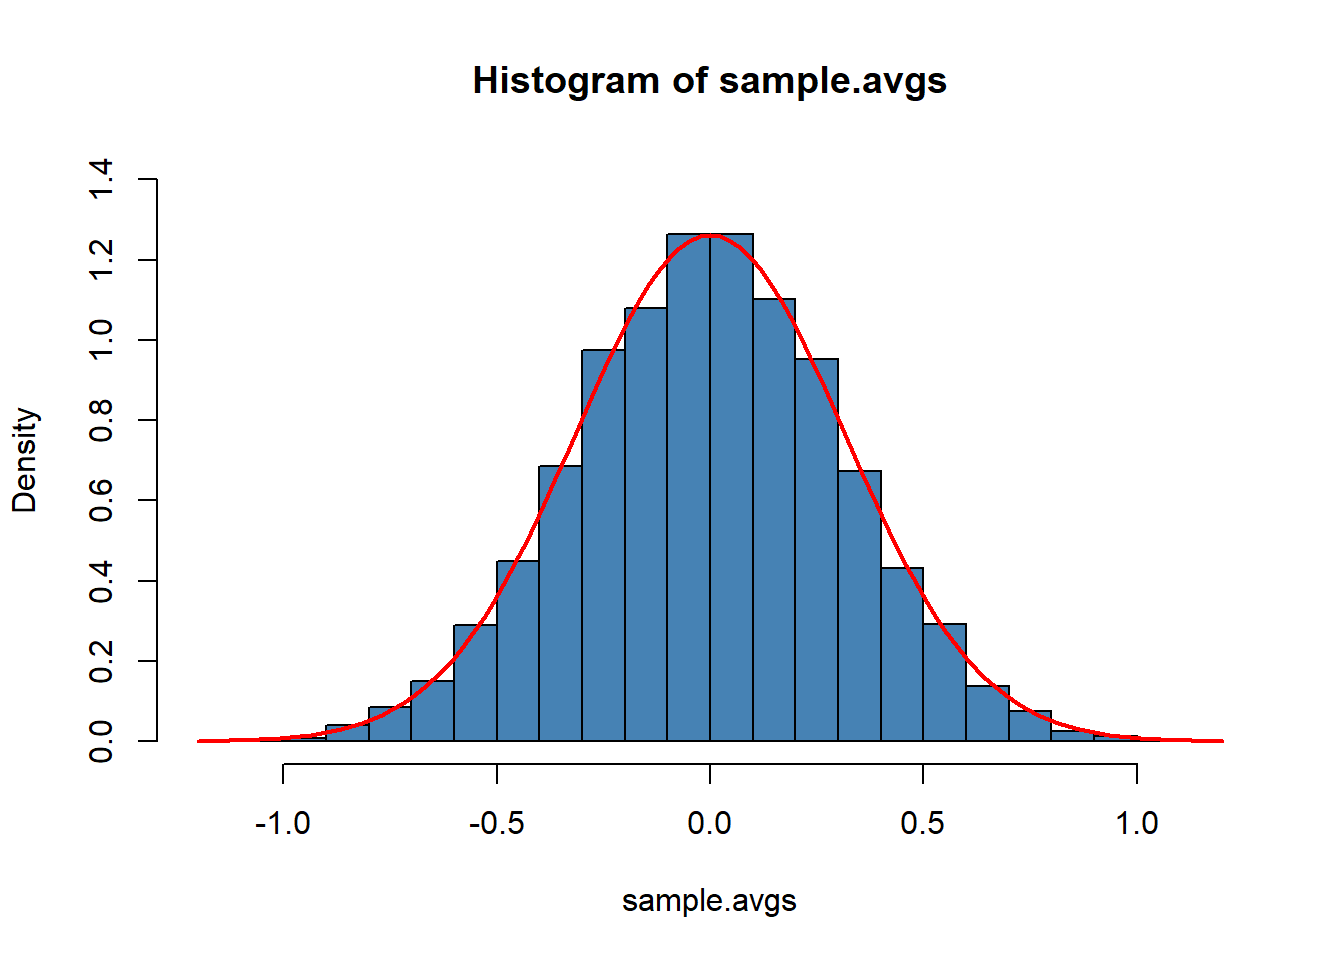
\includegraphics{URFITE_files/figure-latex/unnamed-chunk-60-1} \end{center}

Imagine we did not have this information and instead conject that the
green series is useful for predicting the red series and thus end up
estimating the ADL(\(0\),\(1\)) model

\begin{align*}
  Red_t = \beta_0 + \beta_1 Green_{t-1} + u_t.
\end{align*}

\begin{Shaded}
\begin{Highlighting}[]
\CommentTok{# estimate spurious AR model}
\KeywordTok{summary}\NormalTok{(}
  \KeywordTok{dynlm}\NormalTok{(RWs[, }\DecValTok{2}\NormalTok{] }\OperatorTok{~}\StringTok{ }\KeywordTok{L}\NormalTok{(RWs[, }\DecValTok{3}\NormalTok{]))}
\NormalTok{  )}\OperatorTok{$}\NormalTok{coefficients}
\end{Highlighting}
\end{Shaded}

\begin{verbatim}
##              Estimate Std. Error   t value     Pr(>|t|)
## (Intercept) -3.459488  0.3635104 -9.516889 1.354156e-15
## L(RWs[, 3])  1.047195  0.1450874  7.217687 1.135828e-10
\end{verbatim}

The result is obviously spurious: the coefficient on \(Green_{t-1}\) is
estimated to be about \(1\) and the \(p\)-value of
\(1.14 \cdot 10^{-10}\) of the corresponding \(t\)-test indicates that
the coefficient is highly significant while its true value is in fact
zero.

As an empirical example, consider the U.S. unemployment rate and the
Japanese industrial production. Both series show an upward trending
behaviour from the mid-1960s through the early 1980s.

\begin{Shaded}
\begin{Highlighting}[]
\CommentTok{# Plot U.S. unemployment rate & Japanese industrial production}
\KeywordTok{plot}\NormalTok{(}\KeywordTok{merge}\NormalTok{(}\KeywordTok{as.zoo}\NormalTok{(USUnemp), }\KeywordTok{as.zoo}\NormalTok{(JPIndProd)), }
     \DataTypeTok{plot.type =} \StringTok{"single"}\NormalTok{, }
     \DataTypeTok{col =} \KeywordTok{c}\NormalTok{(}\StringTok{"darkred"}\NormalTok{, }\StringTok{"steelblue"}\NormalTok{),}
     \DataTypeTok{lwd =} \DecValTok{2}\NormalTok{,}
     \DataTypeTok{xlab =} \StringTok{"Date"}\NormalTok{,}
     \DataTypeTok{ylab =} \StringTok{""}\NormalTok{,}
     \DataTypeTok{main =} \StringTok{"Spurious Regression: Macroeconomic Time series"}
\NormalTok{)}
\KeywordTok{legend}\NormalTok{(}\StringTok{"topleft"}\NormalTok{, }
       \DataTypeTok{legend =} \KeywordTok{c}\NormalTok{(}\StringTok{"USUnemp"}\NormalTok{,}\StringTok{"JPIndProd"}\NormalTok{),}
       \DataTypeTok{col =} \KeywordTok{c}\NormalTok{(}\StringTok{"darkred"}\NormalTok{, }\StringTok{"steelblue"}\NormalTok{),}
       \DataTypeTok{lwd =} \KeywordTok{c}\NormalTok{(}\DecValTok{2}\NormalTok{, }\DecValTok{2}\NormalTok{)}
\NormalTok{       )}
\end{Highlighting}
\end{Shaded}

\begin{center}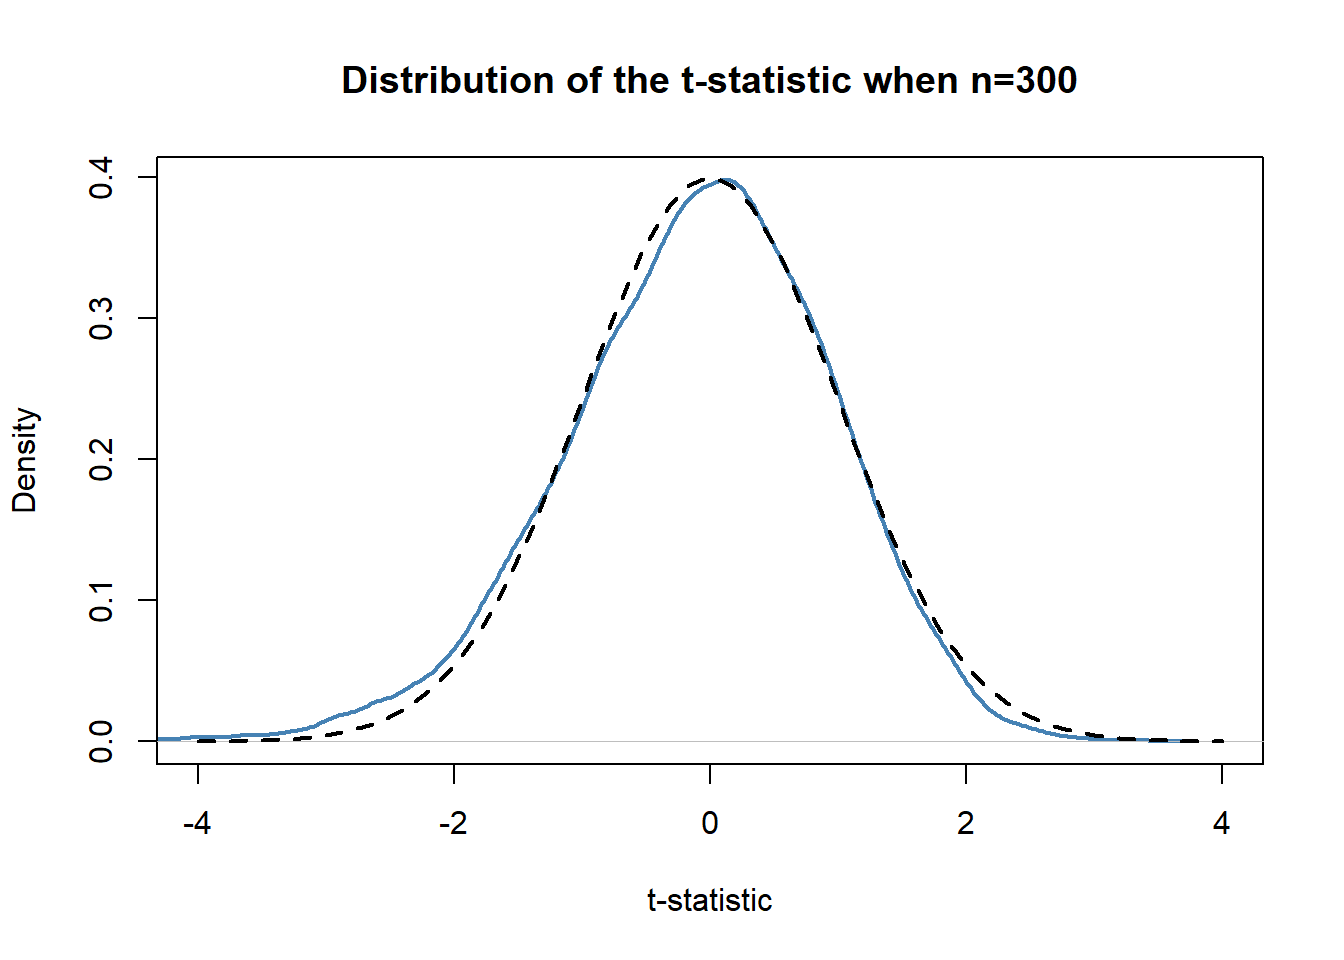
\includegraphics{URFITE_files/figure-latex/unnamed-chunk-62-1} \end{center}

\begin{Shaded}
\begin{Highlighting}[]
\CommentTok{# Estimate regression using data from 1962 to 1985}
\NormalTok{SR_Unemp1 <-}\StringTok{ }\KeywordTok{dynlm}\NormalTok{(}\KeywordTok{ts}\NormalTok{(USUnemp[}\StringTok{"1962::1985"}\NormalTok{]) }\OperatorTok{~}\StringTok{ }\KeywordTok{ts}\NormalTok{(JPIndProd[}\StringTok{"1962::1985"}\NormalTok{]))}
\KeywordTok{coeftest}\NormalTok{(SR_Unemp1, }\DataTypeTok{vcov =}\NormalTok{ sandwich)}
\end{Highlighting}
\end{Shaded}

\begin{verbatim}
## 
## t test of coefficients:
## 
##                             Estimate Std. Error t value  Pr(>|t|)    
## (Intercept)                 -2.37452    1.12041 -2.1193    0.0367 *  
## ts(JPIndProd["1962::1985"])  2.22057    0.29233  7.5961 2.227e-11 ***
## ---
## Signif. codes:  0 '***' 0.001 '**' 0.01 '*' 0.05 '.' 0.1 ' ' 1
\end{verbatim}

A simple regression of the U.S. unemployment rate on Japanese industrial
production using data from 1962 to 1985 yields

\begin{align}
  \widehat{U.S. UR}_t = -\underset{(1.12)}{2.37} + \underset{(0.29)}{2.22} \log(JapaneseIP_t). \label{eq:urjpip1}
\end{align}

This appears to be a significant relationship: the \(t\)-statistic of
the coefficient on \(\log(JapaneseIP_t)\) is bigger than 7.

\begin{Shaded}
\begin{Highlighting}[]
\CommentTok{# Estimate regression using data from 1986 to 2012}
\NormalTok{SR_Unemp2 <-}\StringTok{ }\KeywordTok{dynlm}\NormalTok{(}\KeywordTok{ts}\NormalTok{(USUnemp[}\StringTok{"1986::2012"}\NormalTok{]) }\OperatorTok{~}\StringTok{ }\KeywordTok{ts}\NormalTok{(JPIndProd[}\StringTok{"1986::2012"}\NormalTok{]))}
\KeywordTok{coeftest}\NormalTok{(SR_Unemp2, }\DataTypeTok{vcov =}\NormalTok{ sandwich)}
\end{Highlighting}
\end{Shaded}

\begin{verbatim}
## 
## t test of coefficients:
## 
##                             Estimate Std. Error t value  Pr(>|t|)    
## (Intercept)                  41.7763     5.4066  7.7270 6.596e-12 ***
## ts(JPIndProd["1986::2012"])  -7.7771     1.1714 -6.6391 1.386e-09 ***
## ---
## Signif. codes:  0 '***' 0.001 '**' 0.01 '*' 0.05 '.' 0.1 ' ' 1
\end{verbatim}

When estimating the same model, this time with data from 1986 to 2012,
we obtain

\begin{align}
  \widehat{U.S. UR}_t = \underset{(5.41)}{41.78} + \underset{(1.17)}{-7.78} \log(JapaneseIP)_t \label{eq:urjpip2}
\end{align}

which is suprisingly quite different from \eqref{eq:urjpip1} which
indicates a moderate postive relationship, in contrast to the large
negative coefficient in \eqref{eq:urjpip2}. This phenomenon can be
attributed to stochastic trends in the series: since there is no
economic reasoning that relates both trends, both regressions are
spurious.

\subsubsection*{Testing for a Unit AR
Root}\label{testing-for-a-unit-ar-root}
\addcontentsline{toc}{subsubsection}{Testing for a Unit AR Root}

A formal test for a stochastic trend has been proposed by Dickey and
Fuller (1979) and is therefore termend the \emph{Dickey-Fuller test}. As
discussed above, a time series that follows an AR(\(1\)) model with
\(\beta_1 = 1\) has a stochastic trend. Thus, the testing problem is

\begin{align*}
  H_0: \beta_1 = 1 \ \ \ \text{vs.} \ \ \ H_1: \beta_1 < 1.
\end{align*}

The null hypothesis is that the AR(\(1\)) has a unit root and the
alternative hypothesis is that it is stationary. One often rewrites the
AR(\(1\)) by substracting \(Y_{t-1}\) on both sides:

\begin{align*}
  Y_t = \beta_0 + \beta_1 Y_{t-1} + u_t \ \ \Leftrightarrow \ \ \Delta Y_t = \beta_0 + \delta_1 Y_{t-1} + u_i
\end{align*}

where \(\delta_1 = \beta_1 - 1\). The testing problem then becomes

\begin{align*}
  H_0: \delta_1 = 0 \ \ \ \text{vs.} \ \ \ H_1: \beta_1 < 0
\end{align*}

which is convenient since the corresponding test statistic is reported
by many relevant R functions.\footnote{The \(t\)-statistic of the
  Dickey-Fuller test is computed using homoskedasticity-only standard
  errors since under the null hypothesis, the usual \(t\)-statistic is
  robust to heteroskedasticity.}

The Dickey-Fuller test can also be applied in an AR(\(p\)) model. The
\emph{Augmented Dickey-Fuller (ADF) test} is summarized in Key Concept
14.8.

Key Concept 14.8

The ADF Test for a Unit Root

Consider the regression

\begin{align}
  \Delta Y_t = \beta_0 + \delta Y_{t-1} + \gamma_1 \Delta_1 Y_{t-1} + \gamma_2 \Delta Y_{t-2} + \dots + \gamma_p \Delta Y_{t-p} + u_t. \label{eq:ADFreg1}
\end{align}

The ADF test for a unit autoregressive root tests the hypothesis
\(H_0: \delta = 0\) (stochastic trend) against the one-sided alternative
\(H_1: \delta < 0\) (stationarity) using the usual OLS \(t\)-statistic.

If it is assumed that \(Y_t\) is stationary around a deterministic
linear time trend, the model is augmented by the regressor \(t\), that
is \(Y_t\) becomes

\begin{align}
  \Delta Y_t = \beta_0 + at + \delta Y_{t-1} + \gamma_1 \Delta_1 Y_{t-1} + \gamma_2 \Delta Y_{t-2} + \dots + \gamma_p \Delta Y_{t-p} + u_t,  \label{eq:ADFreg2}
\end{align}

where again \(H_0: \delta = 0\) is tested against \(H_1: \delta < 0\).

The optimal lag length \(p\) can be estimated using information
criteria. Notice that in the regression \eqref{eq:ADFreg1}, \(p=0\) (that
is no lags of \(\Delta Y_t\) are used as regressors) corresponds to a
simple AR(\(1\)).

Under the null hypothesis, the \(t\)-statistic corresponding to
\(H_0: \delta = 0\) does not have a normal distribution. The cricital
values can only be obtained from simulation and differ for regressions
\eqref{eq:ADFreg1} and \eqref{eq:ADFreg2} since the distribution of the ADF
test statistic is sensitive to the deterministic components included in
the regression.

\subsubsection*{Critical Values for the ADF
Statistic}\label{critical-values-for-the-adf-statistic}
\addcontentsline{toc}{subsubsection}{Critical Values for the ADF
Statistic}

Key Concept 14.8 states that the critical values for the ADF test in the
regressions \eqref{eq:ADFreg1} and \eqref{eq:ADFreg2} can only be determined
using simulation. The idea of the simulation study is to simulate a
large number of ADF test test statistics and use them to estimate
quantiles of their \emph{asymptotic} distribution. This section shows
how this is feasible whithin R.

First, consider an AR(\(1\)) model with drift. The procedure is as
follows:

\begin{itemize}
\item
  Simulate \(N\) random walks with \(n\) observations using the data
  generating process

  \begin{align*}
    Y_t =& \, \beta_0 + \beta_1 Y_{t-1} + u_t,
  \end{align*}

  \(t=1,\dots,n\) where \(N\) and \(n\) are large numbers.
\item
  For each random walk, estimate the regression

  \begin{align*}
    \Delta Y_t =& \, \beta_0 + \beta_1 Y_{t-1} + u_t
  \end{align*}

  and compute ADF test statistic. Save all \(N\) test statistics in a
  vector.
\item
  Estimate quantiles of the distribution of the ADF test statistic using
  the \(N\) test statistics obtained from the simulation.
\end{itemize}

For the case with drift and linear time trend we replace the data
generating process by

\begin{align*}
  Y_t =& \, \beta_0 + \alpha t + \beta_1 Y_{t-1} + u_t
\end{align*}

and estimate

\begin{align*}
  \Delta Y_t =& \, \beta_0 + \alpha t + \beta_1 Y_{t-1} + u_t.
\end{align*}

Loosely speaking, the precision of the estimated quantiles depends on
two factors: \(n\), the length of the underlying series and \(N\), the
number of test statistics used. Since we are interested in estimating
quantiles of the \emph{asymptotic} distribution (the Dickey-Fuller
distribution) of the ADF test statistic so both using many observations
and large number of simulated test statistics will increase the
precision of the estimated quantiles. We choose \(n=N=1000\) as the
computational burden grows quickly with \(n\) and \(N\).

\begin{Shaded}
\begin{Highlighting}[]
\CommentTok{# repititions}
\NormalTok{N <-}\StringTok{ }\DecValTok{1000}

\CommentTok{# observations}
\NormalTok{n <-}\StringTok{ }\DecValTok{1000}

\CommentTok{# define drift a trend }
\NormalTok{drift <-}\StringTok{ }\FloatTok{0.5}
\NormalTok{trend <-}\StringTok{ }\DecValTok{1}\OperatorTok{:}\NormalTok{n}

\CommentTok{# simulate N random walks with drift }
\NormalTok{RWD <-}\StringTok{ }\KeywordTok{ts}\NormalTok{(}\KeywordTok{replicate}\NormalTok{(}\DataTypeTok{n =}\NormalTok{ N, }
\NormalTok{            drift }\OperatorTok{+}\StringTok{ }\KeywordTok{arima.sim}\NormalTok{(}\DataTypeTok{model =} \KeywordTok{list}\NormalTok{(}\DataTypeTok{order =} \KeywordTok{c}\NormalTok{(}\DecValTok{0}\NormalTok{, }\DecValTok{1}\NormalTok{, }\DecValTok{0}\NormalTok{)),}
                              \DataTypeTok{n =}\NormalTok{ n }\OperatorTok{-}\StringTok{ }\DecValTok{1}\NormalTok{)}
\NormalTok{            )}
\NormalTok{          )}

\CommentTok{# compute ADF test statistics and store them in 'ADFD'}
\NormalTok{ADFD <-}\StringTok{ }\KeywordTok{numeric}\NormalTok{(N)}

\ControlFlowTok{for}\NormalTok{(i }\ControlFlowTok{in} \DecValTok{1}\OperatorTok{:}\KeywordTok{ncol}\NormalTok{(RWD)) \{}
\NormalTok{  ADFD[i] <-}\StringTok{ }\KeywordTok{summary}\NormalTok{(}
    \KeywordTok{dynlm}\NormalTok{(}\KeywordTok{diff}\NormalTok{(RWD[, i], }\DecValTok{1}\NormalTok{) }\OperatorTok{~}\StringTok{ }\KeywordTok{L}\NormalTok{(RWD[, i], }\DecValTok{1}\NormalTok{))}
\NormalTok{    )}\OperatorTok{$}\NormalTok{coef[}\DecValTok{2}\NormalTok{, }\DecValTok{3}\NormalTok{]}
\NormalTok{\}}

\CommentTok{# simulate N random walks with drift + trend}
\NormalTok{RWDT <-}\StringTok{ }\KeywordTok{ts}\NormalTok{(}\KeywordTok{replicate}\NormalTok{(}\DataTypeTok{n =}\NormalTok{ N, }
\NormalTok{                    trend }\OperatorTok{+}\StringTok{ }\NormalTok{drift }\OperatorTok{+}\StringTok{ }\KeywordTok{arima.sim}\NormalTok{(}\DataTypeTok{model =} \KeywordTok{list}\NormalTok{(}\DataTypeTok{order =} \KeywordTok{c}\NormalTok{(}\DecValTok{0}\NormalTok{, }\DecValTok{1}\NormalTok{, }\DecValTok{0}\NormalTok{)), }
                                              \DataTypeTok{n =}\NormalTok{ n }\OperatorTok{-}\StringTok{ }\DecValTok{1}\NormalTok{)}
\NormalTok{                    )}
\NormalTok{           )}

\CommentTok{# compute ADF test statistics and store them in 'ADFDT'}
\NormalTok{ADFDT <-}\StringTok{ }\KeywordTok{numeric}\NormalTok{(N)}

\ControlFlowTok{for}\NormalTok{(i }\ControlFlowTok{in} \DecValTok{1}\OperatorTok{:}\KeywordTok{ncol}\NormalTok{(RWDT)) \{}
\NormalTok{  ADFDT[i] <-}\StringTok{ }\KeywordTok{summary}\NormalTok{(}
    \KeywordTok{dynlm}\NormalTok{(}\KeywordTok{diff}\NormalTok{(RWDT[, i], }\DecValTok{1}\NormalTok{) }\OperatorTok{~}\StringTok{ }\KeywordTok{L}\NormalTok{(RWDT[, i], }\DecValTok{1}\NormalTok{) }\OperatorTok{+}\StringTok{ }\KeywordTok{trend}\NormalTok{(RWDT[, i], }\DataTypeTok{scale =}\NormalTok{ F))}
\NormalTok{  )}\OperatorTok{$}\NormalTok{coef[}\DecValTok{2}\NormalTok{, }\DecValTok{3}\NormalTok{]}
\NormalTok{\}}
\end{Highlighting}
\end{Shaded}

\begin{Shaded}
\begin{Highlighting}[]
\CommentTok{# estimate quantiles for ADF regression with a drift}
\KeywordTok{round}\NormalTok{(}\KeywordTok{quantile}\NormalTok{(ADFD, }\KeywordTok{c}\NormalTok{(}\FloatTok{0.1}\NormalTok{, }\FloatTok{0.05}\NormalTok{, }\FloatTok{0.01}\NormalTok{)), }\DecValTok{2}\NormalTok{)}
\end{Highlighting}
\end{Shaded}

\begin{verbatim}
##   10%    5%    1% 
## -2.62 -2.83 -3.39
\end{verbatim}

\begin{Shaded}
\begin{Highlighting}[]
\CommentTok{# estimate quantiles for ADF regression with drift and trend}
\KeywordTok{round}\NormalTok{(}\KeywordTok{quantile}\NormalTok{(ADFDT, }\KeywordTok{c}\NormalTok{(}\FloatTok{0.1}\NormalTok{,}\FloatTok{0.05}\NormalTok{,}\FloatTok{0.01}\NormalTok{)),}\DecValTok{2}\NormalTok{)}
\end{Highlighting}
\end{Shaded}

\begin{verbatim}
##   10%    5%    1% 
## -3.11 -3.43 -3.97
\end{verbatim}

The estimated quantiles are close to the large sample critical values of
the ADF test statistic reported in Table 14.4 of the book.

\begin{longtable}[]{@{}llll@{}}
\caption{\label{tab:DFcrits} Large Sample Critical Values of ADF
Test}\tabularnewline
\toprule
Deterministic Regressors & 10\% & 5\% & 1\%\tabularnewline
\midrule
\endfirsthead
\toprule
Deterministic Regressors & 10\% & 5\% & 1\%\tabularnewline
\midrule
\endhead
Intercept only & -2.57 & -2.86 & -3.43\tabularnewline
Intercept and time trend & -3.12 & -3.41 & -3.96\tabularnewline
\bottomrule
\end{longtable}

The results show that using standard normal critical values might be
fatal: the 5\% critical value of the standard normal distribution is
\(-1.64\) but for the Dickey-Fuller distributions the estimated critical
values are \(-2.87\) (drift) and \(-3.43\) (drift and linear time
trend). This implies that a true null hypothesis (the series has a
stochastic trend) would be rejected far to often if the inappropriate
normal critical values were used.

We may use the simulated test statistics for a graphical comparison of
the standard normal density and (estimates of) both Dickey-Fuller
densities.

\begin{Shaded}
\begin{Highlighting}[]
\CommentTok{# plot standard normal density}
\KeywordTok{curve}\NormalTok{(}\KeywordTok{dnorm}\NormalTok{(x), }
      \DataTypeTok{from =} \OperatorTok{-}\DecValTok{6}\NormalTok{, }\DataTypeTok{to =} \DecValTok{3}\NormalTok{, }
      \DataTypeTok{ylim =} \KeywordTok{c}\NormalTok{(}\DecValTok{0}\NormalTok{, }\FloatTok{0.6}\NormalTok{), }
      \DataTypeTok{lty =} \DecValTok{2}\NormalTok{,}
      \DataTypeTok{ylab =} \StringTok{"Density"}\NormalTok{,}
      \DataTypeTok{xlab =} \StringTok{"t-Statistic"}\NormalTok{,}
      \DataTypeTok{main =} \StringTok{"Distributions of ADF Test Statistics"}\NormalTok{,}
      \DataTypeTok{col =} \StringTok{"darkred"}\NormalTok{, }
      \DataTypeTok{lwd =} \DecValTok{2}\NormalTok{)}

\CommentTok{# plot density estimates of both Dickey-Fuller distributions}
\KeywordTok{lines}\NormalTok{(}\KeywordTok{density}\NormalTok{(ADFD), }\DataTypeTok{lwd =} \DecValTok{2}\NormalTok{, }\DataTypeTok{col =} \StringTok{"darkgreen"}\NormalTok{)}
\KeywordTok{lines}\NormalTok{(}\KeywordTok{density}\NormalTok{(ADFDT), }\DataTypeTok{lwd =} \DecValTok{2}\NormalTok{, }\DataTypeTok{col =} \StringTok{"blue"}\NormalTok{)}

\CommentTok{# add a legend}
\KeywordTok{legend}\NormalTok{(}\StringTok{"topleft"}\NormalTok{, }
       \KeywordTok{c}\NormalTok{(}\StringTok{"N(0,1)"}\NormalTok{, }\StringTok{"Drift"}\NormalTok{, }\StringTok{"Drift+Trend"}\NormalTok{),}
       \DataTypeTok{col =} \KeywordTok{c}\NormalTok{(}\StringTok{"darkred"}\NormalTok{, }\StringTok{"darkgreen"}\NormalTok{, }\StringTok{"blue"}\NormalTok{),}
       \DataTypeTok{lty =} \KeywordTok{c}\NormalTok{(}\DecValTok{2}\NormalTok{, }\DecValTok{1}\NormalTok{, }\DecValTok{1}\NormalTok{),}
       \DataTypeTok{lwd =} \DecValTok{2}
\NormalTok{       )}
\end{Highlighting}
\end{Shaded}

\begin{center}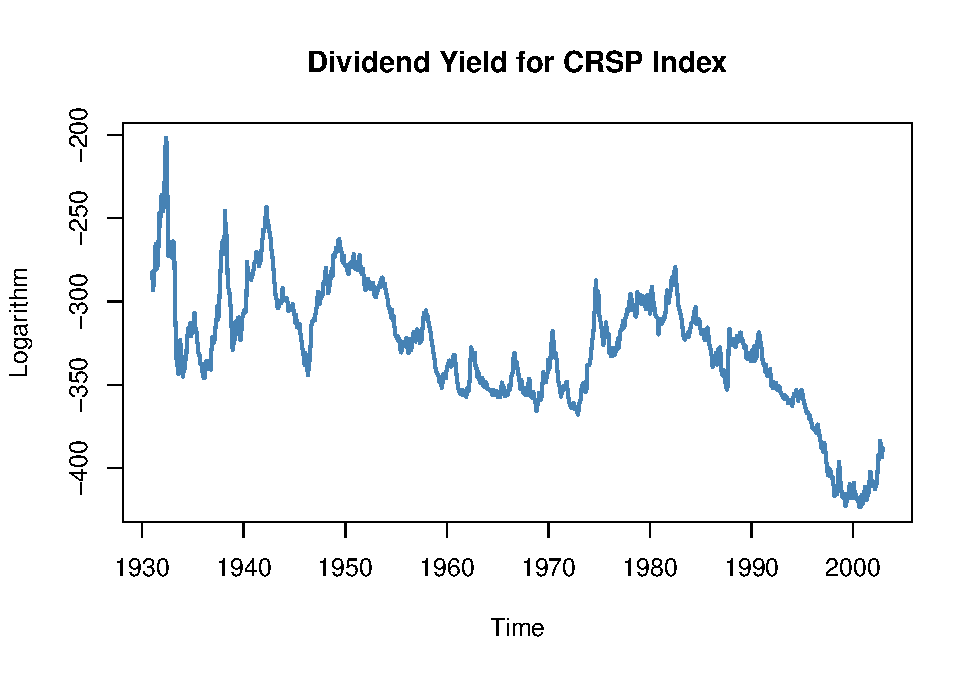
\includegraphics{URFITE_files/figure-latex/unnamed-chunk-67-1} \end{center}

The deviations from the standard normal distribution are significant:
both Dickey-Fuller distributions are skewed to the left and have a
havier left tail than the standard normal distribution.

\subsubsection*{Does U.S. GDP Have a Unit
Root?}\label{does-u.s.-gdp-have-a-unit-root}
\addcontentsline{toc}{subsubsection}{Does U.S. GDP Have a Unit Root?}

As an empirical example, we use the ADF test to assess whether there is
a stochastic trend in U.S. GDP using the regression

\begin{align*}
  \Delta\log(GDP_t) = \beta_0 + \alpha t + \beta_1 \log(GDP_{t-1}) + \beta_2 \Delta \log(GDP_{t-1}) + \beta_3 \Delta \log(GDP_{t-2}) + u_t.
\end{align*}

\begin{Shaded}
\begin{Highlighting}[]
\CommentTok{# generate log GDP series}
\NormalTok{LogGDP <-}\StringTok{ }\KeywordTok{ts}\NormalTok{(}\KeywordTok{log}\NormalTok{(GDP[}\StringTok{"1962::2012"}\NormalTok{]))}

\CommentTok{# estimate the model}
\KeywordTok{coeftest}\NormalTok{(}
  \KeywordTok{dynlm}\NormalTok{(}\KeywordTok{diff}\NormalTok{(LogGDP) }\OperatorTok{~}\StringTok{ }\KeywordTok{trend}\NormalTok{(LogGDP, }\DataTypeTok{scale =}\NormalTok{ F) }\OperatorTok{+}\StringTok{ }\KeywordTok{L}\NormalTok{(LogGDP) }\OperatorTok{+}\StringTok{ }\KeywordTok{diff}\NormalTok{(}\KeywordTok{L}\NormalTok{(LogGDP)) }\OperatorTok{+}\StringTok{ }\KeywordTok{diff}\NormalTok{(}\KeywordTok{L}\NormalTok{(LogGDP), }\DecValTok{2}\NormalTok{))}
\NormalTok{  )}
\end{Highlighting}
\end{Shaded}

\begin{verbatim}
## 
## t test of coefficients:
## 
##                             Estimate  Std. Error t value Pr(>|t|)   
## (Intercept)               0.27877045  0.11793233  2.3638 0.019066 * 
## trend(LogGDP, scale = F)  0.00023818  0.00011090  2.1476 0.032970 * 
## L(LogGDP)                -0.03332452  0.01441436 -2.3119 0.021822 * 
## diff(L(LogGDP))           0.08317976  0.11295542  0.7364 0.462371   
## diff(L(LogGDP), 2)        0.18763384  0.07055574  2.6594 0.008476 **
## ---
## Signif. codes:  0 '***' 0.001 '**' 0.01 '*' 0.05 '.' 0.1 ' ' 1
\end{verbatim}

The estimation yields

\begin{align*}
  \Delta\log(GDP_t) =& \, \underset{(0.118)}{0.28} + \underset{(0.0001)}{0.0002} t + -\underset{(0.014)}{0.033} \log(GDP_{t-1}) \\
  & \, + \underset{(0.113)}{0.083} \Delta \log(GDP_{t-1}) + \underset{(0.071)}{0.188} \Delta \log(GDP_{t-2}) + u_t,
\end{align*}

so the ADF test statistic is \(t=-0.033/0.014 = - 2.35\). The
corresponding \(5\%\) critical value from table \ref{tab:DFcrits} is
\(-3.41\) so we cannot reject the null hypothesis that \(\log(GDP)\) has
a stochastic trend in favour of the alternative that it is stationary
around a deterministic linear time trend.

\section{Nonstationarity II: Breaks}\label{nonstationarity-ii-breaks}

When there are discrete (at a distinct date) or gradual (over time)
changes in the population regression ceofficients, the series is
nonstationary. These changes are called \emph{breaks}. There is a
variety of reasons why breaks can occur in macroeconomic time series but
most often them are related to changes in economic policy or major
changes in the structure of the economy. See Chapter 14.7 for a
discussion of examples.

If breaks are not accounted for in the regression model, OLS estimates
will reflect the average relationship. Since these estimates might be
strongly misleading and result in poor forecast quality, we are
interested in testing for breaks. One distinguishes between testing for
a break when the date is known and testing for a break with an unknown
break date.

Let \(\tau\) denote a known break date and let \(D_t(\tau)\) be a binary
variable indicating time periods before and after the break.
Incorporating the break in an ADL(\(1\),\(1\)) regression model yields

\begin{align*}
  Y_t =& \beta_0 + \beta_1 Y_{t-1} + \delta_1 X_{t-1} + \gamma_0 D_t(\tau) + \left[ D_t(\tau) Y_{t-1}\right] \\ &+ \, \gamma_2\left[ D_t(\tau) X_{t-1} \right] + u_t,
\end{align*}

where we allow for discrete changes in \(\beta_0\), \(\beta_1\) and
\(\beta_2\) at the break date \(\tau\). The null hypothesis of no break,
\[H_0: \gamma_0=\gamma_1=\gamma_2=0,\] can be tested against the
alternative that at least one of the \(\gamma\)'s is not zero using an
\(F\)-Test. This idea is called a Chow test after Gregory Chow (1960).

When the break date is unknown the \emph{Quandt likelihood ratio} (QLR)
\emph{test} (Quandt, 1960) may be used. It is a modified version of the
Chow test which uses the largest of all \(F\)-statistics obtained when
applying the Chow test for all possible break dates in a predetermined
range \(\left[\tau_0,\tau_1\right]\). The QLR test is summarized in Key
Concept 14.9.

Key Concept 14.9

The QLR Test for Coefficient Stability

The QLR test can be used to test for a break in the population
regression function if the date of the break is unknown. The QLR test
statistic is the largest (Chow) \(F(\tau)\)-statistic computed over a
range of eligible break dates \(\tau_0 \leq \tau \leq \tau_1\):

\begin{align}
  QLR = \max\left[F(\tau_0),F(\tau_0 +1),\dots,F(\tau_1)\right]. \label{eq:QLRstatistic}
\end{align}

The most important properties are:

\begin{itemize}
\item
  The QLR test can be applied to test whether a subset of the
  coefficients in the population regression function breaks but the test
  also rejects if there is a slow evolution of the regression function.
\item
  When there is a single discrete break in the population regression
  function, the \(QLR\) test statistic is \(F(\widehat{\tau})\) and
  \(\widehat{\tau}/T\) is a consistent estimator of the true break date.
\item
  The large-sample distribution of \(QLR\) depends on \(q\), the number
  of restrictions beeing tested and both ratios of end points to the
  sample size, \(\tau_0/T, \tau_1/T\).
\item
  Similar to the ADF test, the large-sample distribution of \(QLR\) is
  nonstandard. Cricital values are presented in Table 14.5 of the book.
\end{itemize}

\subsubsection*{Has the Predictive Power of the term spread been
stable?}\label{has-the-predictive-power-of-the-term-spread-been-stable}
\addcontentsline{toc}{subsubsection}{Has the Predictive Power of the
term spread been stable?}

Using the QLR statistic we may test whether there is a break in the
coefficients on the lags of the term spread in \eqref{eq:gdpgradl22}, the
ADL(\(2\),\(2\)) regression model of GDP growth. Following Key Concept
14.9 we modify the specification of \eqref{eq:gdpgradl22} by adding a
break dummy \(D(\tau)\) and its interactions with both lags of term
spread and choose the range of break points to be tested as 1970:Q1 -
2005:Q2 (these periods are the center 70\% of the sample data from
1962:Q2 - 2012:Q4). Thus, the model becomes

\begin{align*}
    GDPGR_t =& \, \beta_0 + \beta_1 GDPGR_{t-1} + \beta_2 GDPGR_{t-2} \\
            &\,+  \beta_3  TSpread_{t-1} + \beta_4 TSpread_{t-2} \\
            &\,+ \gamma_1 D(\tau) + \gamma_2 (D(\tau) TSpread_{t-1}) \\
            &\,+ \gamma_3 (D(\tau) TSpread_{t-2}) \\
            &\,+ u_t.
\end{align*}

Next, we estimate the model for each break point and compute the
\(F\)-statistic corresponding to the null hypothesis
\(H_0: \gamma_1=\gamma_2=\gamma_3=0\). The \(QLR\)-statistic is the
largest of the \(F\)-statistics obtained in this manner.

\begin{Shaded}
\begin{Highlighting}[]
\CommentTok{# set up a range of possible break dates}
\NormalTok{tau <-}\StringTok{ }\KeywordTok{seq}\NormalTok{(}\DecValTok{1970}\NormalTok{, }\DecValTok{2005}\NormalTok{, }\FloatTok{0.25}\NormalTok{)}

\CommentTok{# initialize vector of F-statistics}
\NormalTok{Fstats <-}\StringTok{ }\KeywordTok{numeric}\NormalTok{(}\KeywordTok{length}\NormalTok{(tau))}

\CommentTok{# estimation loop over break dates}
\ControlFlowTok{for}\NormalTok{(i }\ControlFlowTok{in} \DecValTok{1}\OperatorTok{:}\KeywordTok{length}\NormalTok{(tau)) \{}

  \CommentTok{# set up dummy variable}
\NormalTok{  D <-}\StringTok{ }\KeywordTok{time}\NormalTok{(GDPGrowth_ts) }\OperatorTok{>}\StringTok{ }\NormalTok{tau[i]}

  \CommentTok{# estimate ADL(2,2) model with intercations}
\NormalTok{  test <-}\StringTok{ }\KeywordTok{dynlm}\NormalTok{(GDPGrowth_ts }\OperatorTok{~}\StringTok{ }\KeywordTok{L}\NormalTok{(GDPGrowth_ts) }\OperatorTok{+}\StringTok{ }\KeywordTok{L}\NormalTok{(GDPGrowth_ts, }\DecValTok{2}\NormalTok{) }\OperatorTok{+}\StringTok{ }
\StringTok{                  }\NormalTok{D}\OperatorTok{*}\KeywordTok{L}\NormalTok{(TSpread_ts) }\OperatorTok{+}\StringTok{ }\NormalTok{D}\OperatorTok{*}\KeywordTok{L}\NormalTok{(TSpread_ts, }\DecValTok{2}\NormalTok{),}
                \DataTypeTok{start =} \KeywordTok{c}\NormalTok{(}\DecValTok{1962}\NormalTok{, }\DecValTok{1}\NormalTok{), }
                \DataTypeTok{end =} \KeywordTok{c}\NormalTok{(}\DecValTok{2012}\NormalTok{, }\DecValTok{4}\NormalTok{))}
  
  \CommentTok{# compute and save the F-statistic}
\NormalTok{  Fstats[i] <-}\StringTok{ }\KeywordTok{linearHypothesis}\NormalTok{(test, }
                                \KeywordTok{c}\NormalTok{(}\StringTok{"DTRUE=0"}\NormalTok{, }\StringTok{"DTRUE:L(TSpread_ts)"}\NormalTok{, }\StringTok{"DTRUE:L(TSpread_ts, 2)"}\NormalTok{),}
                                \DataTypeTok{vcov. =}\NormalTok{ sandwich)}\OperatorTok{$}\NormalTok{F[}\DecValTok{2}\NormalTok{]}

\NormalTok{\}}
\end{Highlighting}
\end{Shaded}

We determine the \(QLR\) statistic using \texttt{max()}.

\begin{Shaded}
\begin{Highlighting}[]
\CommentTok{# identify QLR statistic}
\NormalTok{QLR <-}\StringTok{ }\KeywordTok{max}\NormalTok{(Fstats)}
\NormalTok{QLR}
\end{Highlighting}
\end{Shaded}

\begin{verbatim}
## [1] 6.651156
\end{verbatim}

It is straightforward to check that the \(QLR\)-statistic is the
\(F\)-statistic obtained for the regression where 1980:Q4 is chosen as
the break date.

\begin{Shaded}
\begin{Highlighting}[]
\CommentTok{# identify the time period where the QLR-statistic is observed}
\KeywordTok{as.yearqtr}\NormalTok{(}
\NormalTok{  tau[}\KeywordTok{which.max}\NormalTok{(Fstats)]}
\NormalTok{)}
\end{Highlighting}
\end{Shaded}

\begin{verbatim}
## [1] "1980 Q4"
\end{verbatim}

Since \(q=3\) hypotheses are tested and the central \(70\%\) of the
sample are considered to contain breaks, the corresponding \(1\%\)
critical value of the \(QLR\) test is \(6.02\). We reject the null
hypothesis that all coefficients (the coefficients on both lags of term
spread and the intercept) are stable since the computed
\(QLR\)-statistic exceeds this threshold. Thus evidence from the \(QLR\)
test suggests that there is a break in the ADL(\(2\),\(2\)) model of GDP
growth in the early 1980s.

To reproduce Figure 14.5 of the book, we convert the vector of
sequential break-point \(F\)-statistics into a time series object and
then generate a simple plot with some annotations.

\begin{Shaded}
\begin{Highlighting}[]
\CommentTok{# series of F-statistics}
\NormalTok{Fstatsseries <-}\StringTok{ }\KeywordTok{ts}\NormalTok{(Fstats, }
                   \DataTypeTok{start =}\NormalTok{ tau[}\DecValTok{1}\NormalTok{], }
                   \DataTypeTok{end =}\NormalTok{ tau[}\KeywordTok{length}\NormalTok{(tau)], }
                   \DataTypeTok{frequency =} \DecValTok{4}\NormalTok{)}

\CommentTok{# plot the F-statistics }
\KeywordTok{plot}\NormalTok{(Fstatsseries, }
     \DataTypeTok{xlim =} \KeywordTok{c}\NormalTok{(}\DecValTok{1960}\NormalTok{, }\DecValTok{2015}\NormalTok{),}
     \DataTypeTok{ylim =} \KeywordTok{c}\NormalTok{(}\DecValTok{1}\NormalTok{, }\FloatTok{7.5}\NormalTok{),}
     \DataTypeTok{lwd =} \DecValTok{2}\NormalTok{,}
     \DataTypeTok{col =} \StringTok{"steelblue"}\NormalTok{,}
     \DataTypeTok{ylab =} \StringTok{"F-Statistic"}\NormalTok{,}
     \DataTypeTok{xlab =} \StringTok{"Break Date"}\NormalTok{,}
     \DataTypeTok{main =} \StringTok{"Testing for a Break in GDP ADL(2,2) Regression at Different Dates"}
\NormalTok{     )}

\CommentTok{# dashed horizontal lines for critical values and QLR statistic}
\KeywordTok{abline}\NormalTok{(}\DataTypeTok{h =} \FloatTok{4.71}\NormalTok{, }\DataTypeTok{lty =} \DecValTok{2}\NormalTok{)}
\KeywordTok{abline}\NormalTok{(}\DataTypeTok{h =} \FloatTok{6.02}\NormalTok{, }\DataTypeTok{lty =} \DecValTok{2}\NormalTok{)}
\KeywordTok{segments}\NormalTok{(}\DecValTok{0}\NormalTok{, QLR, }\FloatTok{1980.75}\NormalTok{, QLR, }\DataTypeTok{col =} \StringTok{"darkred"}\NormalTok{)}
\KeywordTok{text}\NormalTok{(}\DecValTok{2010}\NormalTok{, }\FloatTok{6.2}\NormalTok{, }\StringTok{"1% Critical Value"}\NormalTok{)}
\KeywordTok{text}\NormalTok{(}\DecValTok{2010}\NormalTok{, }\FloatTok{4.9}\NormalTok{, }\StringTok{"5% Critical Value"}\NormalTok{)}
\KeywordTok{text}\NormalTok{(}\FloatTok{1980.75}\NormalTok{, QLR}\OperatorTok{+}\FloatTok{0.2}\NormalTok{, }\StringTok{"QLR Statistic"}\NormalTok{)}
\end{Highlighting}
\end{Shaded}

\begin{center}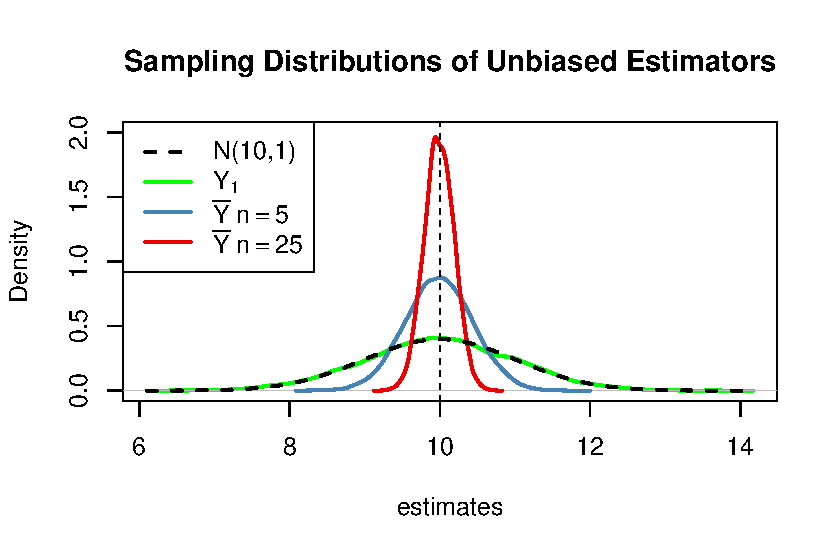
\includegraphics{URFITE_files/figure-latex/unnamed-chunk-72-1} \end{center}

\subsubsection*{Pseudo Out-of-Sample
Forecasting}\label{pseudo-out-of-sample-forecasting}
\addcontentsline{toc}{subsubsection}{Pseudo Out-of-Sample Forecasting}

Pseudo out-of-sample forecasts are used to simulate the out-of-sample
performance (the real time forecast performance) of a time series
regression model. In particular, pseudo out-of-sample forecast allow
estimation of the \(RMSFE\) of the model and enable researchers to
compare different model specifications with respect to their
reliability. Key Concept 14.10 summarizes this idea.

Key Concept 14.10

Pseudo Out-of-Sample Forecasting

\begin{enumerate}
\def\labelenumi{\arabic{enumi}.}
\item
  Divide the sample data into \(s=T-P\) and \(P\) subsequent
  overservations. The \(P\) observations are used as
  pseudo-out-of-sample observations.
\item
  Estimate the model using the first \(s\) observations.
\item
  Compute the pseudo-forecast \(\overset{\sim}{Y}_{s+1\vert s}\).
\item
  Compute the pseudo-forecast-error
  \(\overset{\sim}{u}_{s+1} = Y_{s+1} - \overset{\sim}{Y}_{s+1\vert s}\).
\item
  Repeat stepts 2 trough 4 for all reamaining pseudo-out-of-sample
  dates.
\end{enumerate}

\subsubsection*{Did the Predictive Power of the Term Spread Change
During the
2000s?}\label{did-the-predictive-power-of-the-term-spread-change-during-the-2000s}
\addcontentsline{toc}{subsubsection}{Did the Predictive Power of the
Term Spread Change During the 2000s?}

The insight gained in the previous section gives reason to presume that
the pseudo-out-of-sample performance of ADL(\(2\),\(2\)) models
estimated using data after the break in the early 1980s should not
deteriorate: provided that the coefficients of the population regression
function are stable after the potential break in 1980:Q4, these models
should have good predictive power. We check this by computing
pseudo-out-of-sample forecasts for the period 2003:Q1 - 2012:Q4, a range
covering 40 periods, where the forecast for 2003:Q1 is done using data
from 1981:Q1 - 2002:Q4, the forecast for 2003:Q2 is based on data frome
1981:Q1 - 2003:Q1 and so on.

Similarly as for the \(QLR\)-test we use a \texttt{for()} loop for
estimation of all 40 models and gather their \(SER\)s and the obtained
forecasts in a vector which is then used to compute pseudo-out-of-sample
forecast errors.

\begin{Shaded}
\begin{Highlighting}[]
\CommentTok{# end of sample dates}
\NormalTok{EndOfSample <-}\StringTok{ }\KeywordTok{seq}\NormalTok{(}\FloatTok{2002.75}\NormalTok{, }\FloatTok{2012.5}\NormalTok{, }\FloatTok{0.25}\NormalTok{)}

\NormalTok{forecasts <-}\StringTok{ }\KeywordTok{numeric}\NormalTok{(}\KeywordTok{length}\NormalTok{(EndOfSample))}
\NormalTok{SER <-}\StringTok{ }\NormalTok{forecasts}

\CommentTok{# estimation loop over end of sample dates}
\ControlFlowTok{for}\NormalTok{(i }\ControlFlowTok{in} \DecValTok{1}\OperatorTok{:}\KeywordTok{length}\NormalTok{(EndOfSample)) \{}

  \CommentTok{# estimate ADL(2,2) model}
\NormalTok{  m <-}\StringTok{ }\KeywordTok{dynlm}\NormalTok{(GDPGrowth_ts }\OperatorTok{~}\StringTok{ }\KeywordTok{L}\NormalTok{(GDPGrowth_ts) }\OperatorTok{+}\StringTok{ }\KeywordTok{L}\NormalTok{(GDPGrowth_ts, }\DecValTok{2}\NormalTok{) }\OperatorTok{+}\StringTok{ }\KeywordTok{L}\NormalTok{(TSpread_ts) }\OperatorTok{+}\StringTok{ }\KeywordTok{L}\NormalTok{(TSpread_ts, }\DecValTok{2}\NormalTok{), }
                \DataTypeTok{start =} \KeywordTok{c}\NormalTok{(}\DecValTok{1981}\NormalTok{, }\DecValTok{1}\NormalTok{), }
                \DataTypeTok{end =}\NormalTok{ EndOfSample[i])}
  
\NormalTok{  SER[i] <-}\StringTok{ }\KeywordTok{summary}\NormalTok{(m)}\OperatorTok{$}\NormalTok{sigma}
  
  \CommentTok{# sample data for one-period ahead forecast}
\NormalTok{  t <-}\StringTok{ }\KeywordTok{window}\NormalTok{(ADLdata, EndOfSample[i]}\OperatorTok{-}\FloatTok{0.25}\NormalTok{, EndOfSample[i])}
  
  \CommentTok{# compute forecast}
\NormalTok{  forecasts[i] <-}\StringTok{ }\KeywordTok{coef}\NormalTok{(m) }\OperatorTok\StringTok{ }\KeywordTok{c}\NormalTok{(}\DecValTok{1}\NormalTok{, t[}\DecValTok{1}\NormalTok{, }\DecValTok{1}\NormalTok{], t[}\DecValTok{2}\NormalTok{, }\DecValTok{1}\NormalTok{], t[}\DecValTok{1}\NormalTok{, }\DecValTok{2}\NormalTok{], t[}\DecValTok{2}\NormalTok{, }\DecValTok{2}\NormalTok{]) }
\NormalTok{\}}
\end{Highlighting}
\end{Shaded}

\begin{Shaded}
\begin{Highlighting}[]
\CommentTok{# compute psuedo-out-of-sample forecast errors}
\NormalTok{POOSFCE <-}\StringTok{ }\KeywordTok{window}\NormalTok{(GDPGrowth_ts, }\KeywordTok{c}\NormalTok{(}\DecValTok{2003}\NormalTok{, }\DecValTok{1}\NormalTok{), }\KeywordTok{c}\NormalTok{(}\DecValTok{2012}\NormalTok{, }\DecValTok{4}\NormalTok{)) }\OperatorTok{-}\StringTok{ }\NormalTok{forecasts}
\end{Highlighting}
\end{Shaded}

We next translate the pseudo-out-of-sample forecasts into an object of
class ts and plot the real GDP growth rate against the forecasted
series.

\begin{Shaded}
\begin{Highlighting}[]
\CommentTok{# series of pseudo-out-of-sample forecasts}
\NormalTok{PSOSSFc <-}\StringTok{ }\KeywordTok{ts}\NormalTok{(forecasts, }
              \DataTypeTok{start =} \DecValTok{2003}\NormalTok{, }
              \DataTypeTok{end =} \FloatTok{2012.75}\NormalTok{, }
              \DataTypeTok{frequency =} \DecValTok{4}\NormalTok{)}

\CommentTok{# plot GDP growth time series}
\KeywordTok{plot}\NormalTok{(}\KeywordTok{window}\NormalTok{(GDPGrowth_ts, }\KeywordTok{c}\NormalTok{(}\DecValTok{2003}\NormalTok{, }\DecValTok{1}\NormalTok{), }\KeywordTok{c}\NormalTok{(}\DecValTok{2012}\NormalTok{, }\DecValTok{4}\NormalTok{)),}
     \DataTypeTok{col =} \StringTok{"steelblue"}\NormalTok{,}
     \DataTypeTok{lwd =} \DecValTok{2}\NormalTok{,}
     \DataTypeTok{ylab =} \StringTok{"Percent"}\NormalTok{,}
     \DataTypeTok{main =} \StringTok{"Pseudo-Out-Of-Sample Forecasts of GDP Growth"}
\NormalTok{     )}

\CommentTok{# add series of pseudo-out-of-sample forecasts}
\KeywordTok{lines}\NormalTok{(PSOSSFc, }
      \DataTypeTok{lwd =} \DecValTok{2}\NormalTok{, }
      \DataTypeTok{lty =} \DecValTok{2}
\NormalTok{      )}

\CommentTok{# shade area between curves (the pseudo forecast error)}
\KeywordTok{polygon}\NormalTok{(}\KeywordTok{c}\NormalTok{(}\KeywordTok{time}\NormalTok{(PSOSSFc), }\KeywordTok{rev}\NormalTok{(}\KeywordTok{time}\NormalTok{(PSOSSFc))), }
        \KeywordTok{c}\NormalTok{(}\KeywordTok{window}\NormalTok{(GDPGrowth_ts, }\KeywordTok{c}\NormalTok{(}\DecValTok{2003}\NormalTok{, }\DecValTok{1}\NormalTok{), }\KeywordTok{c}\NormalTok{(}\DecValTok{2012}\NormalTok{, }\DecValTok{4}\NormalTok{)), }\KeywordTok{rev}\NormalTok{(PSOSSFc)),}
        \DataTypeTok{col =} \KeywordTok{alpha}\NormalTok{(}\StringTok{"blue"}\NormalTok{, }\DataTypeTok{alpha =} \FloatTok{0.3}\NormalTok{),}
        \DataTypeTok{border =} \OtherTok{NA}
\NormalTok{        )}

\CommentTok{# add a legend}
\KeywordTok{legend}\NormalTok{(}\StringTok{"bottomleft"}\NormalTok{, }
       \DataTypeTok{lty =} \KeywordTok{c}\NormalTok{(}\DecValTok{1}\NormalTok{, }\DecValTok{2}\NormalTok{, }\DecValTok{1}\NormalTok{),}
       \DataTypeTok{lwd =} \KeywordTok{c}\NormalTok{(}\DecValTok{2}\NormalTok{, }\DecValTok{2}\NormalTok{, }\DecValTok{10}\NormalTok{),}
       \DataTypeTok{col =} \KeywordTok{c}\NormalTok{(}\StringTok{"steelblue"}\NormalTok{,}\StringTok{"black"}\NormalTok{,}\KeywordTok{alpha}\NormalTok{(}\StringTok{"blue"}\NormalTok{, }\DataTypeTok{alpha =} \FloatTok{0.3}\NormalTok{)), }
       \DataTypeTok{legend =} \KeywordTok{c}\NormalTok{(}\StringTok{"Actual GDP growth rate"}\NormalTok{,}
         \StringTok{"Forecasted GDP growth rate"}\NormalTok{,}
         \StringTok{"Pseudo forecast Error"}\NormalTok{)}
\NormalTok{       )}
\end{Highlighting}
\end{Shaded}

\begin{center}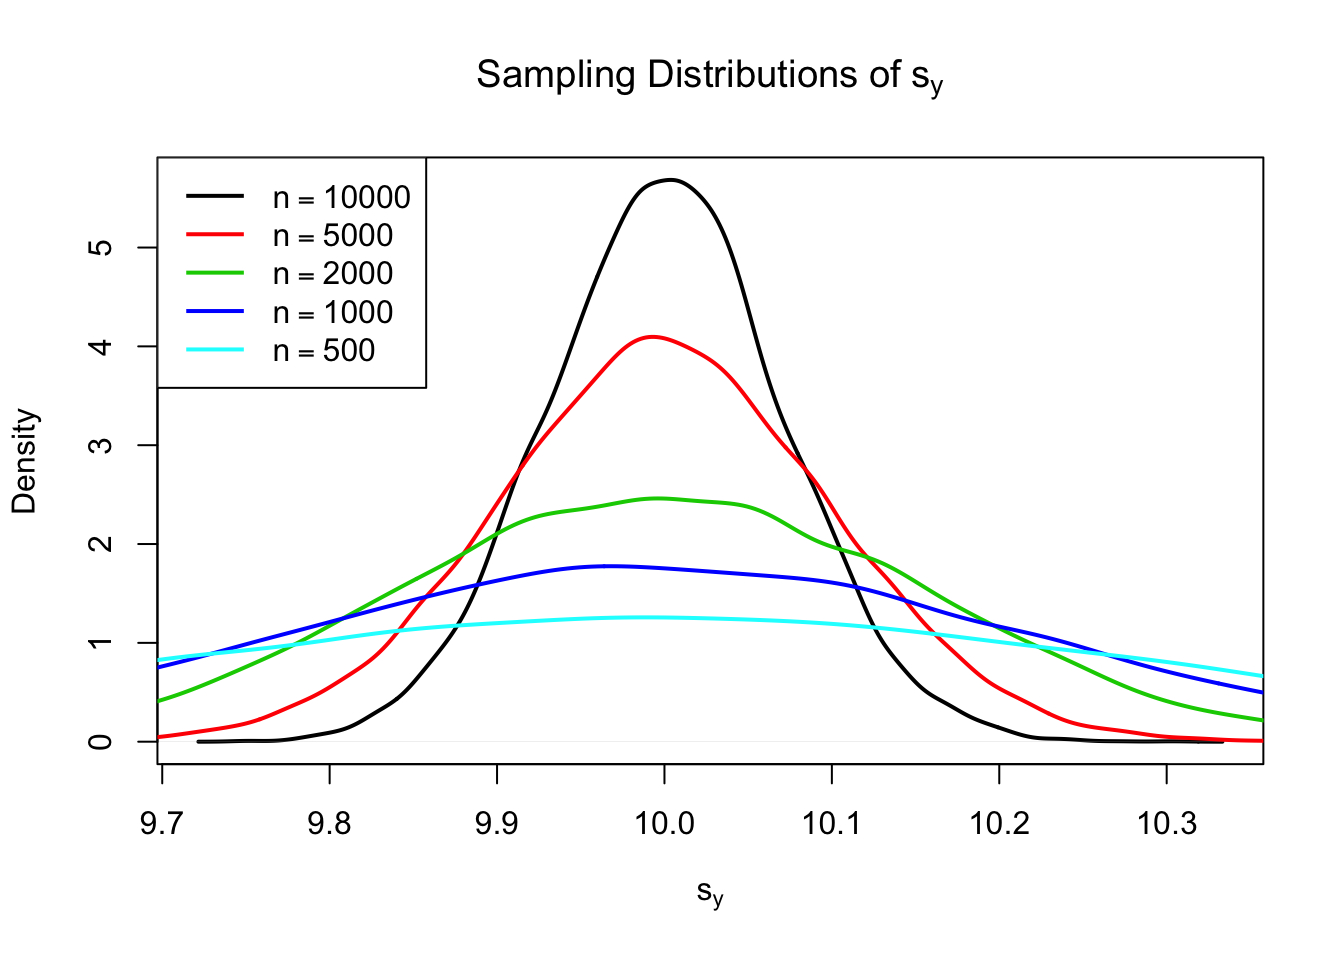
\includegraphics{URFITE_files/figure-latex/unnamed-chunk-75-1} \end{center}

Apparently, the pseudo forecasts track the actual GDP growth rate quite
well, except for the kink in 2009 which can be attributed to the recent
financial crisis.

The \(SER\) of the first model (estimated using data from 1981:Q1 to
2002:Q4) is \(2.39\) so based on the in-sample fit we would expect the
out of sample forecast errors to have mean zero and a mean squared
forecast error of about \(2.39\).

\begin{Shaded}
\begin{Highlighting}[]
\CommentTok{# SER of ADL(2,2) mode using data from 1981:Q1 - 2002:Q4}
\NormalTok{SER[}\DecValTok{1}\NormalTok{]}
\end{Highlighting}
\end{Shaded}

\begin{verbatim}
## [1] 2.389773
\end{verbatim}

The root mean squared forecast error of the pseudo-out-of-sample
forecasts is somewhat larger.

\begin{Shaded}
\begin{Highlighting}[]
\CommentTok{# compute root mean squared forecast error}
\KeywordTok{sd}\NormalTok{(POOSFCE)}
\end{Highlighting}
\end{Shaded}

\begin{verbatim}
## [1] 2.667612
\end{verbatim}

An interesting hypothesis is whether the mean forecast error is zero,
that is the ADL(\(2\),\(2\)) forecasts are right, on average. This
hypothesis is easily tested using the function \texttt{t.test()}.

\begin{Shaded}
\begin{Highlighting}[]
\CommentTok{# test if mean forecast error is zero}
\KeywordTok{t.test}\NormalTok{(POOSFCE)}
\end{Highlighting}
\end{Shaded}

\begin{verbatim}
## 
##  One Sample t-test
## 
## data:  POOSFCE
## t = -1.5523, df = 39, p-value = 0.1287
## alternative hypothesis: true mean is not equal to 0
## 95 percent confidence interval:
##  -1.5078876  0.1984001
## sample estimates:
##  mean of x 
## -0.6547438
\end{verbatim}

The hypothesis cannot be rejected at the \(10\%\) significance level.
Alltogther the analysis suggests that the ADL(\(2\),\(2\)) model
coefficients have been stable since the presumed break in the early
1980s.

\section{Can You Beat the Market? Part
II}\label{can-you-beat-the-market-part-ii}

The dividend yield (the ratio of current dividens to the stock price)
can be considered as an indicator of future dividends: if a stock has a
high current dividend yield, it can be considered undervalued and it can
be presumed that the price of the stock goes up in the future, meaning
that future excess returns go up.

This presumption can be examined using ADL models of exess returns,
where lags of the logarithm of the stock's dividend yield serve as
additional regressors.

Unfortunatly, a graphical inspection of the time series of the logarithm
of the dividend yield casts doubt on the assumption that the series is
stationary which, as has been discussed in Chapter 14.7, is necessary to
obtain meaningful results in a regression analysis.

\begin{Shaded}
\begin{Highlighting}[]
\CommentTok{# plot logarithm of dividend yield series}
\KeywordTok{plot}\NormalTok{(StockReturns[, }\DecValTok{2}\NormalTok{], }
     \DataTypeTok{col =} \StringTok{"steelblue"}\NormalTok{, }
     \DataTypeTok{lwd =} \DecValTok{2}\NormalTok{, }
     \DataTypeTok{ylab =} \StringTok{"Logarithm"}\NormalTok{, }
     \DataTypeTok{main =} \StringTok{"Dividend Yield for CRSP Index"}\NormalTok{)}
\end{Highlighting}
\end{Shaded}

\begin{center}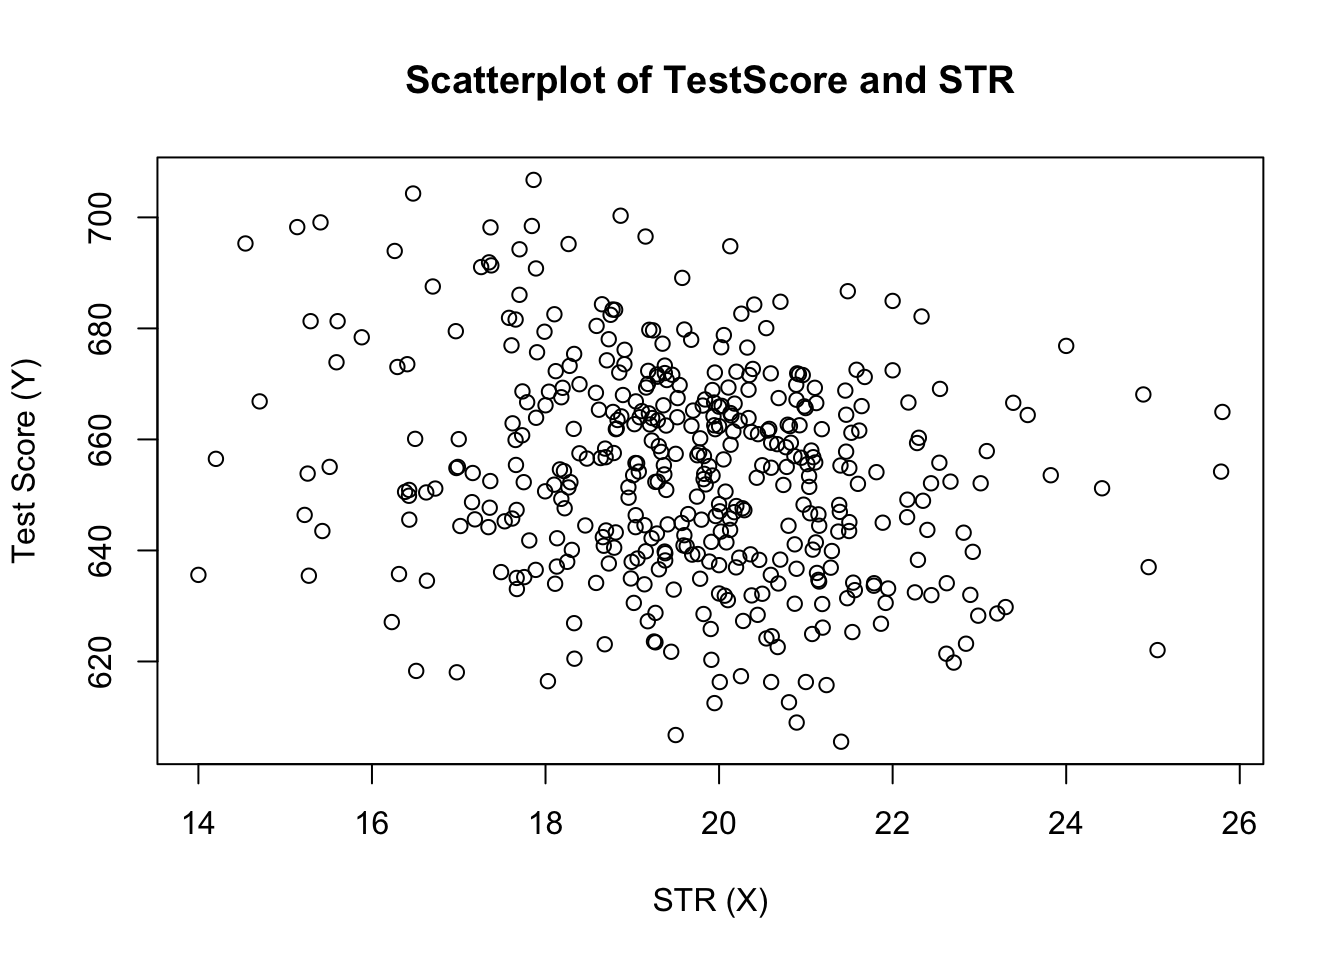
\includegraphics{URFITE_files/figure-latex/unnamed-chunk-79-1} \end{center}

The Dickey-Fuller test statistic for an autoregressive unit root in an
AR(\(1\)) model with drift provides further evidence that the series
might be nonstationary.

\begin{Shaded}
\begin{Highlighting}[]
\CommentTok{# DF-Regression for log dividend yield}
\NormalTok{LDivYield <-}\StringTok{ }\KeywordTok{dynlm}\NormalTok{(}\KeywordTok{d}\NormalTok{(ln_DivYield) }\OperatorTok{~}\StringTok{ }\KeywordTok{L}\NormalTok{(ln_DivYield), }\DataTypeTok{data =}\NormalTok{ StockReturns,}
      \DataTypeTok{start =} \KeywordTok{c}\NormalTok{(}\DecValTok{1960}\NormalTok{, }\DecValTok{1}\NormalTok{), }\DataTypeTok{end =} \KeywordTok{c}\NormalTok{(}\DecValTok{2002}\NormalTok{, }\DecValTok{12}\NormalTok{)}
\NormalTok{      )}

\KeywordTok{summary}\NormalTok{(LDivYield)}\OperatorTok{$}\NormalTok{coef}
\end{Highlighting}
\end{Shaded}

\begin{verbatim}
##                    Estimate  Std. Error   t value  Pr(>|t|)
## (Intercept)    -2.728786496 2.083152348 -1.309931 0.1908042
## L(ln_DivYield) -0.007656929 0.005998017 -1.276577 0.2023282
\end{verbatim}

Since the \(t\)-value for the coefficient on the lagged logarithm of the
dividend yield is \(-1.27\), the hypothesis that the true coefficient is
zero cannot be rejected, even at the \(10\%\) significance level.

However, it is possible to examine whether the dividend yield has
predictive power for excess returns by using its differences in an
ADL(\(1\),\(1\)) and an ADL(\(2\),\(2\)) model (remember that
differencing a series with a unit root yields a stationary series)
although these model specifications do not correspond to the ecnonomic
reasoning mentioned above. Thus we also estimate a ADL(\(1\),\(1\))
regression using the level of the logarithm of the dividend yield.

Altogether we estimate three different model specifications:

\begin{align*}
  excess \, returns_t =& \, \beta_0 + \beta_1 excess \, returns_{t-1} + \beta_3 \Delta \log(dividend yield_{t-1}) + u_t \\
  \\
  excess \, returns_t =& \, \beta_0 + \beta_1 excess \, returns_{t-1} + \beta_2 excess \, returns_{t-2} \\ +& \, \beta_3 \Delta \log(dividend yield_{t-1}) + \beta_4 \Delta \log(dividend yield_{t-2}) + u_t \\
  \\
  excess \, returns_t =& \, \beta_0 + \beta_1 excess \, returns_{t-1} + \beta_5 \log(dividend yield_{t-1}) + u_t \\
\end{align*}

\begin{Shaded}
\begin{Highlighting}[]
\CommentTok{# ADL(1,1) (1st difference of log dividend yield)}
\NormalTok{CRSP_ADL_}\DecValTok{1}\NormalTok{ <-}\StringTok{ }\KeywordTok{dynlm}\NormalTok{(ExReturn }\OperatorTok{~}\StringTok{ }\KeywordTok{L}\NormalTok{(ExReturn) }\OperatorTok{+}\StringTok{ }\KeywordTok{d}\NormalTok{(}\KeywordTok{L}\NormalTok{(ln_DivYield)), }
                    \DataTypeTok{data =}\NormalTok{ StockReturns,}
                    \DataTypeTok{start =} \KeywordTok{c}\NormalTok{(}\DecValTok{1960}\NormalTok{, }\DecValTok{1}\NormalTok{), }\DataTypeTok{end =} \KeywordTok{c}\NormalTok{(}\DecValTok{2002}\NormalTok{, }\DecValTok{12}\NormalTok{)}
\NormalTok{              )}

\CommentTok{# ADL(2,2) (1st & 2nd differences of log dividend yield)}
\NormalTok{CRSP_ADL_}\DecValTok{2}\NormalTok{ <-}\StringTok{ }\KeywordTok{dynlm}\NormalTok{(ExReturn }\OperatorTok{~}\StringTok{ }\KeywordTok{L}\NormalTok{(ExReturn) }\OperatorTok{+}\StringTok{ }\KeywordTok{L}\NormalTok{(ExReturn, }\DecValTok{2}\NormalTok{) }\OperatorTok{+}\StringTok{ }\KeywordTok{d}\NormalTok{(}\KeywordTok{L}\NormalTok{(ln_DivYield)) }\OperatorTok{+}\StringTok{ }\KeywordTok{d}\NormalTok{(}\KeywordTok{L}\NormalTok{(ln_DivYield, }\DecValTok{2}\NormalTok{)), }
                   \DataTypeTok{data =}\NormalTok{ StockReturns,}
                   \DataTypeTok{start =} \KeywordTok{c}\NormalTok{(}\DecValTok{1960}\NormalTok{, }\DecValTok{1}\NormalTok{), }\DataTypeTok{end =} \KeywordTok{c}\NormalTok{(}\DecValTok{2002}\NormalTok{, }\DecValTok{12}\NormalTok{)}
\NormalTok{              )}

\CommentTok{# ADL(1,1) (level of log dividend yield)}
\NormalTok{CRSP_ADL_}\DecValTok{3}\NormalTok{ <-}\StringTok{ }\KeywordTok{dynlm}\NormalTok{(ExReturn }\OperatorTok{~}\StringTok{ }\KeywordTok{L}\NormalTok{(ExReturn) }\OperatorTok{+}\StringTok{ }\KeywordTok{L}\NormalTok{(ln_DivYield),}
                    \DataTypeTok{data =}\NormalTok{ StockReturns,}
                    \DataTypeTok{start =} \KeywordTok{c}\NormalTok{(}\DecValTok{1960}\NormalTok{, }\DecValTok{1}\NormalTok{), }\DataTypeTok{end =} \KeywordTok{c}\NormalTok{(}\DecValTok{1992}\NormalTok{, }\DecValTok{12}\NormalTok{)}
\NormalTok{              )}
\end{Highlighting}
\end{Shaded}

\begin{Shaded}
\begin{Highlighting}[]
\NormalTok{rob_se_CRSP_ADL <-}\StringTok{ }\KeywordTok{list}\NormalTok{(}
  \KeywordTok{sqrt}\NormalTok{(}\KeywordTok{diag}\NormalTok{(}\KeywordTok{sandwich}\NormalTok{(CRSP_ADL_}\DecValTok{1}\NormalTok{))),}
  \KeywordTok{sqrt}\NormalTok{(}\KeywordTok{diag}\NormalTok{(}\KeywordTok{sandwich}\NormalTok{(CRSP_ADL_}\DecValTok{2}\NormalTok{))),}
  \KeywordTok{sqrt}\NormalTok{(}\KeywordTok{diag}\NormalTok{(}\KeywordTok{sandwich}\NormalTok{(CRSP_ADL_}\DecValTok{3}\NormalTok{)))}
\NormalTok{)}
\end{Highlighting}
\end{Shaded}

A tabular representation of the results can then be generated using
\texttt{stargazer()}.

\begin{sidewaystable}[!htbp] \centering 
  \caption{ADL Models of Monthly Excess Stock Returns} 
  \label{} 
\begin{tabular}{@{\extracolsep{-5pt}}lccc} 
\\[-1.8ex]\hline 
\hline \\[-1.8ex] 
 & \multicolumn{3}{c}{Excess returns on the CSRP value-weighted index} \\ 
\cline{2-4} 
 & ADL(1,1) & ADL(2,2) & ADL(1,1) \\ 
\\[-1.8ex] & (1) & (2) & (3)\\ 
\hline \\[-1.8ex] 
 $excess return_{t-1}$ & 0.059 & 0.042 & 0.078 \\ 
  & (0.158) & (0.162) & (0.057) \\ 
  $excess return_{t-2}$ &  & $-$0.213 &  \\ 
  &  & (0.193) &  \\ 
  $1^{st} diff log(dividend yield_{t-1})$ & 0.009 & $-$0.012 &  \\ 
  & (0.157) & (0.163) &  \\ 
  $1^{st} diff log(dividend yield_{t-2})$ &  & $-$0.161 &  \\ 
  &  & (0.185) &  \\ 
  $log(dividend yield_{t-1})$ &  &  & 0.026$^{**}$ \\ 
  &  &  & (0.012) \\ 
  Constant & 0.309 & 0.372$^{*}$ & 8.987$^{**}$ \\ 
  & (0.199) & (0.208) & (3.912) \\ 
 \hline \\[-1.8ex] 
Observations & 516 & 516 & 396 \\ 
R$^{2}$ & 0.003 & 0.007 & 0.018 \\ 
Adjusted R$^{2}$ & $-$0.001 & $-$0.001 & 0.013 \\ 
Residual Std. Error & 4.338 (df = 513) & 4.337 (df = 511) & 4.407 (df = 393) \\ 
F Statistic & 0.653 (df = 2; 513) & 0.897 (df = 4; 511) & 3.683$^{**}$ (df = 2; 393) \\ 
\hline 
\hline \\[-1.8ex] 
\textit{Note:}  & \multicolumn{3}{r}{$^{*}$p$<$0.1; $^{**}$p$<$0.05; $^{***}$p$<$0.01} \\ 
\end{tabular} 
\end{sidewaystable}

Notice that for models (1) and (2) none of the individual
\(t\)-statistics suggest that the coefficients are different from zero.
Also we cannot reject the hypothesis that none of the lags have
predictive power for excess returns at any common level of significance
(an \(F\)-test that the lags have predictive power rejects for both
models).

Things are different for model (3). The coefficient on the level of the
logarithm of the devidend yield is different from zero at the \(5\%\)
level and the \(F\)-test does not reject at this level either. But we
should be suspicious: the high degree of persistence in the devidend
yield series probably renders this inference useless because \(t\)- and
\(F\)-statistics may follow distributions that deviate considerably from
their theoretical large-sample distributions such that the usual
critical values cannot be applied.

If model (3) would be of any use for predicting excess returns,
pseudo-out-of-sample forecasts based on (3) should outperform forecasts
of an intercept-only model in terms of the sample RMSFE. We can perform
this type of comparison using R code in the fashion of the applications
of Chapter 14.8.

\begin{Shaded}
\begin{Highlighting}[]
\CommentTok{# end of sample dates}
\NormalTok{EndOfSample <-}\StringTok{ }\KeywordTok{as.numeric}\NormalTok{(}\KeywordTok{window}\NormalTok{(}\KeywordTok{time}\NormalTok{(StockReturns), }\KeywordTok{c}\NormalTok{(}\DecValTok{1992}\NormalTok{, }\DecValTok{12}\NormalTok{), }\KeywordTok{c}\NormalTok{(}\DecValTok{2002}\NormalTok{, }\DecValTok{11}\NormalTok{)))}

\CommentTok{# initialize matrix  forecasts}
\NormalTok{forecasts <-}\StringTok{ }\KeywordTok{matrix}\NormalTok{(}\DataTypeTok{nrow =} \DecValTok{2}\NormalTok{, }
                    \DataTypeTok{ncol =} \KeywordTok{length}\NormalTok{(EndOfSample))}

\CommentTok{# estimation loop over end of sample dates}
\ControlFlowTok{for}\NormalTok{(i }\ControlFlowTok{in} \DecValTok{1}\OperatorTok{:}\KeywordTok{length}\NormalTok{(EndOfSample)) \{}

  \CommentTok{# estimate model (3)}
\NormalTok{  mod3 <-}\StringTok{ }\KeywordTok{dynlm}\NormalTok{(ExReturn }\OperatorTok{~}\StringTok{ }\KeywordTok{L}\NormalTok{(ExReturn) }\OperatorTok{+}\StringTok{ }\KeywordTok{L}\NormalTok{(ln_DivYield), }\DataTypeTok{data =}\NormalTok{ StockReturns, }
                \DataTypeTok{start =} \KeywordTok{c}\NormalTok{(}\DecValTok{1960}\NormalTok{, }\DecValTok{1}\NormalTok{), }
                \DataTypeTok{end =}\NormalTok{ EndOfSample[i])}
  
  \CommentTok{# estimate intercept only model}
\NormalTok{  modconst <-}\StringTok{ }\KeywordTok{dynlm}\NormalTok{(ExReturn }\OperatorTok{~}\StringTok{ }\DecValTok{1}\NormalTok{, }\DataTypeTok{data =}\NormalTok{ StockReturns, }
                \DataTypeTok{start =} \KeywordTok{c}\NormalTok{(}\DecValTok{1960}\NormalTok{, }\DecValTok{1}\NormalTok{), }
                \DataTypeTok{end =}\NormalTok{ EndOfSample[i])}
  
  \CommentTok{# sample data for one-period ahead forecast}
\NormalTok{  t <-}\StringTok{ }\KeywordTok{window}\NormalTok{(StockReturns, EndOfSample[i], EndOfSample[i])}
  
  \CommentTok{# compute forecast}
\NormalTok{  forecasts[,i] <-}\StringTok{ }\KeywordTok{c}\NormalTok{(}
    \KeywordTok{coef}\NormalTok{(mod3) }\OperatorTok\StringTok{ }\KeywordTok{c}\NormalTok{(}\DecValTok{1}\NormalTok{, t[}\DecValTok{1}\NormalTok{], t[}\DecValTok{2}\NormalTok{]),}
    \KeywordTok{coef}\NormalTok{(modconst)}
\NormalTok{  )}
                     
\NormalTok{\}}
\end{Highlighting}
\end{Shaded}

\begin{Shaded}
\begin{Highlighting}[]
\CommentTok{# gather data}
\NormalTok{d <-}\StringTok{ }\KeywordTok{cbind}\NormalTok{(}
  \StringTok{"Excess Returns"}\NormalTok{ =}\StringTok{ }\KeywordTok{c}\NormalTok{(}\KeywordTok{window}\NormalTok{(StockReturns[,}\DecValTok{1}\NormalTok{], }\KeywordTok{c}\NormalTok{(}\DecValTok{1993}\NormalTok{, }\DecValTok{1}\NormalTok{), }\KeywordTok{c}\NormalTok{(}\DecValTok{2002}\NormalTok{, }\DecValTok{12}\NormalTok{))),}
  \StringTok{"Model (3)"}\NormalTok{ =}\StringTok{ }\NormalTok{forecasts[}\DecValTok{1}\NormalTok{,], }
  \StringTok{"Intercept Only"}\NormalTok{ =}\StringTok{ }\NormalTok{forecasts[}\DecValTok{2}\NormalTok{,], }
  \StringTok{"Always Zero"}\NormalTok{ =}\StringTok{  }\DecValTok{0}\NormalTok{)}

\CommentTok{# Compute RMSFEs}
\KeywordTok{c}\NormalTok{(}
  \StringTok{"ADL model (3)"}\NormalTok{ =}\StringTok{ }\KeywordTok{sd}\NormalTok{(d[, }\DecValTok{1}\NormalTok{] }\OperatorTok{-}\StringTok{ }\NormalTok{d[, }\DecValTok{2}\NormalTok{]),}
  \StringTok{"Intercept-only model"}\NormalTok{ =}\StringTok{ }\KeywordTok{sd}\NormalTok{(d[, }\DecValTok{1}\NormalTok{] }\OperatorTok{-}\StringTok{ }\NormalTok{d[, }\DecValTok{3}\NormalTok{]),}
  \StringTok{"Always zero"}\NormalTok{ =}\StringTok{ }\KeywordTok{sd}\NormalTok{(d[,}\DecValTok{1}\NormalTok{] }\OperatorTok{-}\StringTok{ }\NormalTok{d[, }\DecValTok{4}\NormalTok{])}
\NormalTok{)}
\end{Highlighting}
\end{Shaded}

\begin{verbatim}
##        ADL model (3) Intercept-only model          Always zero 
##             4.043757             4.000221             3.995428
\end{verbatim}

The comparison indicates that model (3) is not useful since it is
outperformed in terms of sample RMSFE by the intercept-only model. A
model forecasting excess returns always to be zero has an even lower
sample RMSFE. This finding is consistent with the strong-form efficiency
hypothesis which states that all publicly available information is
accounted for in stock prices such that there is no way to predict
future stock prices or excess returns using past observations, implying
that the perceived significant relationship indicated by model (3) is
wrong.

\subsubsection*{Summary}\label{summary}
\addcontentsline{toc}{subsubsection}{Summary}

This chapter dealt with introductory topics in time series regression
analysis, where variables are generally correlated from one observation
to the next, a concept termed serial correlation. At the beginning,
several ways of storing and plotting time series data using R have been
presented and used for informal analysis of economic example data.

We have introduced AR and ADL models and applied them in the context of
forecasting of macroeconomic and financial time series using R. The
discussion also included the topic of lag length selection. It was shown
how to set up a simple function that computes the BIC for a model object
supplied.

We have also seen how to write simple R code for performing and
evaluating forecasts and demonstrated some more sophisticated approaches
to conduct pseudo-out-of-sample forecasts for assessment of a model's
predictive power for unobserved future outcomes of a series, to check
model stability and to compare different models.

Furthermore, some more technical aspects like the concept of
stationarity were adressed. This included applications to testing for an
autoregressive unit root with the Dickey-Fuller test and the detection
of a break in the population regression function using the \(QLR\)
statistic. For both methods, the distribution of the relevant test
statistic is nonnormal, even in large samples. Concerning the
Dickey-Fuller test we have used R's random number generation facilities
to produce evidence for this by means of a Monte-Carlo simulation and
motivated usage of the quantiles tabulated in the book.

Also, empirical studies regarding the validity of the weak and the
strong form efficiency hypothesis which are presented in the
applications \emph{Can You Beat the Market? Part I \& II} in the book
have been reproduced using R.

In all applications presented in this chapter, the focus was layed on
forecasting future outcomes rather than estimation of causal
relationships between time series variables. However, the framework of
methods needed for the latter is very similar. Chapter 15 is devoted to
estimation of so called \emph{dynamic causal effects}.

\bibliography{book.bib,packages.bib}


\end{document}
